%!TEX root = ../../thesis.tex

\chapter{Other backgrounds}
\label{chap:backgrounds}
%!TEX root = ../../thesis.tex

In addition to the \WW background, many other background processes contribute significantly. 
As they are often difficult to accurately model in the \HWW phase space, they are estimated by 
sophisticated data-driven methods. Even so, there is usually some underlying dependence upon 
MC (see \Table~\ref{tab:bkg:mc_samples}).

\begin{table}[b]
	\begin{tabular}{c@{\hskip 0.3in}c}
		\toprule
		Process & MC generator (\twojet bin) \\
		\midrule
		\WW        & \meps{\powhegbox}{\pythia{6}}, \meps{\ggtoww}{\fherwig} (\sherpa) \\
		\ttbar     & \meps{\powhegbox}{\pythia{6}} \\
		single top & \meps{\powhegbox}{\pythia{6}}, \meps{\acermc}{\pythia{6}} \\
		\Wjets     & \meps{\alpgen}{\fherwig} \\
		\DY        & \meps{\alpgen}{\fherwig} (\sherpa) \\
		\Wgamma    & \meps{\alpgen}{\fherwig} \\
		\WZ        & \meps{\powhegbox}{\pythia{8}} (\sherpa) \\
		\ZZ        & \meps{\powhegbox}{\pythia{8}}, \meps{\ggtozz}{\fherwig} (\sherpa) \\
		\Wgstar, \Zgstar, \Zgamma & \sherpa \\
		\bottomrule
	\end{tabular}
	\caption{MC generators used to model backgrounds to the \HWW search. These are used with 
	data-driven techniques described in the text.}
	\label{tab:bkg:mc_samples}
\end{table}

This chapter describes the estimation of non-\WW backgrounds: \Wjets and dijet in 
\Section~\ref{sec:wjets}, non-\WW diboson in \Section~\ref{sec:diboson}, top in 
\Section~\ref{sec:top}, and \DY in \Section~\ref{sec:dy}.

\section{\Wjets and dijet}
	\label{sec:wjets}
	%!TEX root = ../../thesis.tex

\Wjets events contribute to the background when a jet is misidentified as a lepton, and 
dijet events contribute when two jets are misidentified as leptons. This is due to leptonic 
decays of heavy flavour hadrons, hadronic showers mimicking the electromagnetic showers, or 
punchthrough into the muon spectrometer. Although the fake rates are very low, these 
backgrounds are significant because the \Wjets and dijet cross sections are many orders of 
magnitude larger than those of Higgs boson production. These fake rates are sensitive to 
effects that are difficult to accurately model (such as jet flavour composition, jet 
substructure and hadronic shower shapes), a data-driven \textit{fake factor method} is used 
to estimate these backgrounds.

As these two backgrounds have large uncertainties, their suppression is critically 
important. The electron and muon selection criteria are chosen to be tighter at low \pt 
(see \Section~\ref{sec:objects}), in order to reduce the fake rates where these backgrounds 
are largest. The dijet background is additionally rejected by requiring significant \met 
and by the \unit{$\maxmtw > 50$}{\GeV} cut in the 1-jet bin of the \emch/\mech channels.



\subsection{The fake factor method}
\label{sec:wjets:fakefactor_method}

The fake factor method defines two new objects: anti-identified electrons \antiid{\Pe} and 
muons \antiid{\Pmu}, collectively known as anti-identified leptons \antiid{\Plepton}. 
Loosened selection criteria ensure they are highly contaminated by jets, while a veto on 
identified leptons \id{\Plepton} removes overlap between \id{\Plepton} and \antiid{\Plepton}
objects (see \Section~\ref{sec:wjets:antiid}). The fake factor $f_{\Plepton}$ is then 
defined as the ratio of efficiencies (\ie fake rates) for jets passing the \id{\Plepton} 
criteria to passing the \antiid{\Plepton} criteria.

In the following discussion, a \textit{sample} shall refer to a collection of events 
featuring a specific set of objects, \eg the signal sample 
$\mathcal{N}_{\id{\Plepton}\id{\Plepton}\text{,OS}}$ refers to \id{\Plepton}\id{\Plepton} 
events with opposite-sign charges (the \HWW analysis uses four signal samples: 
\id{\Plepton}\id{\Plepton} = \id{\Pe}\id{\Pe}, \id{\Pmu}\id{\Pmu}, \id{\Pe}\id{\Pmu} and 
\id{\Pmu}\id{\Pe}). A \textit{region} shall refer to events whose objects satisfy a set 
of criteria (also known as cuts), \eg the signal region refers to events passing the 
criteria in \Table~\ref{tab:event_selection}.

A dilepton sample $\mathcal{N}_{\id{\Plepton}\id{\Plepton}}$, a \Wjets control sample 
$\mathcal{N}_{\id{\Plepton}\antiid{\Plepton}}$ and a dijet control sample 
$\mathcal{N}_{\antiid{\Plepton}\antiid{\Plepton}}$ are defined, each with opposite-sign 
(OS) and same-sign (SS) charge variants. Note that $\mathcal{N}$ indicates a sample to 
which cuts may be applied, and an \antiid{\Plepton} is treated as an \id{\Plepton} in such 
cuts when appropriate. Each sample has contributions from \Wjets and dijet events, and 
events with prompt leptons from the hard scatter or photon conversions (labelled EW):
\begin{equation}
	\mathcal{N}_{\id{\Plepton}\id{\Plepton},i} &= \mathcal{N}_{\id{\Plepton}\id{\Plepton},i}^{\text{\Wjets}} + \mathcal{N}_{\id{\Plepton}\id{\Plepton},i}^{\text{dijet}} + \mathcal{N}_{\id{\Plepton}\id{\Plepton},i}^{\text{EW}} \\
	\mathcal{N}_{\id{\Plepton}\antiid{\Plepton},i} &= \mathcal{N}_{\id{\Plepton}\antiid{\Plepton},i}^{\text{\Wjets}} + \mathcal{N}_{\id{\Plepton}\antiid{\Plepton},i}^{\text{dijet}} + \mathcal{N}_{\id{\Plepton}\antiid{\Plepton},i}^{\text{EW}} \\
	\mathcal{N}_{\antiid{\Plepton}\antiid{\Plepton},i} &= \mathcal{N}_{\antiid{\Plepton}\antiid{\Plepton},i}^{\text{\Wjets}} + \mathcal{N}_{\antiid{\Plepton}\antiid{\Plepton},i}^{\text{dijet}} + \mathcal{N}_{\antiid{\Plepton}\antiid{\Plepton},i}^{\text{EW}}
\end{equation}
where $i = \text{OS, SS}$. $\mathcal{N}_{\id{\Plepton}\id{\Plepton},i}$ is dominated by 
$\mathcal{N}_{\id{\Plepton}\id{\Plepton},i}^{\text{EW}}$, 
$\mathcal{N}_{\id{\Plepton}\antiid{\Plepton},i}$ is dominated by 
$\mathcal{N}_{\id{\Plepton}\antiid{\Plepton},i}^{\text{\Wjets}}$ and 
$\mathcal{N}_{\antiid{\Plepton}\antiid{\Plepton},i}$ is dominated by 
$\mathcal{N}_{\antiid{\Plepton}\antiid{\Plepton},i}^{\text{dijet}}$. 

The purpose of the fake factor method is to estimate the 
$\mathcal{N}_{\id{\Plepton}\id{\Plepton}\text{,OS}}^{\text{\Wjets}}$ and 
$\mathcal{N}_{\id{\Plepton}\id{\Plepton}\text{,OS}}^{\text{dijet}}$ contributions to the 
$\mathcal{N}_{\id{\Plepton}\id{\Plepton}\text{,OS}}$ signal sample. The SS versions are 
required in the non-\WW diboson background estimation (see \Section~\ref{sec:diboson}). It 
does this in a data-driven way by using the \Wjets and dijet control samples, subtracting 
the expected contaminations, and then multiplying by a data-driven fake factor 
$f_{\Plepton}$ (defined earlier):
\begin{equation}
	\mathcal{N}_{\id{\Plepton}\id{\Plepton},i}^{\text{pred,dijet}} &= \parenths{\mathcal{N}_{\antiid{\Plepton}\antiid{\Plepton},i}^{\text{data}} - \mathcal{N}_{\antiid{\Plepton}\antiid{\Plepton},i}^{\text{MC,\Wjets}} - \mathcal{N}_{\antiid{\Plepton}\antiid{\Plepton},i}^{\text{MC,EW}}} \cdot f_{\Plepton \vert \antiid{\Plepton}}^{\text{pred,dijet}} \cdot f_{\Plepton \vert \id{\Plepton}}^{\text{pred,dijet}} \label{eq:dijet_bkgto_dilepton} \\
	\mathcal{N}_{\id{\Plepton}\antiid{\Plepton},i}^{\text{pred,dijet}} &= \parenths{\mathcal{N}_{\antiid{\Plepton}\antiid{\Plepton},i}^{\text{data}} - \mathcal{N}_{\antiid{\Plepton}\antiid{\Plepton},i}^{\text{MC,\Wjets}} - \mathcal{N}_{\antiid{\Plepton}\antiid{\Plepton},i}^{\text{MC,EW}}} \cdot \!\sum\limits_{\antiid{\Plepton}} f_{\Plepton \vert \antiid{\Plepton}}^{\text{pred,dijet}} \label{eq:dijet_bkgto_wjet} \\
	\mathcal{N}_{\id{\Plepton}\id{\Plepton},i}^{\text{pred,\Wjets}} &= \parenths{\mathcal{N}_{\id{\Plepton}\antiid{\Plepton},i}^{\text{data}} - \mathcal{N}_{\id{\Plepton}\antiid{\Plepton},i}^{\text{pred,dijet}} - \mathcal{N}_{\id{\Plepton}\antiid{\Plepton},i}^{\text{MC,EW}}} \cdot f_{\Plepton,i}^{\text{pred,\Wjets}} \label{eq:wjet_bkgto_dilepton}
\end{equation}
where $i = \text{OS, SS}$. In the \emch/\mech channels, there are in fact two terms because 
an electron or a muon could be the fake. It should be noted that the dijet contamination 
to the \Wjets control sample 
$\mathcal{N}_{\id{\Plepton}\antiid{\Plepton},i}^{\text{pred,dijet}}$ is data-driven from 
the dijet control sample. As discussed later, the fake factors are determined by the 
flavour composition of the jets, and thus depend upon the process. Also, 
$f_{\Plepton}^{\text{pred,dijet}}$ depends upon whether the other object in the event is 
an ID lepton ($f_{\Plepton \vert \id{\Plepton}}^{\text{pred,dijet}}$) or an anti-ID 
lepton ($f_{\Plepton \vert \antiid{\Plepton}}^{\text{pred,dijet}}$). This shall be 
discussed in \Section~\ref{sec:wjets:dijet_bkg}. Finally, note that 
$f_{\Plepton}^{\text{pred,\Wjets}}$ depends upon whether the event is OS or SS. This 
shall be discussed in \Section~\ref{sec:wjets:wjet_bkg}.

An advantage of this sample-based fake factor method compared to that used in the \WW cross 
section measurement (see \Section~\ref{sec:ww:bkg}) is that it provides a background 
estimation in regions other than the signal region.

The rest of this section on the \Wjets and dijet backgrounds shall be spent describing 
the anti-identification lepton selection criteria (\Section~\ref{sec:wjets:antiid}), the 
measurement of fake factors in experimental data (Sections~\ref{sec:wjets:dijet_ff} and 
\ref{sec:wjets:zjet_ff}), and MC-based corrections to these fake factors to improve the 
background estimations (Sections~\ref{sec:wjets:dijet_bkg} and \ref{sec:wjets:wjet_bkg}).



\subsection{Lepton anti-identification criteria}
\label{sec:wjets:antiid}

The \antiid{\Plepton} selection criteria are loosened with respect to the \id{\Plepton} 
selection criteria (see \Section~\ref{sec:objects}) in order to accept more jets. An 
explicit veto upon \id{\Plepton} objects avoids overlap between samples. The fake rate of 
\antiid{\Pe} is much higher than that of \antiid{\Pmu}, and thus $f_{\Pe} \ll f_{\Pmu}$.

Relative to \Section~\ref{sec:objects:electrons}, anti-ID electrons of any \pt must fail 
the \textit{medium} identification criteria (though instead must have 
$n_{\text{pixel}}^{\text{hit}} + n_{\text{SCT}}^{\text{hit}} \geq 4$). Also, the tracker 
and calorimeter isolation are loosened to $\ptcone{0.3}/\et < 0.16$ and 
$\etcone{0.3}/\et < 0.30$.

Relative to \Section~\ref{sec:objects:muons}, anti-ID muons have their transverse impact 
parameter $d_0$ requirement removed. Also, the tracker isolation is removed and the 
calorimeter isolation is loosened to $\etcone{0.3}/\pt < 0.15$ for 
\unit{$\pt \in \hardrange{10,15}$}{\GeV}, $\etcone{0.3}/\pt < 0.25$ for 
\unit{$\pt \in \hardrange{15,20}$}{\GeV} and $\etcone{0.3}/\pt < 0.30$ for 
\unit{$\pt > 20$}{\GeV}.



\subsection{Dijet fake factor measurement}
\label{sec:wjets:dijet_ff}

\textit{In situ} fake factor measurements are made using dijet events. This involves 
counting the numbers of \id{\Plepton} and \antiid{\Plepton} objects in a dijet control 
region (CR), subtracting the expected contamination of prompt leptons from \PW and \PZ 
events, and calculating their ratio $f_{\Plepton}=N_{\id{\Plepton}}/N_{\antiid{\Plepton}}$. 
$f_{\Plepton}^{\text{data,dijet}}$ is measured as a function of \pt and $\eta$.

Following data quality requirements, events are selected using very loose (no isolation 
or electron identification criteria), but highly prescaled, lepton triggers. To reduce 
the effects of prescaling, different triggers were used for different \pt ranges, and a 
trigger containing electron identification criteria was added to aid measurement of 
$N_{\id{\Plepton}}$. 
In the $f_{\Pe}$ measurement, the \verb|EF_e5_etcut| (\unit{0.012}{\invpb}) and 
\verb|EF_e5_medium1| (\unit{0.24}{\invpb}) triggers were used for \unit{$\pt < 20$}{\GeV} 
and the \verb|EF_g24_etcut| (\unit{2.1}{\invpb}) trigger was used for 
\unit{$\pt > 20$}{\GeV}. 
In the $f_{\Pmu}$ measurement, the \verb|EF_mu6| (\unit{0.94}{\invpb}) trigger was used 
for \unit{$\pt < 15$}{\GeV} and the \verb|EF_mu15| (\unit{23}{\invpb}) trigger was used 
for \unit{$\pt > 15$}{\GeV}. The trigger naming scheme is explained in the caption of 
\Table~\ref{tab:sel:triggers}.

The dijet CR requires events to have a jet with \unit{$\pt > 15$}{\GeV} (see 
\Section~\ref{sec:objects:jets} for jet selection) balancing the triggered lepton object,
$\Delta\phi\parenths{\Plepton,j} < 0.7$. To suppress contamination from \PW events we 
require \unit{$\mtw < 30$}{\GeV}, and to suppress the \PZ background we veto events with 
a lepton pair satisfying \unit{$\mods{\mll - \mZ} < 13$}{\GeV}. Note that these 
criteria apply to both \id{\Plepton} and \antiid{\Plepton} objects. Normalisation factors 
for the residual \PW and \PZ backgrounds are derived by inverting the corresponding veto.

The measured electron and muon fake factors are shown in \Figure~\ref{fig:wjets:ff_data}. 
The uncertainty is dominated by uncertainties in the subtracted electroweak contamination 
(which is conservatively scaled up and down by 20\%). $f_{\Plepton}^{\text{data,dijet}}$ is 
used in the dijet background estimation, as described in \Section~\ref{sec:wjets:dijet_bkg}.

\begin{figure}
	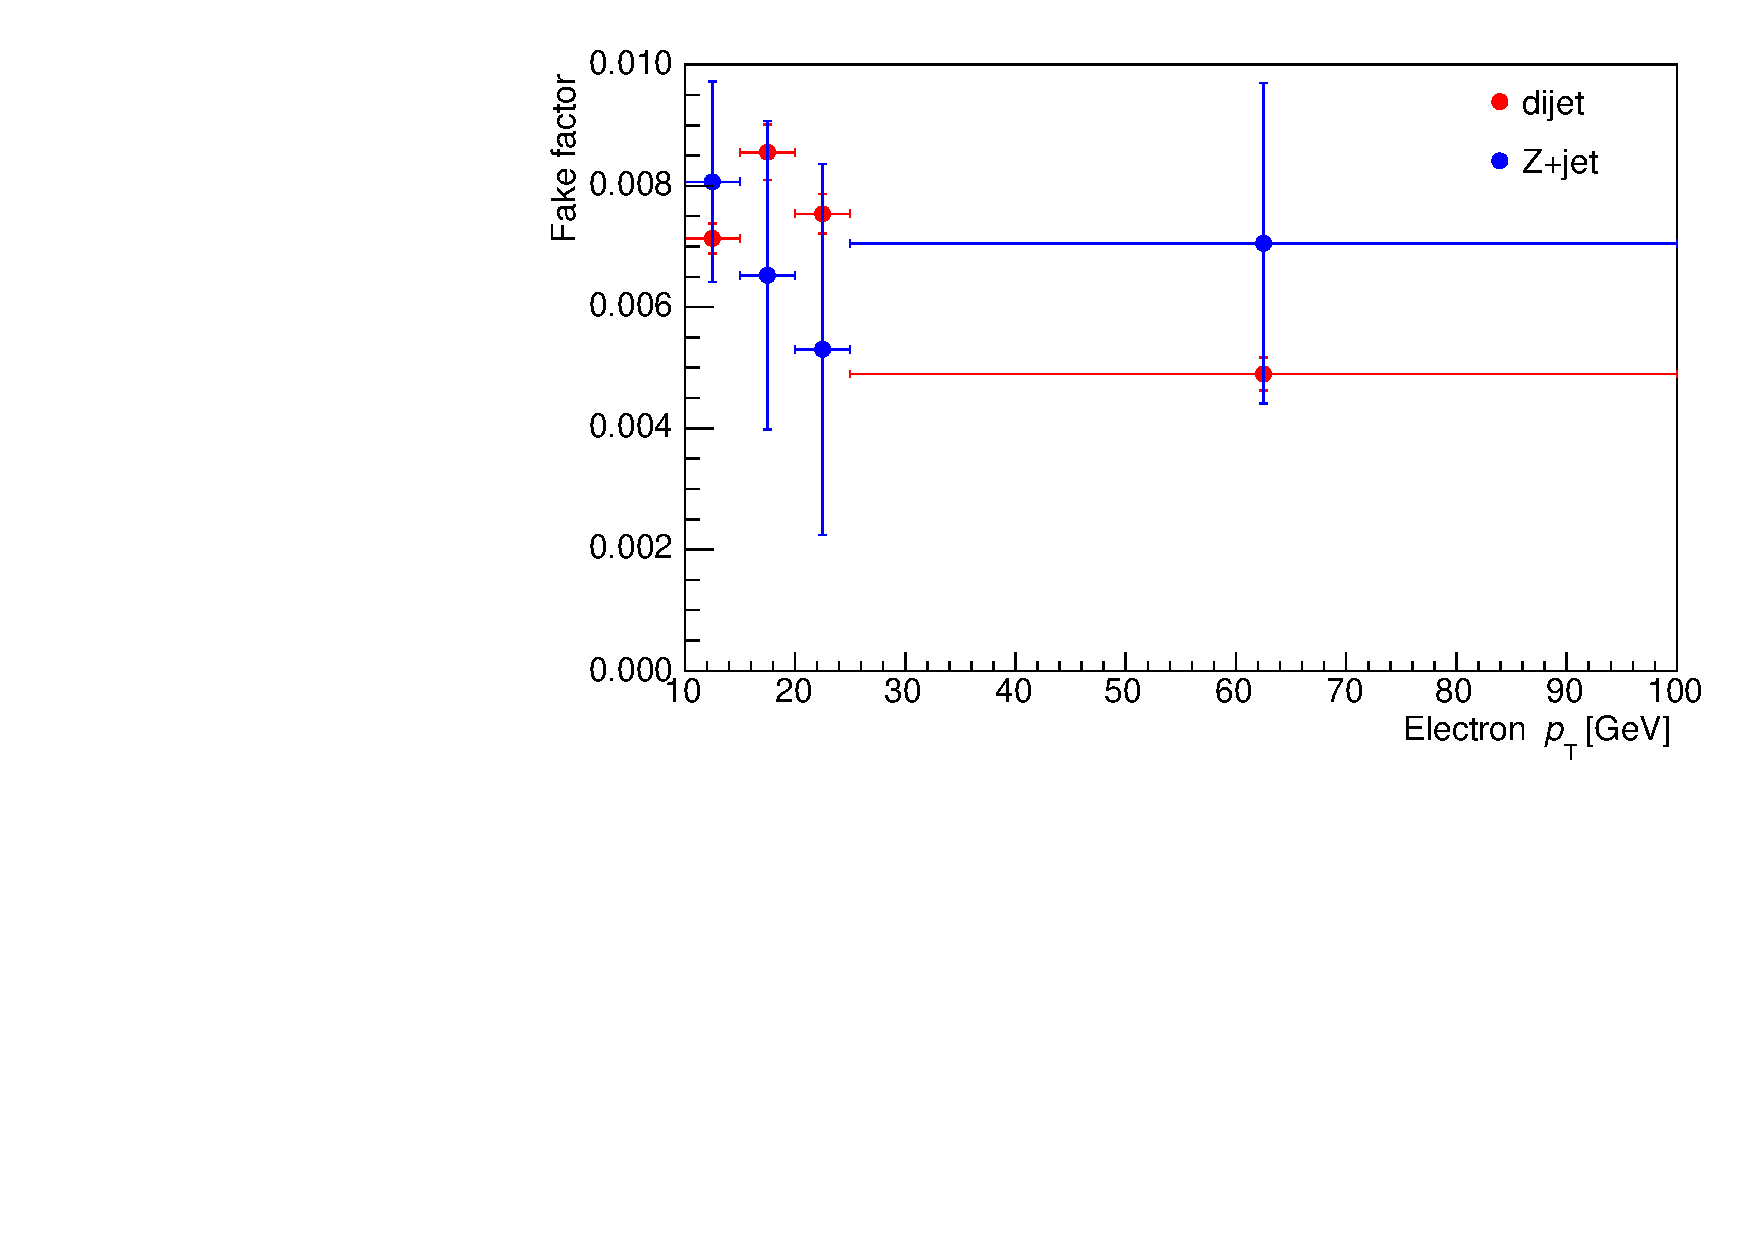
\includegraphics[width=0.495\textwidth]{custom_images/wjets/ff_el_data}
	\hfill
	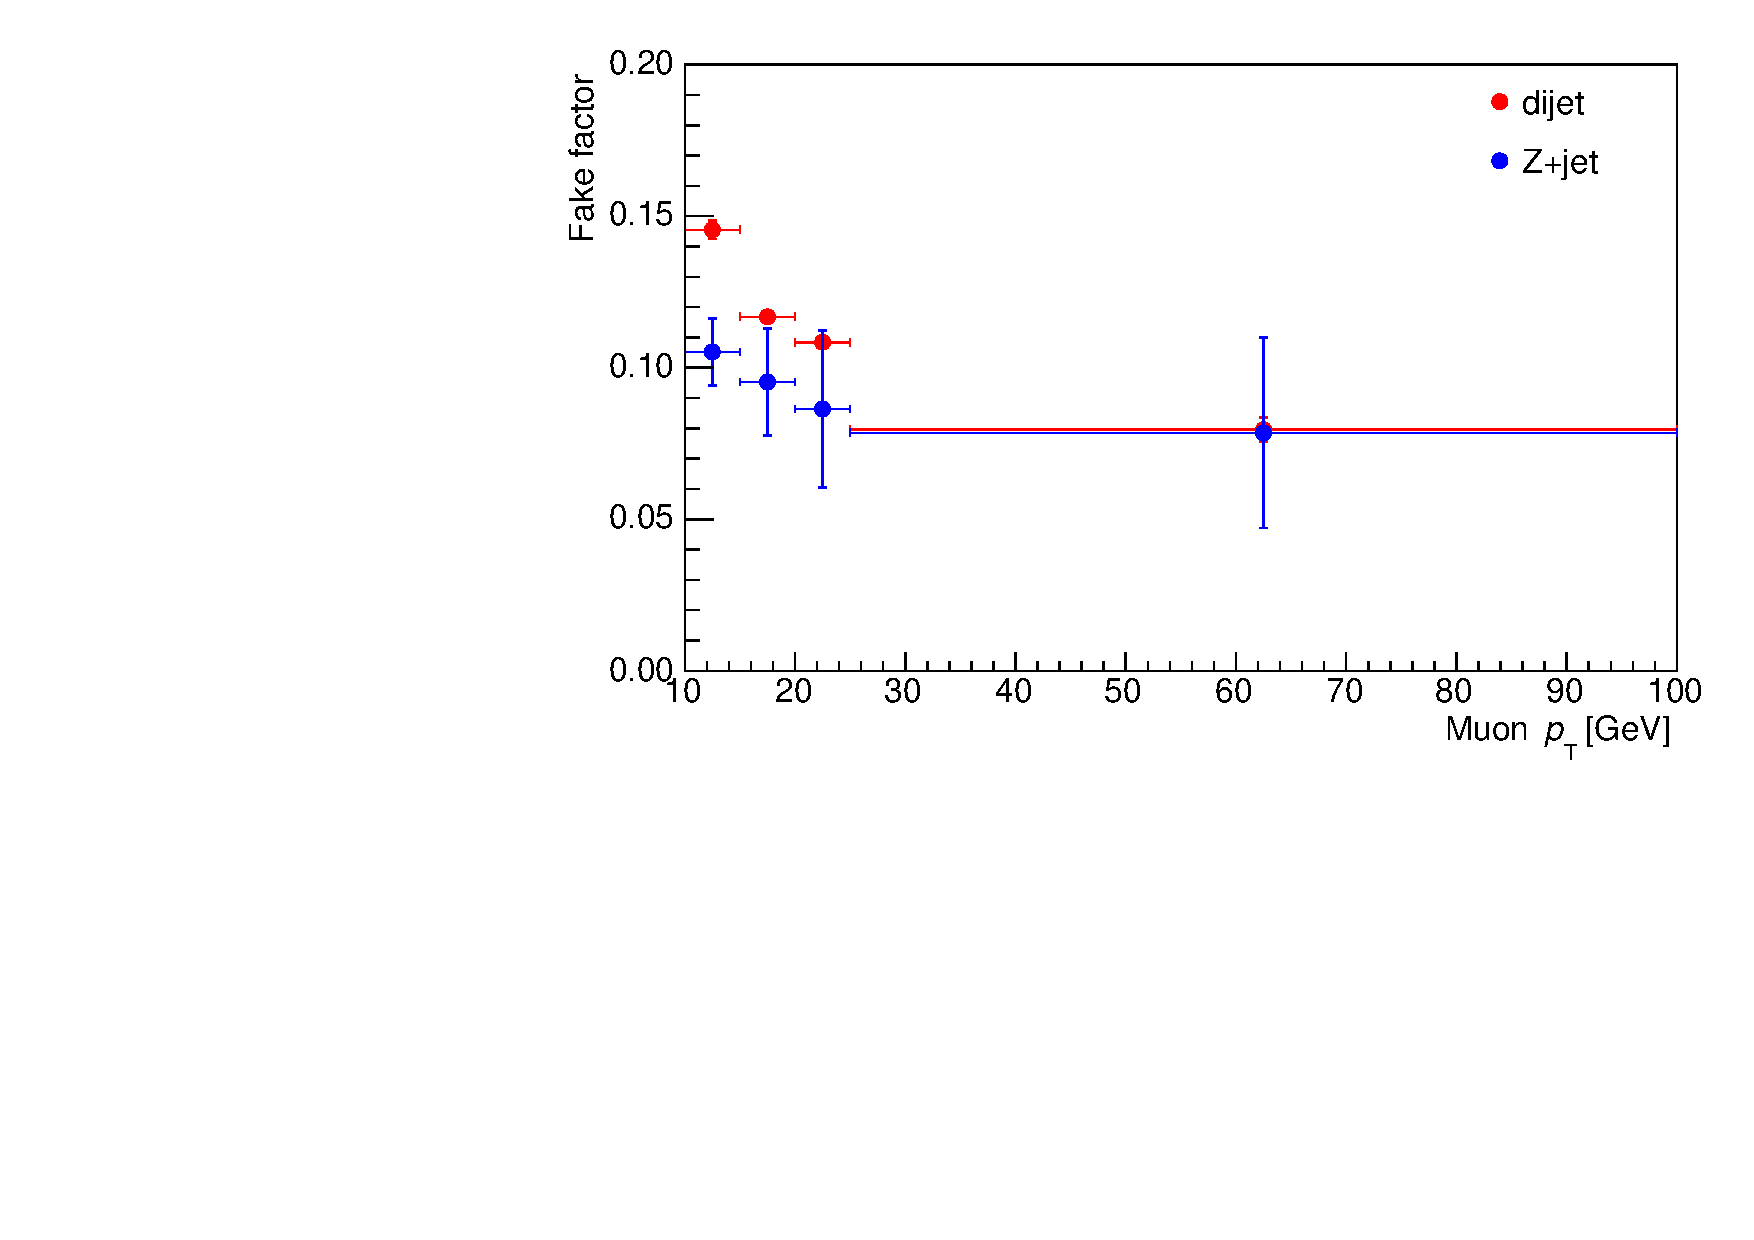
\includegraphics[width=0.495\textwidth]{custom_images/wjets/ff_mu_data}
	\caption{The fake factor measured in dijet (red) and \Zjets (blue) events versus \pt, 
	for electrons (left) and muons (right). The error bars include statistical 
	uncertainties and uncertainties in the background subtraction.}
	\label{fig:wjets:ff_data}
\end{figure}



\subsection{\Zjets fake factor measurement}
\label{sec:wjets:zjet_ff}

\textit{In situ} fake factor measurements are also made using \Zjets events. This 
involves counting the numbers of \id{\Plepton} and \antiid{\Plepton} objects in a \Zjets 
control region (CR), subtracting the expected prompt leptons and photon conversions from 
electroweak contamination (\Zgamma, \ZZ, \Zgstar, \WZ, \Wgstar), and calculating their 
ratio $f_{\Plepton} = N_{\id{\Plepton}} / N_{\antiid{\Plepton}}$.

Following data quality requirements, events are selected using unprescaled lepton 
triggers. This is possible because the triggered object is a lepton from the \PZ boson 
decay, and the \pt threshold can therefore be relatively high. In the $f_{\Pe}$ 
measurement, the \verb|EF_e24vhi_medium1| and \verb|EF_e60_medium1| triggers support 
\unit{$\pt > 25$}{\GeV}. In the $f_{\Pmu}$ measurement, the \verb|EF_mu24i_tight| and 
\verb|EF_mu36_tight| triggers are used with the dilepton \verb|EF_mu18_tight_mu8_EFFS| 
trigger to support \unit{$\pt > 22$}{\GeV}. The trigger naming scheme is explained in the 
caption of \Table~\ref{tab:sel:triggers}.

The \Zjets CR requires a pair of same-flavour and oppositely charged \id{\Plepton} objects 
to reconstruct the \PZ boson mass, \unit{$81 < \mll < 107$}{\GeV}. These leptons are 
excluded from the $f_{\Plepton}$ calculation. Electroweak contamination is suppressed by 
cuts on additional \id{\Plepton} and \antiid{\Plepton} objects: \ZZ is rejected by a veto 
on \unit{$76 < \mll < 107$}{\GeV} and \WZ is rejected by \unit{$\mtw < 30$}{\GeV}. Residual 
diboson backgrounds (\Zgamma, \ZZ, \Zgstar, \WZ, \Wgstar) are subtracted using MC 
predictions.

The measured electron and muon fake factors are shown in \Figure~\ref{fig:wjets:ff_data}. 
The uncertainty is dominated by statistical uncertainty. For this reason, 
$f_{\Plepton}^{\text{data,\Zjets}}$ is measured as a function of \pt only, and the $\eta$ 
dependence is injected from $f_{\Plepton}^{\text{data,dijet}}$. The uncertainty due to 
electroweak subtraction is also significant (estimated by varying the diboson cross 
sections by 10\%), because the contamination to the \Zjets CR is not negligible. Although 
$f_{\Plepton}^{\text{data,\Zjets}}$ has larger uncertainties than 
$f_{\Plepton}^{\text{data,dijet}}$, it shall be used in the \Wjets background estimation. 
This is because jets in \Zjets and \Wjets events are expected to have similar flavour 
composition, and therefore similar fake factors (see \Section~\ref{sec:wjets:wjet_bkg}).



\subsection{\Wjets background estimation}
\label{sec:wjets:wjet_bkg}

The \Wjets background to the opposite-sign (OS) and same-sign (SS) dilepton samples are 
estimated from the \Wjets control sample, using (\ref{eq:wjet_bkgto_dilepton}). The 
\Wjets control sample $\mathcal{N}_{\id{\Plepton}\antiid{\Plepton}}$ contains events with 
one ID lepton and one anti-ID lepton, selected from events passing the data data quality 
criteria and triggers specified in \Section~\ref{sec:selection}. Generally, it is the 
lepton from the \PW boson decay that fires the single lepton triggers. Contamination is 
small, and is estimated by the fake factor method for dijet events (see 
\Section~\ref{sec:wjets:dijet_bkg}) and MC for other processes.

The fake factor of a process is determined by the jet flavour composition of that 
process. This is because the fake factor of each hadron flavour is independent of 
the hard scatter. Specifically, $f_{\Pe}$ is larger for heavy flavour because the electron 
particle identification is tuned to reject light flavour jets, and $f_{\Pmu}$ is larger 
for light flavour because the $d_0$ criterion suppresses long-lived heavy flavour hadrons.

Since we use OS and SS samples, it is useful to consider the jet flavour composition of 
the \Wjets process in each sample. There are diagrams like \HepProcess{\Pquark\Pgluon 
\HepTo \PW\Pquark'}, where the outgoing quark has OS charge to the \PW boson (\eg 
\HepProcess{\PW + \Pcharm}),\footnote{
	It should be emphasised that \HepProcess{\Pquark\Pgluon \HepTo \PW+\Pbottom} is highly 
	suppressed by the near unity of $V_{\Ptop\Pbottom}$	in the CKM matrix and the negligible
	top contribution to the incoming PDFs.
} 
and there are diagrams like \HepProcess{\Pquark\APquark' 
\HepTo \PW\Pgluon}, where the gluon subsequently splits to a \HepProcess{\Pquark\APquark} 
pair (\eg \HepProcess{\PW + \Pbottom\APbottom}). Therefore, in terms of the \PW and quark 
charges, the former diagrams contribute to OS only and the latter contribute to OS and 
SS equally. However, the samples are categorised according to the signs of the leptons, 
and so the extent to which the quark charge is preserved in the reconstructed lepton is 
important. When a hadron decays leptonically, its sign is preserved in the lepton. 
Without such a non-prompt lepton, the sign of the jet charge is more likely to be inverted 
in the reconstructed lepton. In the case of photon conversions from \HepProcess{\Ppizero 
\HepTo \Pphoton\Pphoton}, there is no asymmetry. Thus, considering the above points, there 
is a strong OS/SS asymmetry in \Pcharm-jets, a mild asymmetry in light flavour jets, and no 
asymmetry in \Pbottom-jets and \HepProcess{\Ppizero \HepTo \Pphoton\Pphoton} (see 
\Figure~\ref{fig:wjets:flav_comp}).

\begin{figure}[t]
	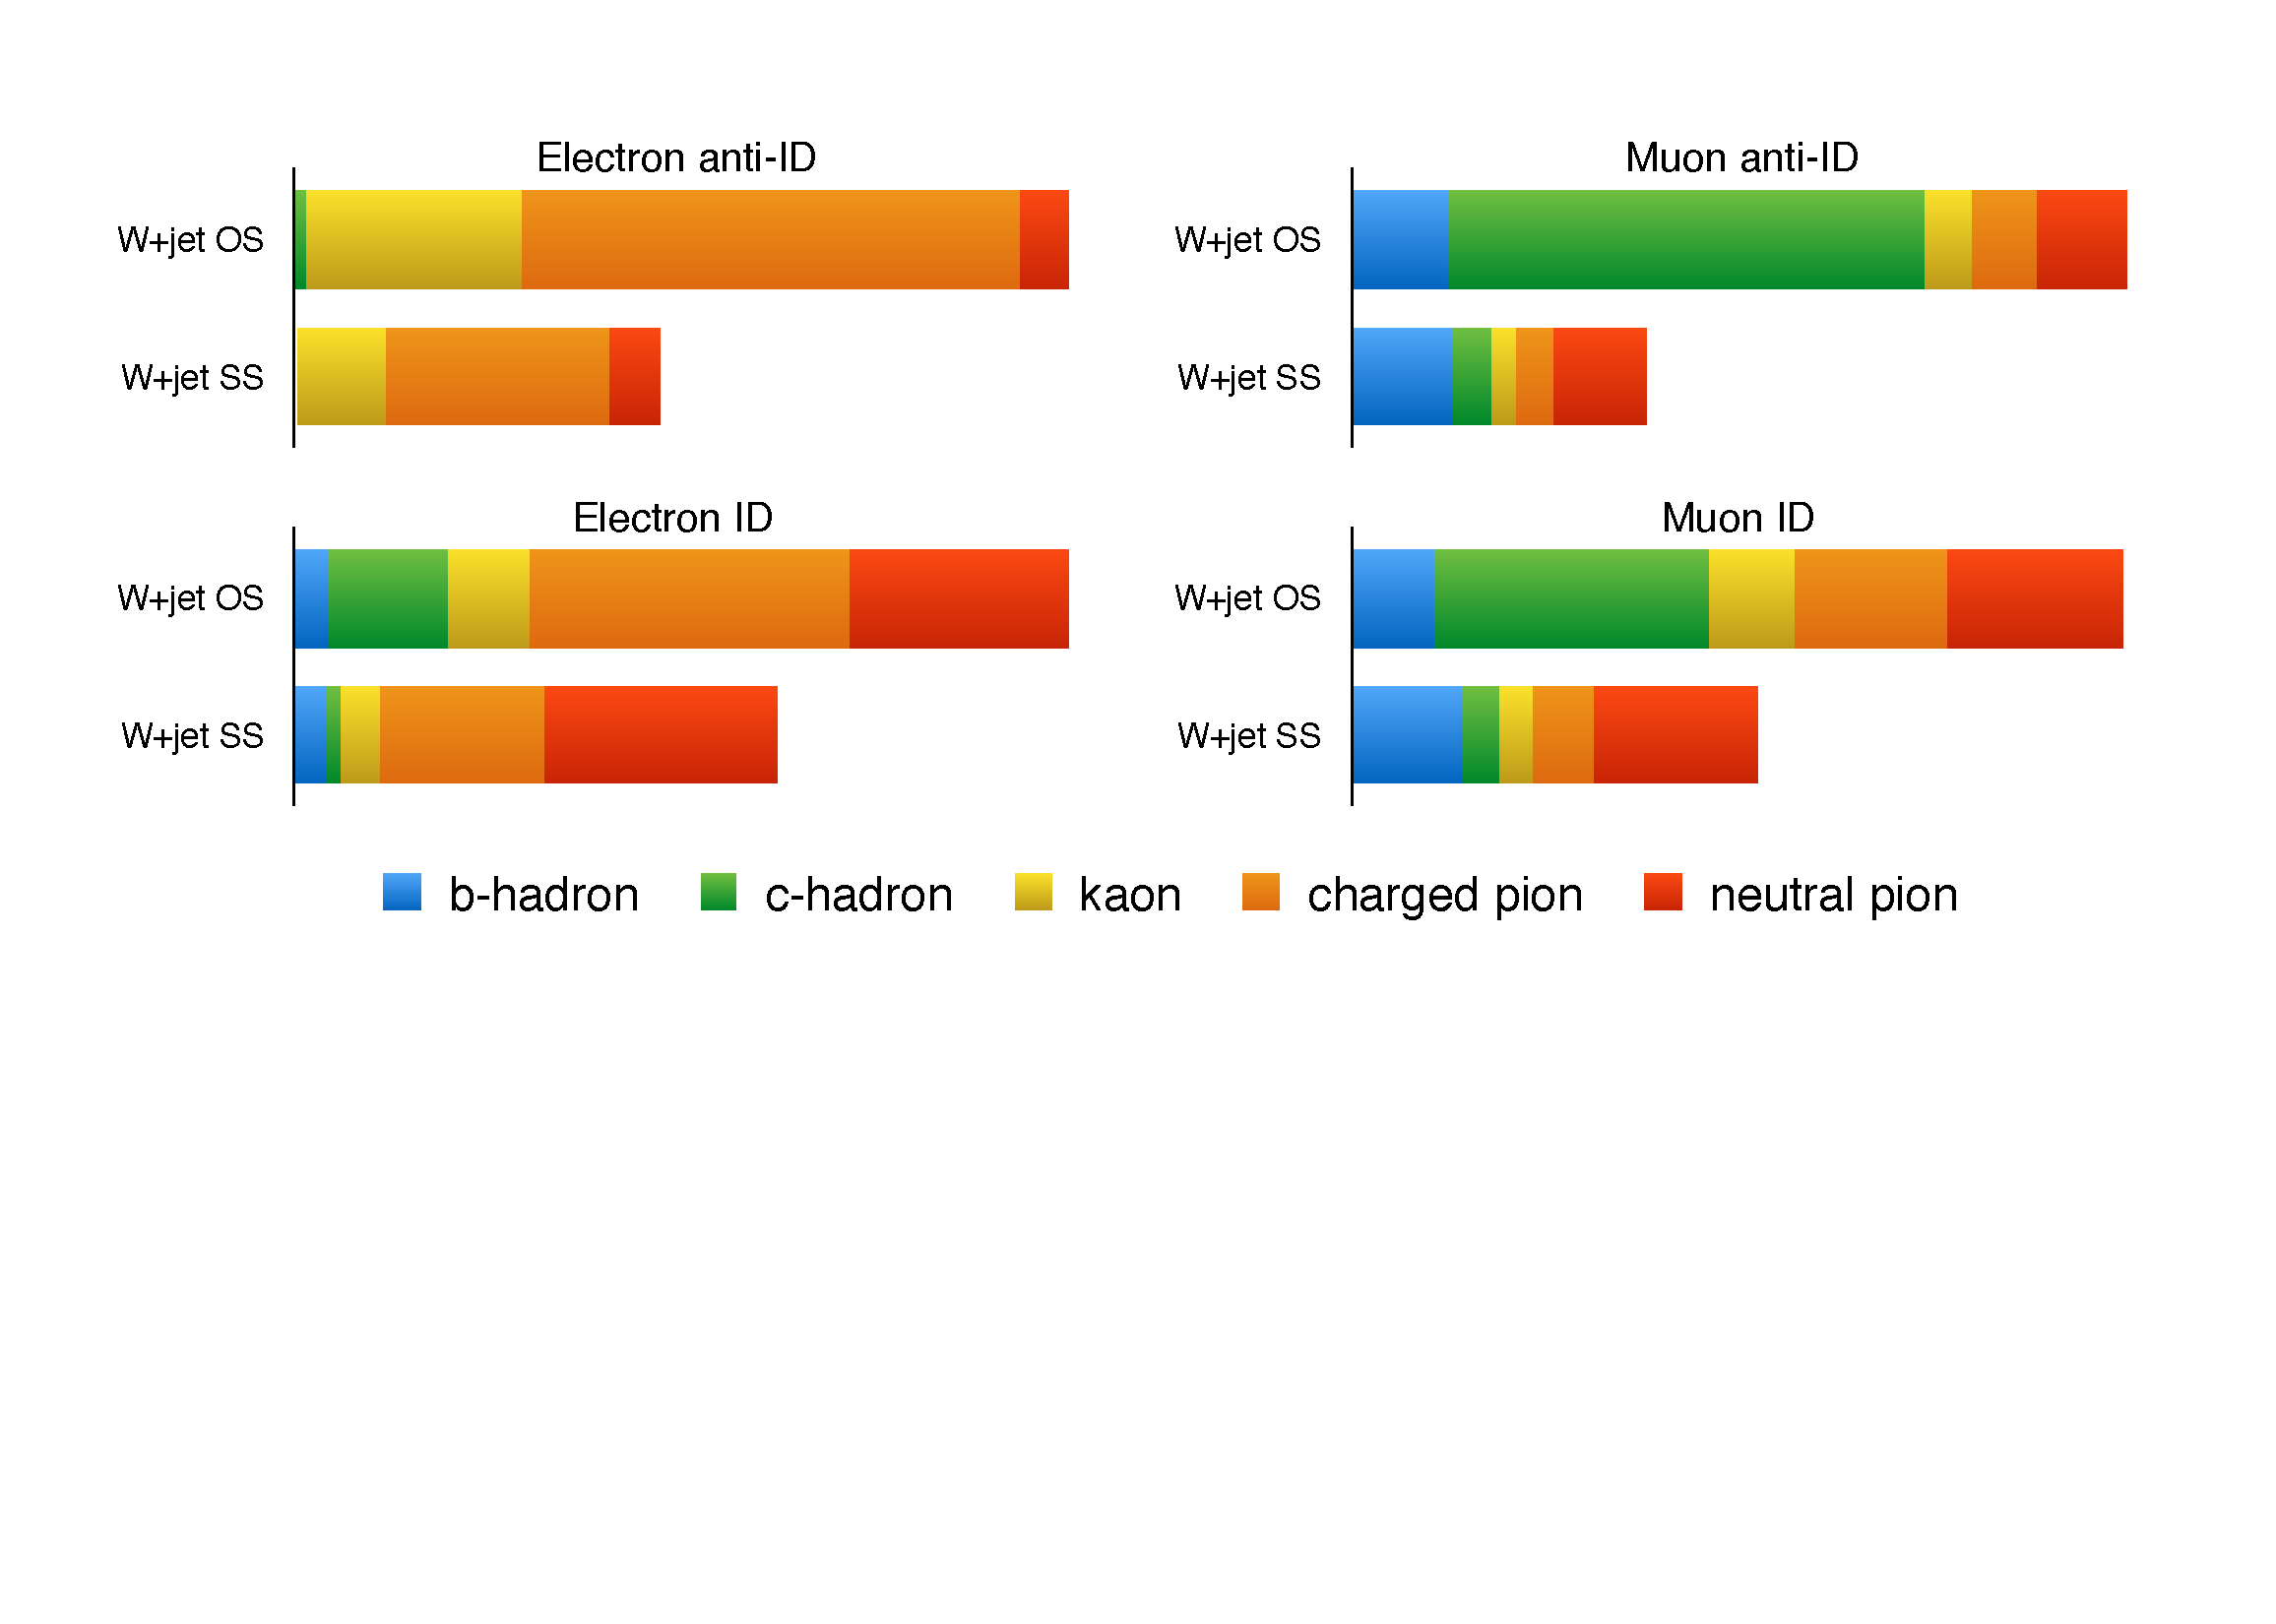
\includegraphics[width=\textwidth,clip=true,trim=1.8cm 12cm 2cm 2cm]{custom_images/wjets/wjets_flavcomp}
	\caption{The jet flavour composition of fake leptons, for opposite-sign (OS) and 
	same-sign (SS) \Wjets events. Each SS axis is normalised to the corresponding OS 
	axis.}
	\label{fig:wjets:flav_comp}
\end{figure}

MC-based corrections are applied to the measured \Zjets fake factor in order to account 
for the different jet flavour compositions of the OS and SS \Wjets processes
\begin{equation}
	f_{\Plepton,i}^{\text{pred,\Wjets}}\parenths{\pt,\eta} &= f_{\Plepton}^{\text{data,\Zjets}}\parenths{\pt} \cdot \frac{f_{\Plepton}^{\text{data,dijet}}\parenths{\pt, \eta}}{f_{\Plepton}^{\text{data,dijet}}\parenths{\pt}} \cdot \frac{f_{\Plepton,i}^{\text{MC,\Wjets}}}{f_{\Plepton}^{\text{MC,\Zjets}}}
	\label{eq:wjet_ff}
\end{equation}
where $i = \text{OS, SS}$. The injection of $\eta$-dependence from the dijet fake factor 
is also shown in (\ref{eq:wjet_ff}). The \Zjets fake factor is used because \Zjets has a 
similar jet flavour composition to \Wjets. The correction factors are derived with 
\meps{\alpgen}{\pythia{6}}, and compared to those of \meps{\alpgen}{\fherwig} and 
\meps{\powhegbox}{\pythia{8}} to obtain a systematic uncertainty. The corrections factors 
are \statsyst{0.99}{0.05}{0.19} for OS electrons, \statsyst{1.00}{0.08}{0.21} for OS 
muons, \statsyst{1.25}{0.08}{0.30} for SS electrons and \statsyst{1.40}{0.14}{0.47} for 
SS muons.

The \Wjets background is dominated by uncertainties in the fake factor. These are split 
into components that are correlated and uncorrelated between 
$f_{\text{\Plepton,OS}}^{\text{\Wjets}}$ and $f_{\text{\Plepton,SS}}^{\text{\Wjets}}$. 
Components correlated between OS and SS largely cancel in the same-sign control region 
method of estimating the non-\WW diboson background (see \Section~\ref{sec:diboson:sscr}). 
This method also offers validation of the the \Wjets background estimation.



\subsection{Dijet background estimation}
\label{sec:wjets:dijet_bkg}

The dijet backgrounds to the dilepton and \Wjets samples are estimated from the dijet 
control sample, using (\ref{eq:dijet_bkgto_dilepton}) and (\ref{eq:dijet_bkgto_wjet}) 
respectively. The dijet control sample $\mathcal{N}_{\antiid{\Plepton}\antiid{\Plepton}}$ 
contains events with two anti-ID leptons, selected from events passing the data quality 
criteria and triggers specified in \Section~\ref{sec:selection}. They are accepted by the 
dilepton triggers since these have looser lepton selections. Contamination from \Wjets and 
other processes is estimated with MC, though is generally small.

The dijet fake factor $f_{\Plepton}^{\text{data,dijet}}$ is measured in events containing 
a balancing jet (passing the offline jet selection). However, in 
(\ref{eq:dijet_bkgto_dilepton}) and (\ref{eq:dijet_bkgto_wjet}) the fake factors are 
applied to events containing another anti-ID lepton 
($f_{\Plepton \vert \antiid{\Plepton}}^{\text{pred,dijet}}$), or as if there is an ID lepton
in the event ($f_{\Plepton \vert \id{\Plepton}}^{\text{pred,dijet}}$). This can heavily 
bias the jet flavour composition of the selected events, and this in turn can affect the 
fake factor of interest. For example, if the other object is a muon, this increases the 
probability that the event contains heavy flavour jets. Consequently, $f_{\Pe}$ would 
increase and $f_{\Pmu}$ would decrease (see \Section~\ref{sec:wjets:wjet_bkg}).

MC-based corrections are applied to the measured dijet fake factor in order to account 
for the correlation between $f_{\Plepton}$ and the other object in the event
\begin{equation}
	f_{\Plepton \vert \antiid{\Plepton}}^{\text{pred,dijet}}\parenths{\pt,\eta} &= f_{\Plepton}^{\text{data,dijet}}\parenths{\pt,\eta} \cdot \frac{f_{\Plepton \vert \antiid{\Plepton}}^{\text{MC,dijet}}}{f_{\Plepton \vert j}^{\text{MC,dijet}}} \\
	f_{\Plepton \vert \id{\Plepton}}^{\text{pred,dijet}}\parenths{\pt,\eta} &= f_{\Plepton}^{\text{data,dijet}}\parenths{\pt,\eta} \cdot \frac{f_{\Plepton \vert \id{\Plepton}}^{\text{MC,dijet}}}{f_{\Plepton \vert j}^{\text{MC,dijet}}} \,.
\end{equation}

The dijet background has a very small contribution to the \HWW signal regions, but has 
large uncertainties dominated by the MC-based corrections. It is difficult to define a 
high purity dijet validation region in the dilepton sample, though good agreement with 
experimental data is observed in the low \met regions where this background is enhanced.


\section{Non-\WW diboson}
	\label{sec:diboson}
	%!TEX root = ../../thesis.tex

The non-\WW diboson background comprises the \Wgamma, \Wgstar, \WZ and \ZZ processes (in 
order of contribution to the signal region). \Wgamma events feature a prompt photon that 
passes the electron selection, via an asymmetric conversion (\epluseminus production). The 
other processes have signatures of \HepProcess{\Plepton\Pnu\Plepton\Plepton}, 
\HepProcess{\Plepton\Plepton\Plepton\Plepton} or \HepProcess{\Plepton\Plepton\Pnu\Pnu}, and 
usually contribute when one or more leptons fail object selection (\eg 
\unit{$\pt < 10$}{\GeV} or $\mods{\eta} > 2.5$).



\subsection{Same-sign control region}
\label{sec:diboson:sscr}

In non-\WW diboson backgrounds, a symmetry is expected to exist between opposite-sign (OS) 
and same-sign (SS) dilepton events; this is particularly true in the \emch/\mech channels, 
where asymmetric final states are removed. Conversely, the \WW, top and \DY backgrounds 
only contribute to the OS sample. Finally, the \Wjets background displays a partial OS/SS 
symmetry, as described in \Section~\ref{sec:wjets:wjet_bkg}. Thus, SS events can be used to 
estimate the non-\WW diboson background in the OS signal region, whilst validating the 
\Wjets estimation.

An SS control region (CR) is defined using identical criteria to the OS signal region (SR). 
In the language of \Section~\ref{sec:wjets}, the SS CR events are in the SR of the 
$\mathcal{N}_{\id{\Plepton}\id{\Plepton}\text{,SS}}$ sample. This is used to determine the 
normalisation of the non-\WW diboson background, whilst the shapes of observables used in 
the fitting procedure (\ie \mt, \mll and \ptsubleadlep) are modelled by MC. This is 
equivalent to
\begin{equation}
	N_{\HepProcess{\PV\PV}}^{\text{pred,SR}} &= \alpha_{\HepProcess{\PV\PV}} \cdot \parenths{N^{\text{data,CR}} - N_{\text{non-}\HepProcess{\PV\PV}}^{\text{pred,CR}}} \label{eq:sscr} \\
	\alpha_{\HepProcess{\PV\PV}} &= N_{\HepProcess{\PV\PV}}^{\text{MC,SR}} / N_{\HepProcess{\PV\PV}}^{\text{MC,CR}}
\end{equation}
where $\HepProcess{\PV\PV} = \Wgamma + \Wgstar + \WZ + \ZZ$ and 
$N_{\text{non-}\HepProcess{\PV\PV}}^{\text{pred,CR}}$ is dominated by \Wjets. The 
extrapolation $\alpha_{\HepProcess{\PV\PV}}$ represents the MC predictions for shapes of
observables, since the OS/SS symmetry implies that the total normalisation is unchanged. 

The SS CR method is only used in the 0-jet and 1-jet bins of the \emch/\mech channels, 
using a combined \emch{}+\mech channel to define the CR. All other signal regions use 
estimate the non-\WW diboson background using MC only.

Uncertainties in the normalisation of the constituent processes will cancel if the 
composition of the non-\WW diboson background is the same in SS and OS events; this is 
modelled by MC. However, uncertainties in the shapes of distributions remain, since these 
are not constrained by the SS CR method. Additionally, the uncertainty component of the OS 
\Wjets background that is correlated between OS and SS will cancel in the SS CR method; an 
increase in the SS \Wjets background will be compensated by a decrease in the non-\WW 
diboson background, and vice versa.

To estimate the non-\WW diboson background in regions other than the SR, the method is 
viewed as providing a simple data-driven normalisation factor. This is equivalent to 
neglecting the extrapolation uncertainties, but is helpful when plotting observables. The 
normalisation factors are measured to be \stat{0.96}{0.07} in the 0-jet bin and 
\stat{0.93}{0.13} in the 1-jet bin\todo{update}. 

\Figure~\ref{fig:sscr} validates the MC shape modelling of the fit observables in the SS 
CRs, following application of the normalisation factors. Good agreement with experimental 
data is observed. Note that these SS distributions are not directly used, since only the 
total number of events in the SS CRs are used in (\ref{eq:sscr}).

\begin{figure}[p]
	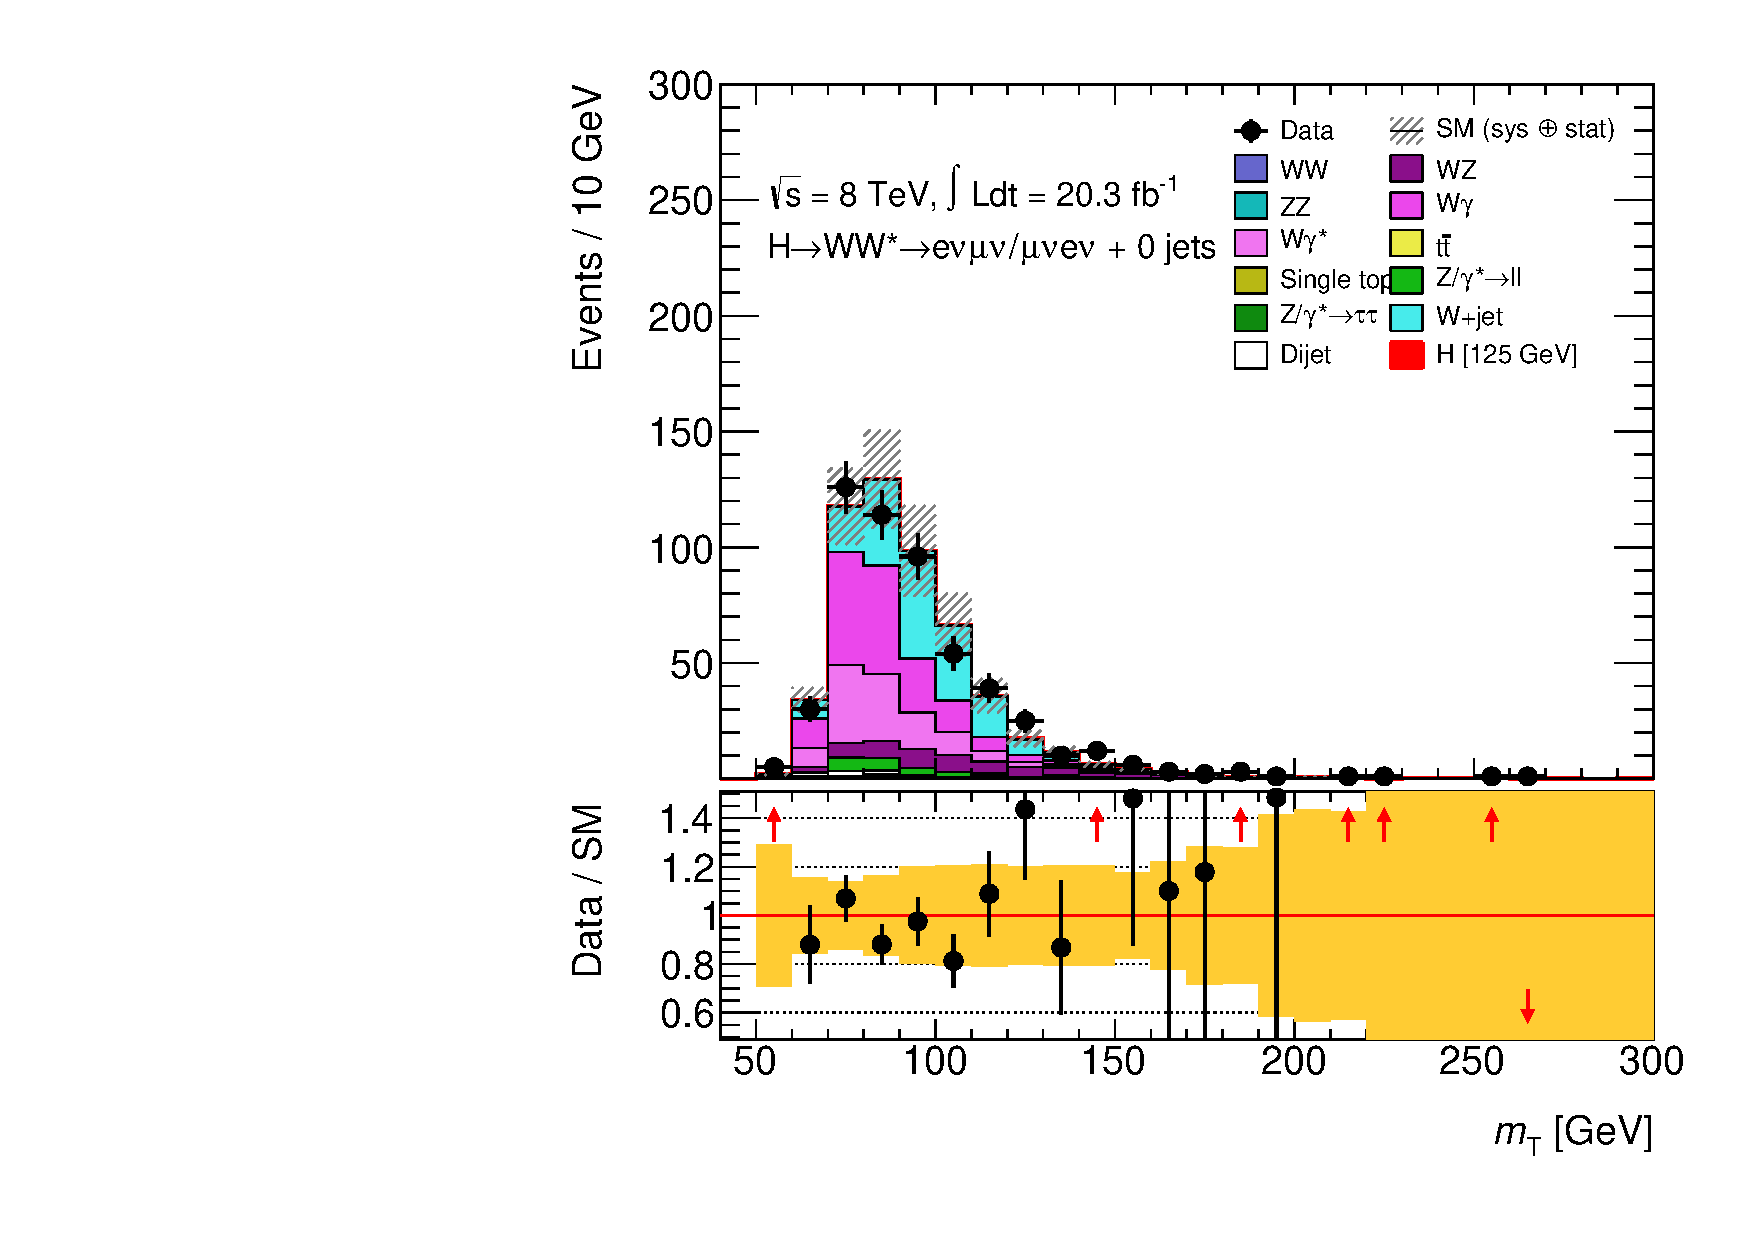
\includegraphics[width=0.48\textwidth]{tex/backgrounds/emme_CutFRecoil_0jet_sscr_MT_TrackHWW_Clj_mh125_lin}
	\hfill
	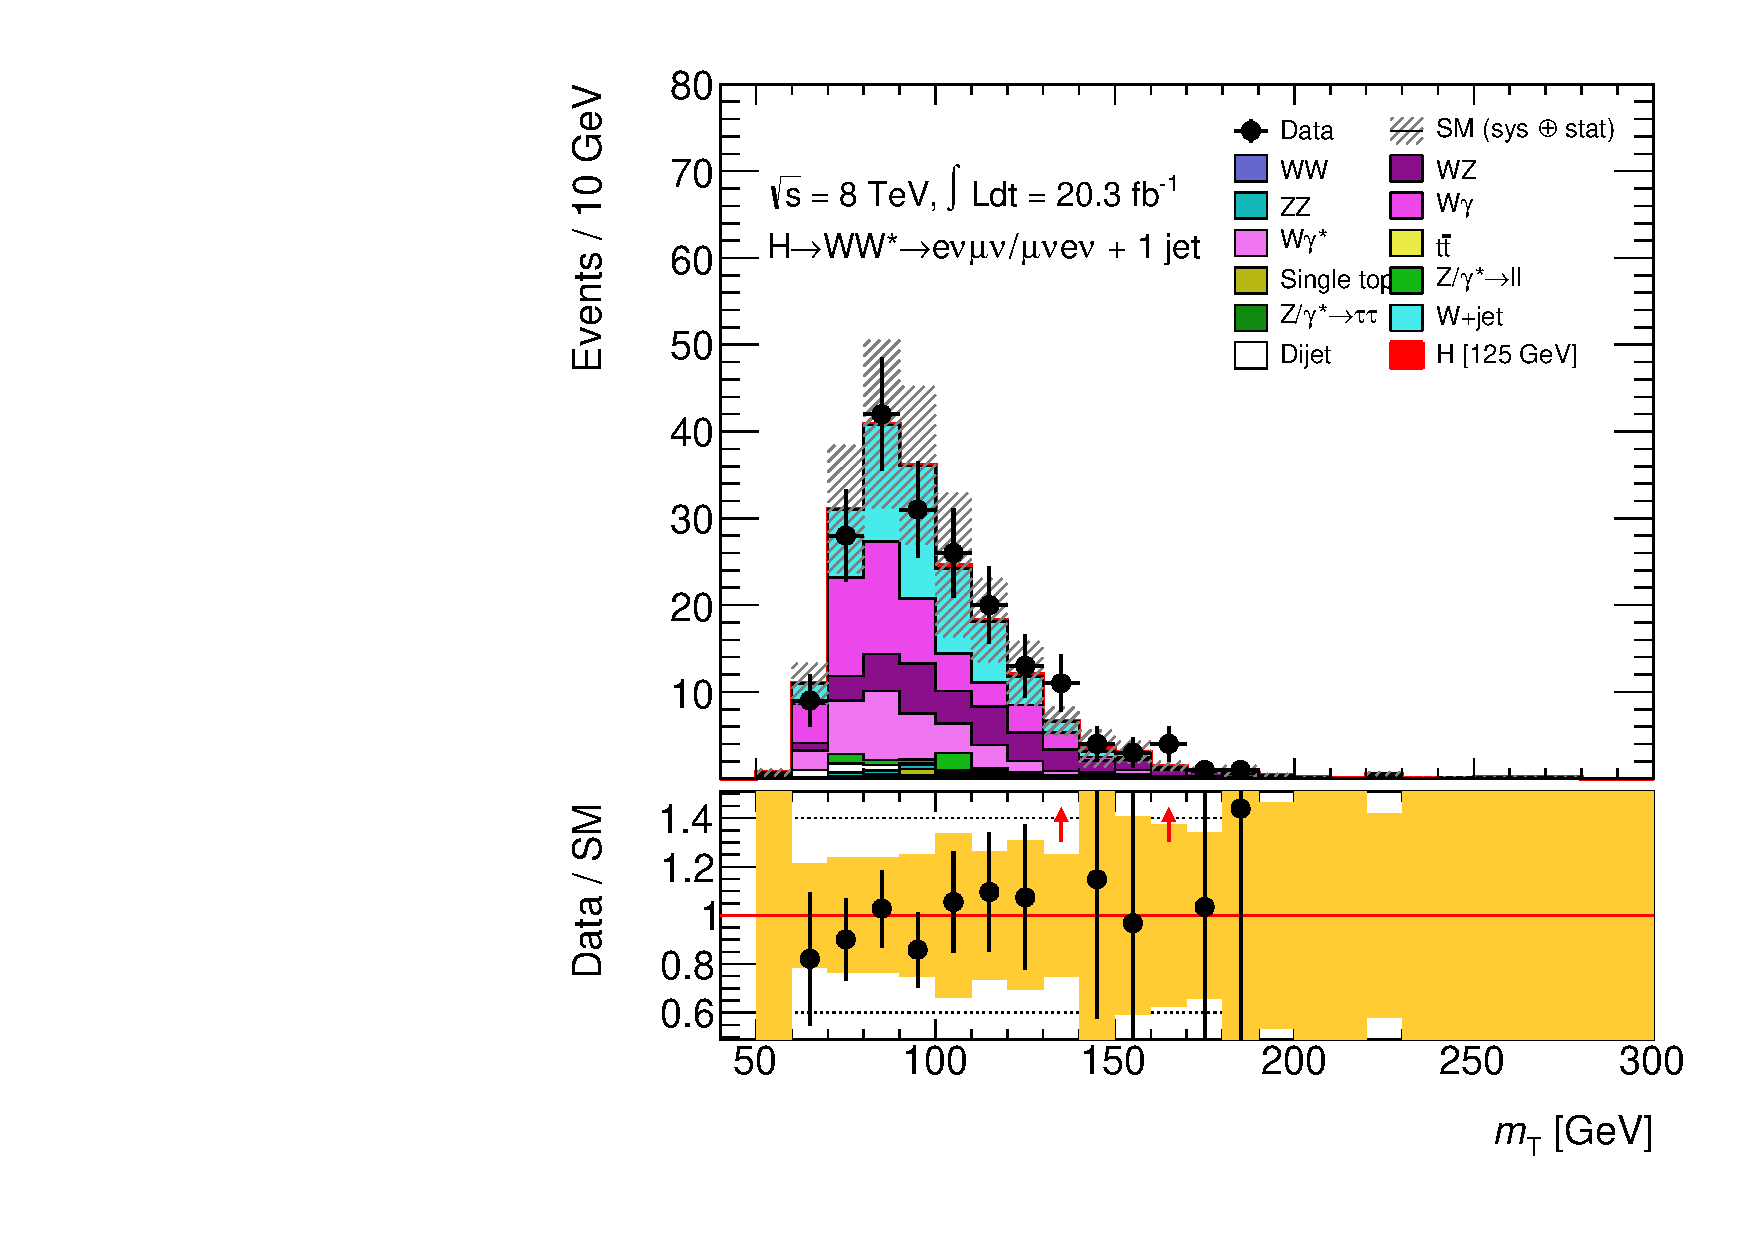
\includegraphics[width=0.48\textwidth]{tex/backgrounds/emme_CutFRecoil_1jet_sscr_MT_TrackHWW_Clj_mh125_lin}
	\\
	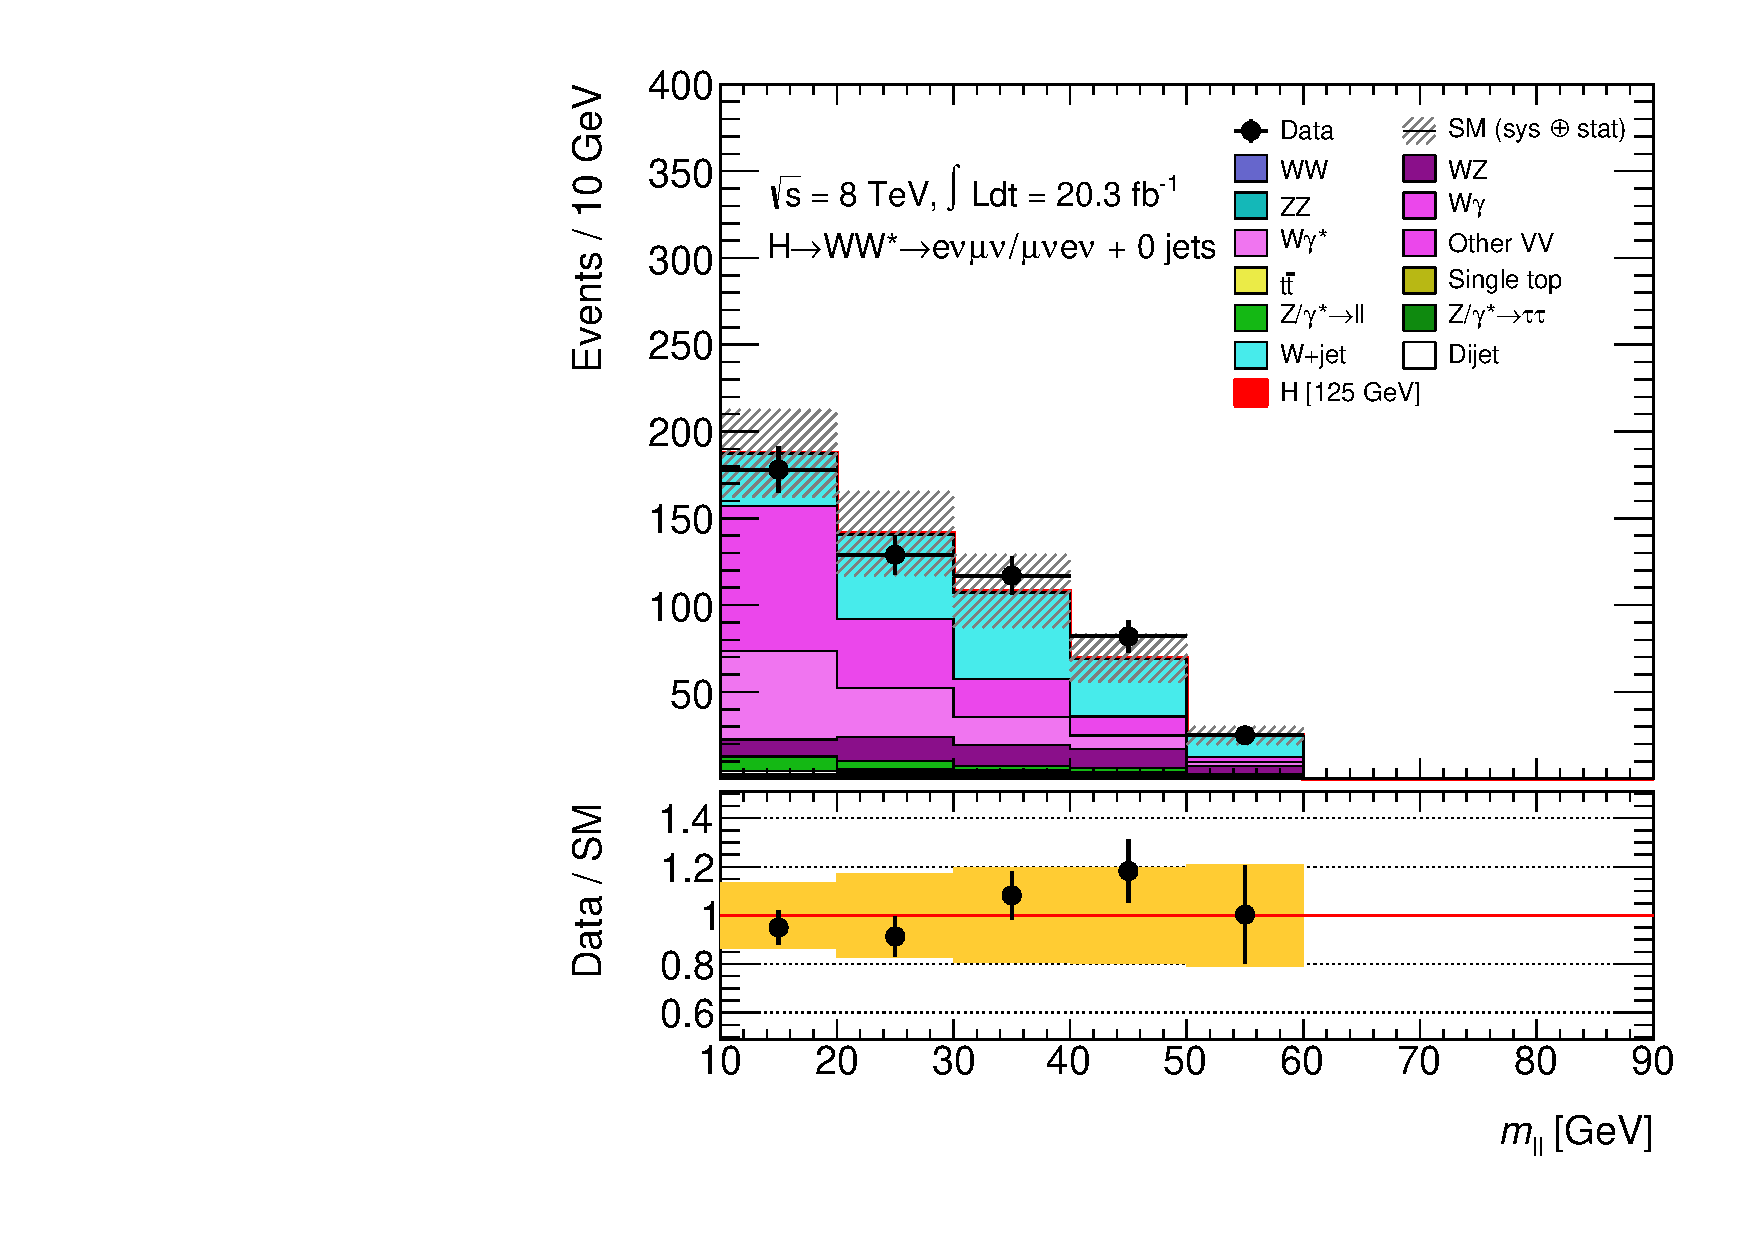
\includegraphics[width=0.48\textwidth]{tex/backgrounds/emme_CutFRecoil_0jet_sscr_Mll_zoom_mh125_lin}
	\hfill
	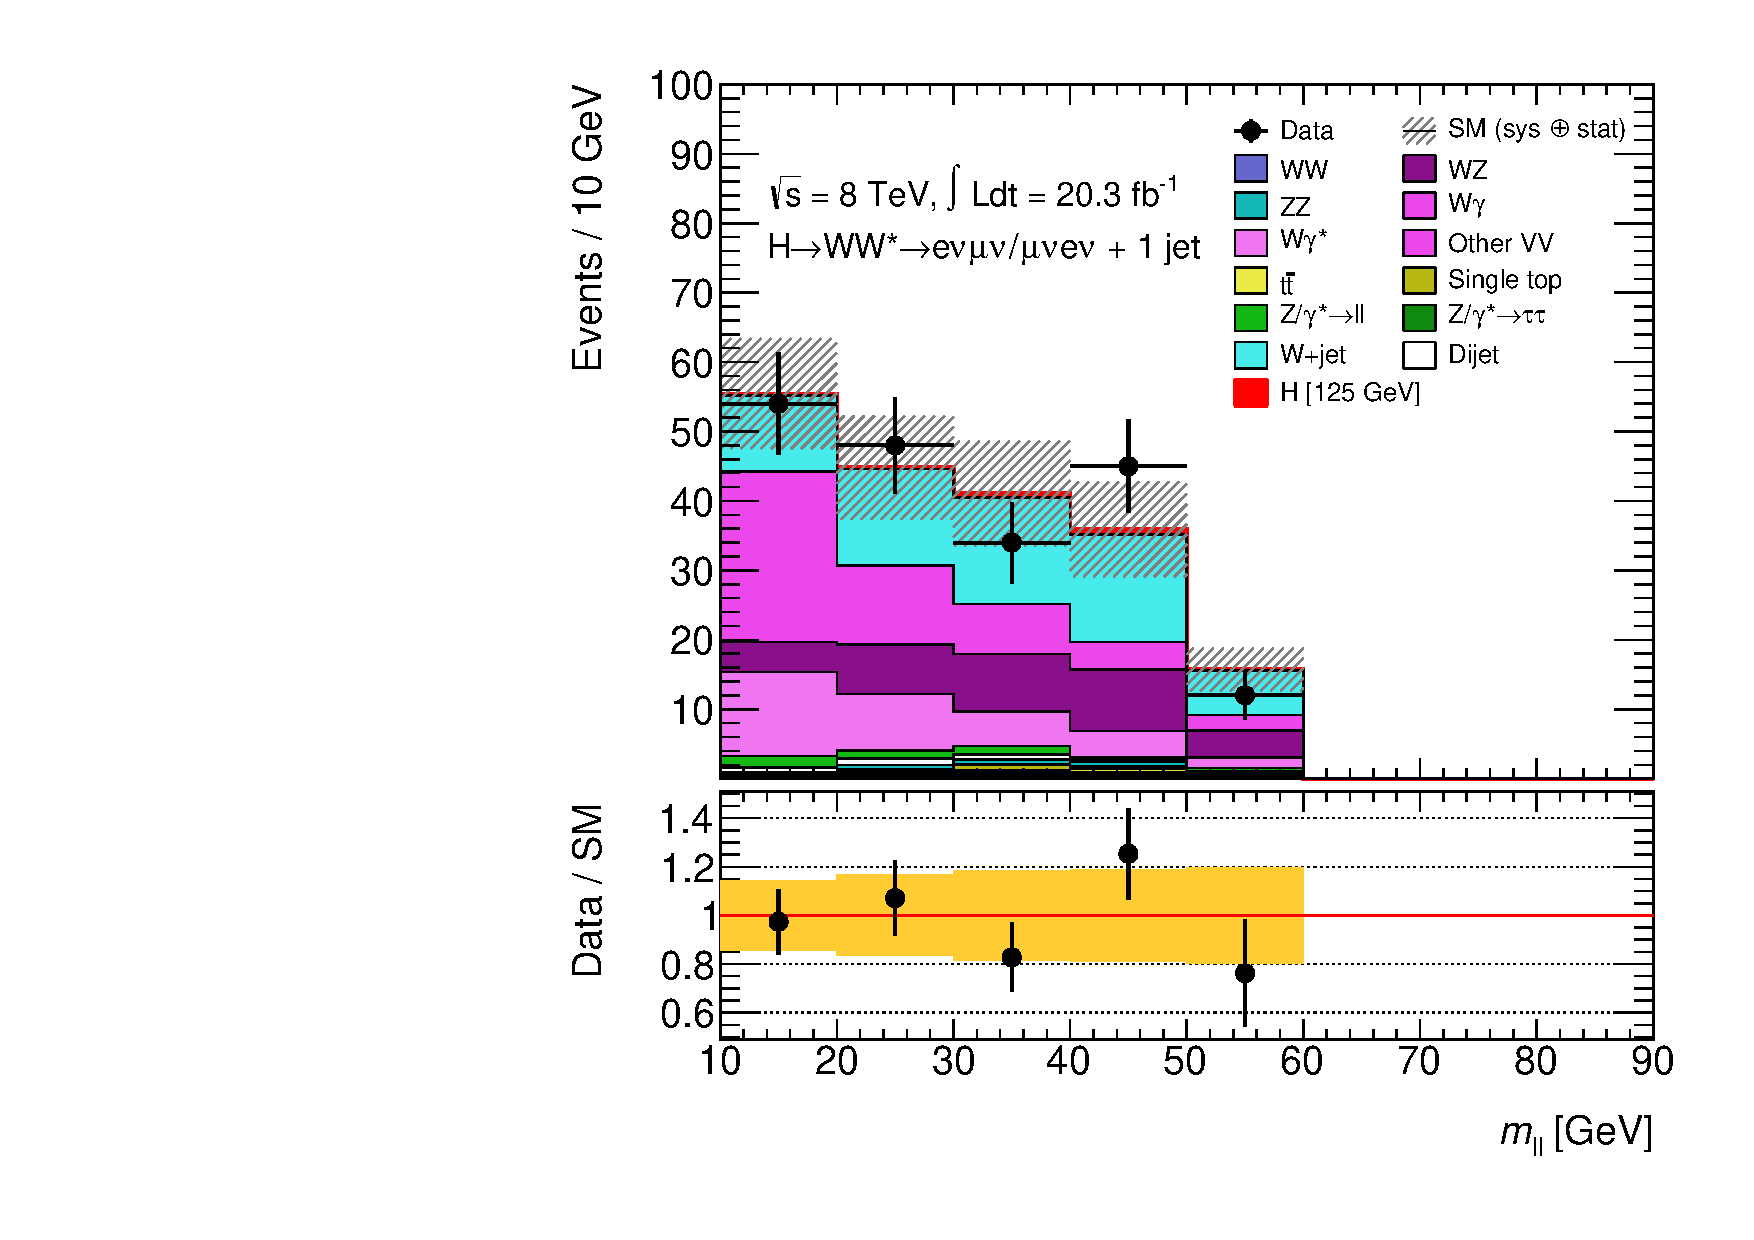
\includegraphics[width=0.48\textwidth]{tex/backgrounds/emme_CutFRecoil_1jet_sscr_Mll_zoom_mh125_lin}
	\\
	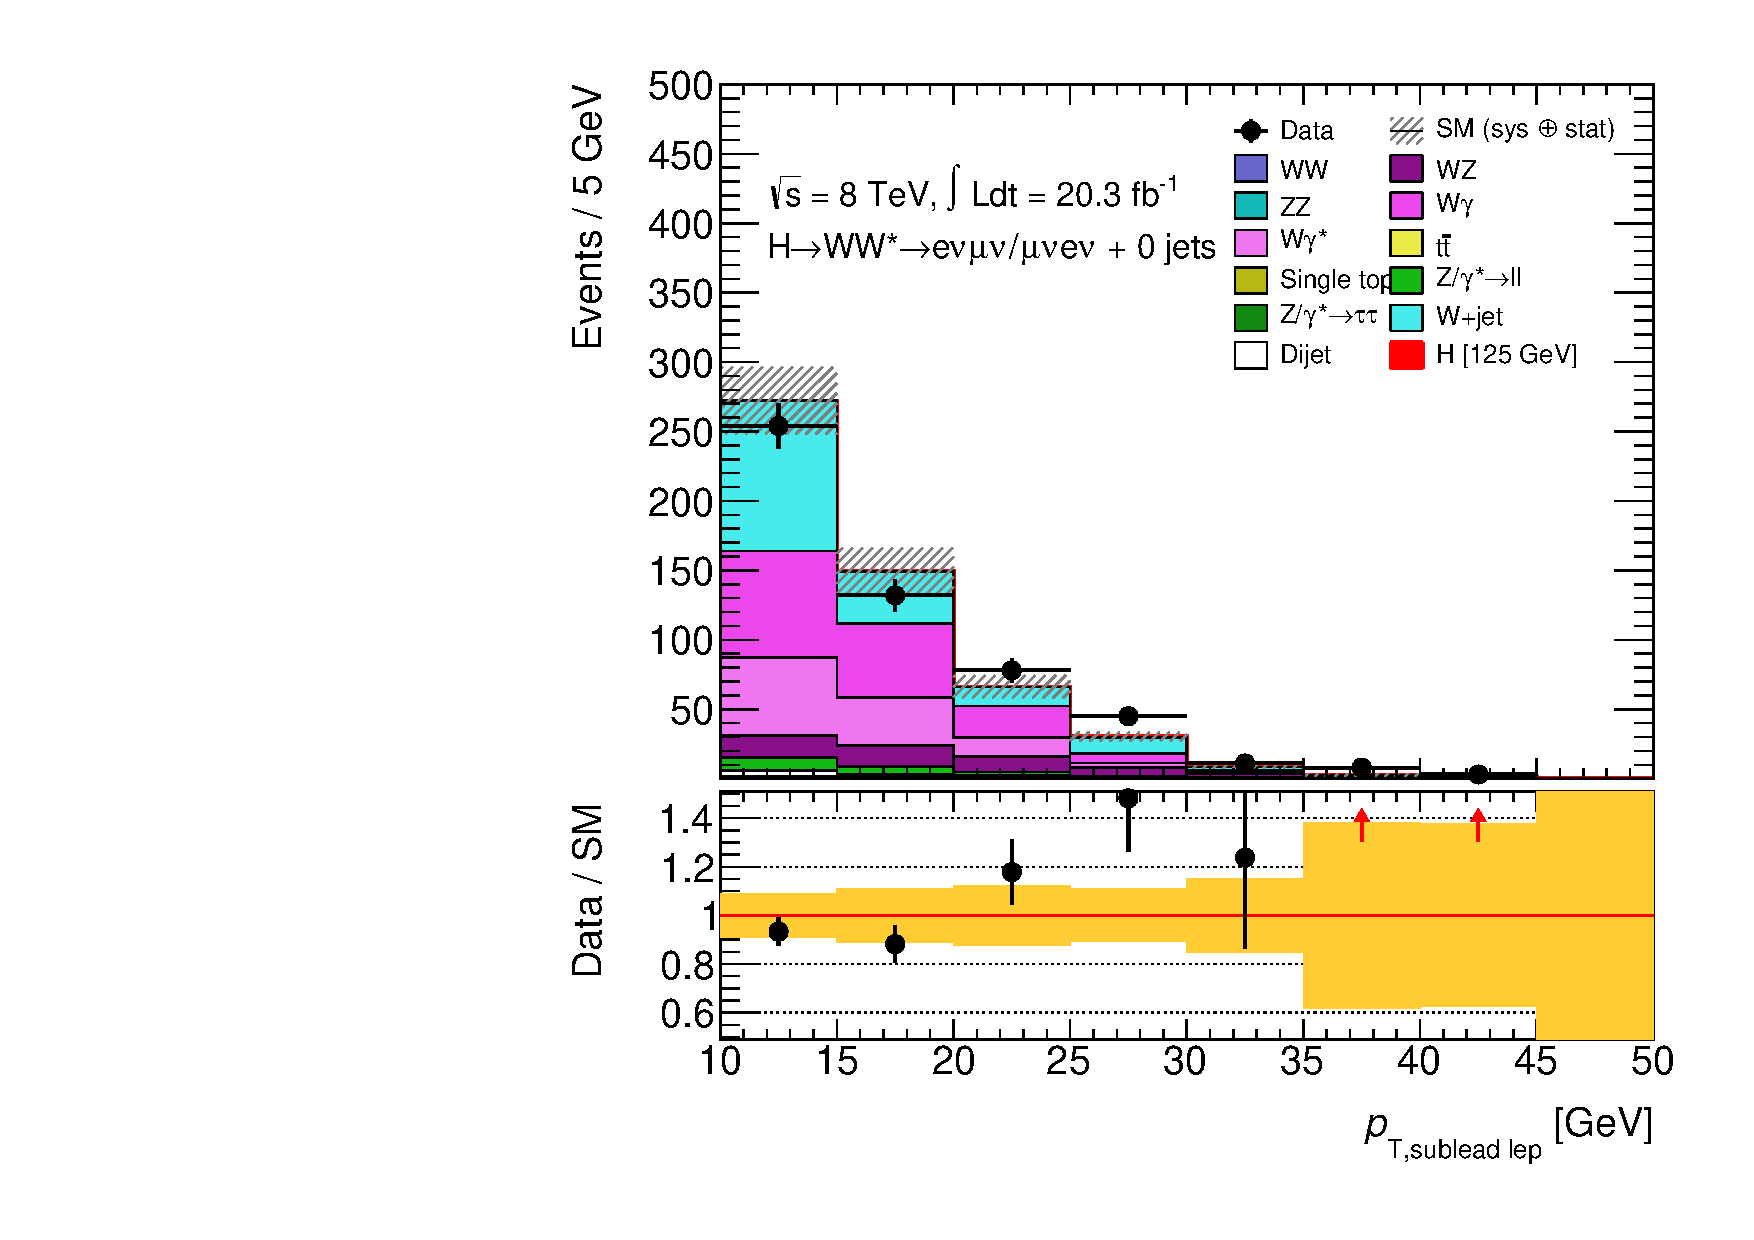
\includegraphics[width=0.48\textwidth]{tex/backgrounds/emme_CutFRecoil_0jet_sscr_lepPtSubLead_zoom_mh125_lin}
	\hfill
	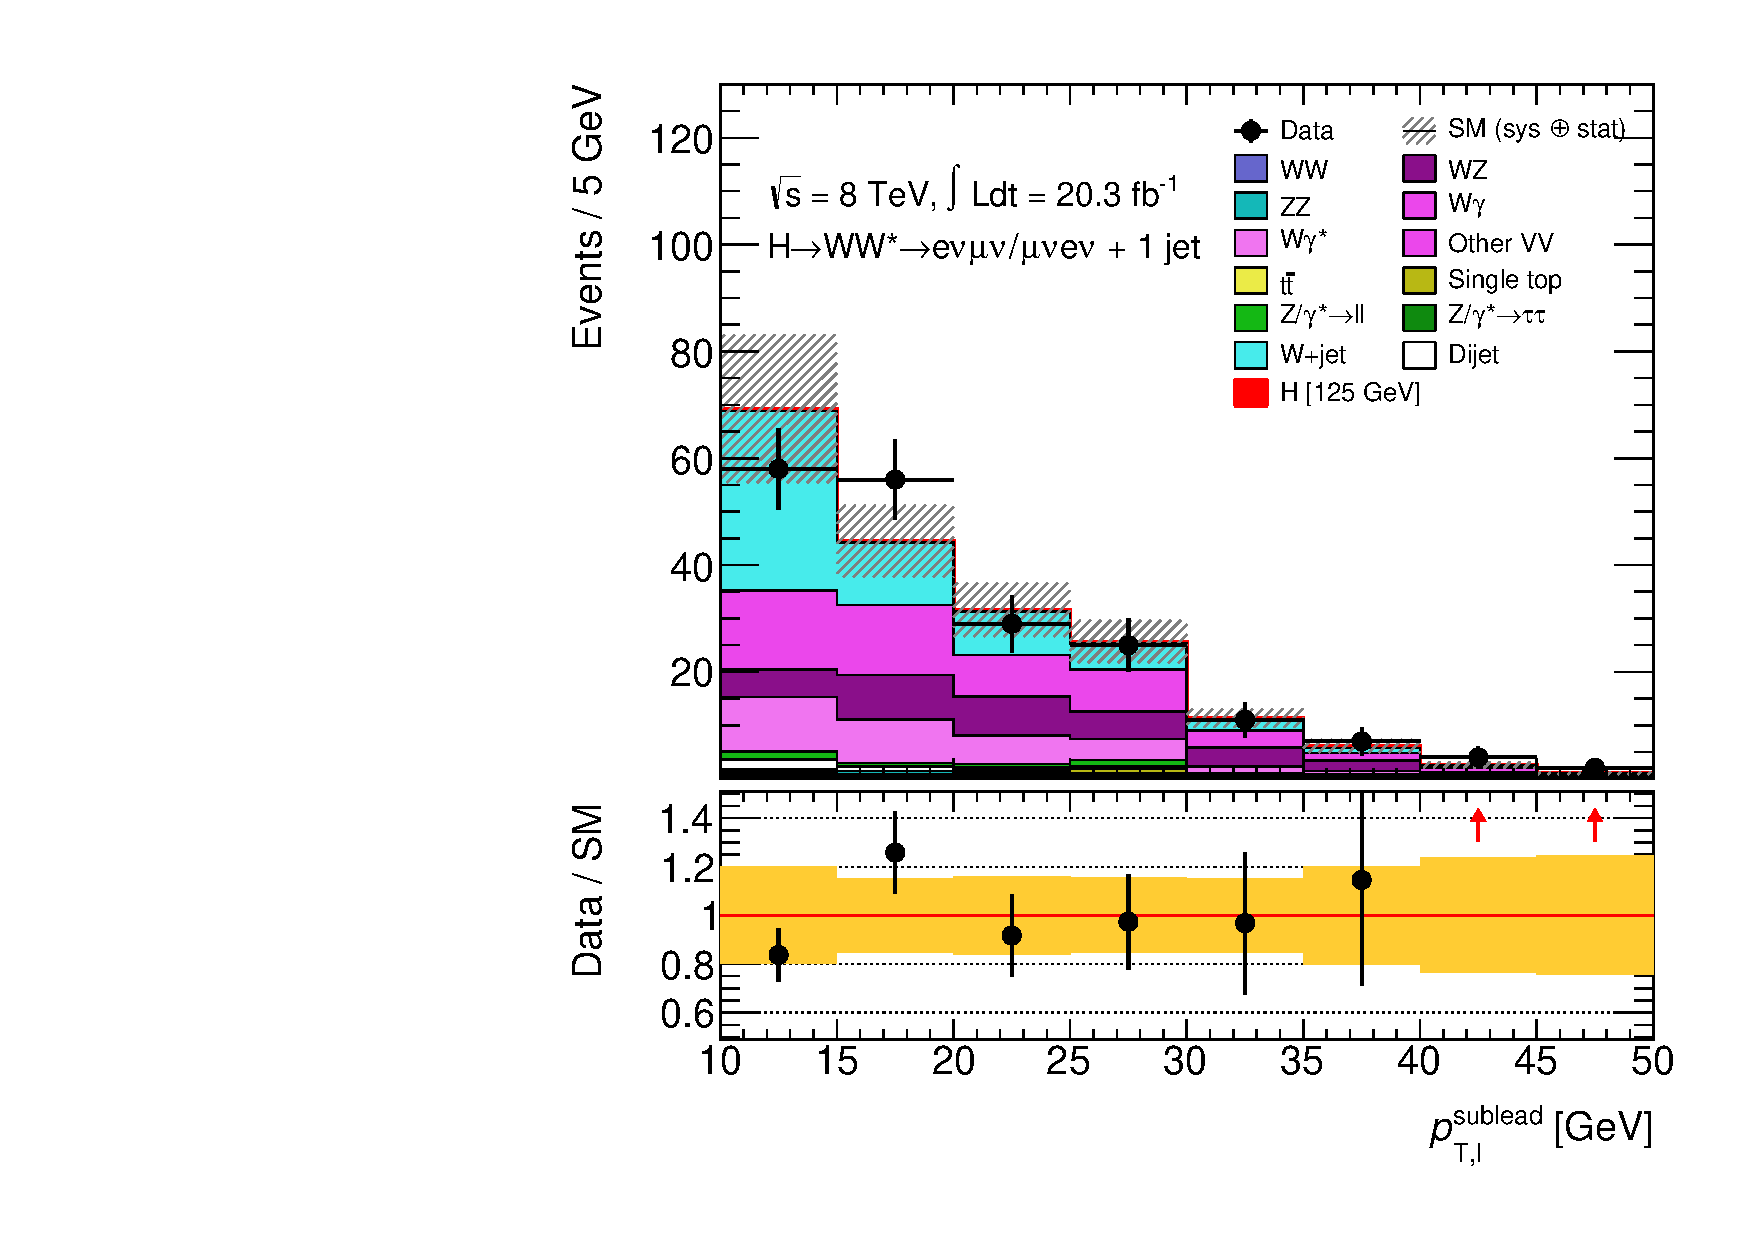
\includegraphics[width=0.48\textwidth]{tex/backgrounds/emme_CutFRecoil_1jet_sscr_lepPtSubLead_zoom_mh125_lin}
	\caption{The \mt (top), \mll (middle) and \ptsubleadlep (bottom) distributions in the 
	0-jet (left) and 1-jet (right) same-sign control regions. Normalisation factors are 
	applied.}
	\label{fig:sscr}
\end{figure}



\subsection{\Wgamma}
\label{sec:diboson:wgamma}

\Wgamma events enter the dilepton sample when the photon fakes an electron. This is usually 
caused by an asymmetric \HepProcess{\Pphoton \HepTo \epluseminus} conversion, where only 
one electron passes the object selection. This background is suppressed by the electron 
identification criteria, which require a hit in the first pixel layer and no conversion 
vertex (see \Section~\ref{sec:objects:electrons}).

\Wgamma is modelled by \meps{\alpgen}{\fherwig} and normalised to the NLO cross section 
calculated with \mcfm. Modelling is tested with a SS dilepton sample of \emch/\mech events, 
but where the electron object is required to have a conversion vertex and no hit in the 
first pixel layer (\ie the photon conversion rejection criteria are inverted). Validation 
regions (VRs) are defined in the 0-jet and 1-jet bins, using the corresponding signal 
region cuts. Experimental data are well described, as seen in \Figure~\ref{fig:wgamma:vr}.

\begin{figure}[t]
	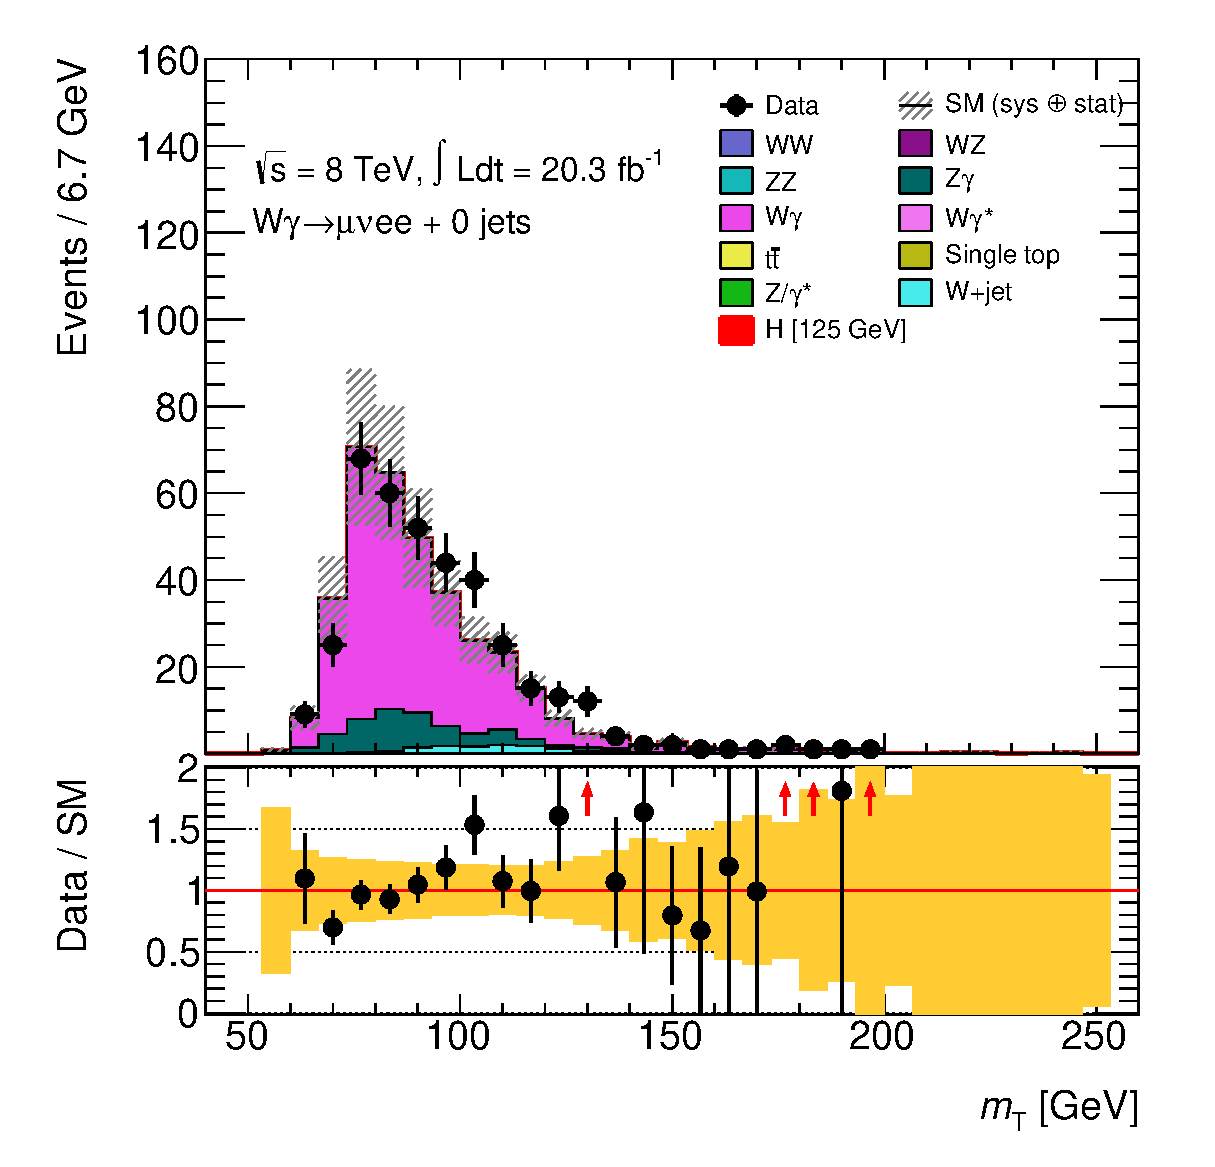
\includegraphics[width=0.48\textwidth]{tex/backgrounds/Wgamma/CutTopoDPhill_0jet_MT_TrackHWW_Clj_mh125_lin}
	\hfill
	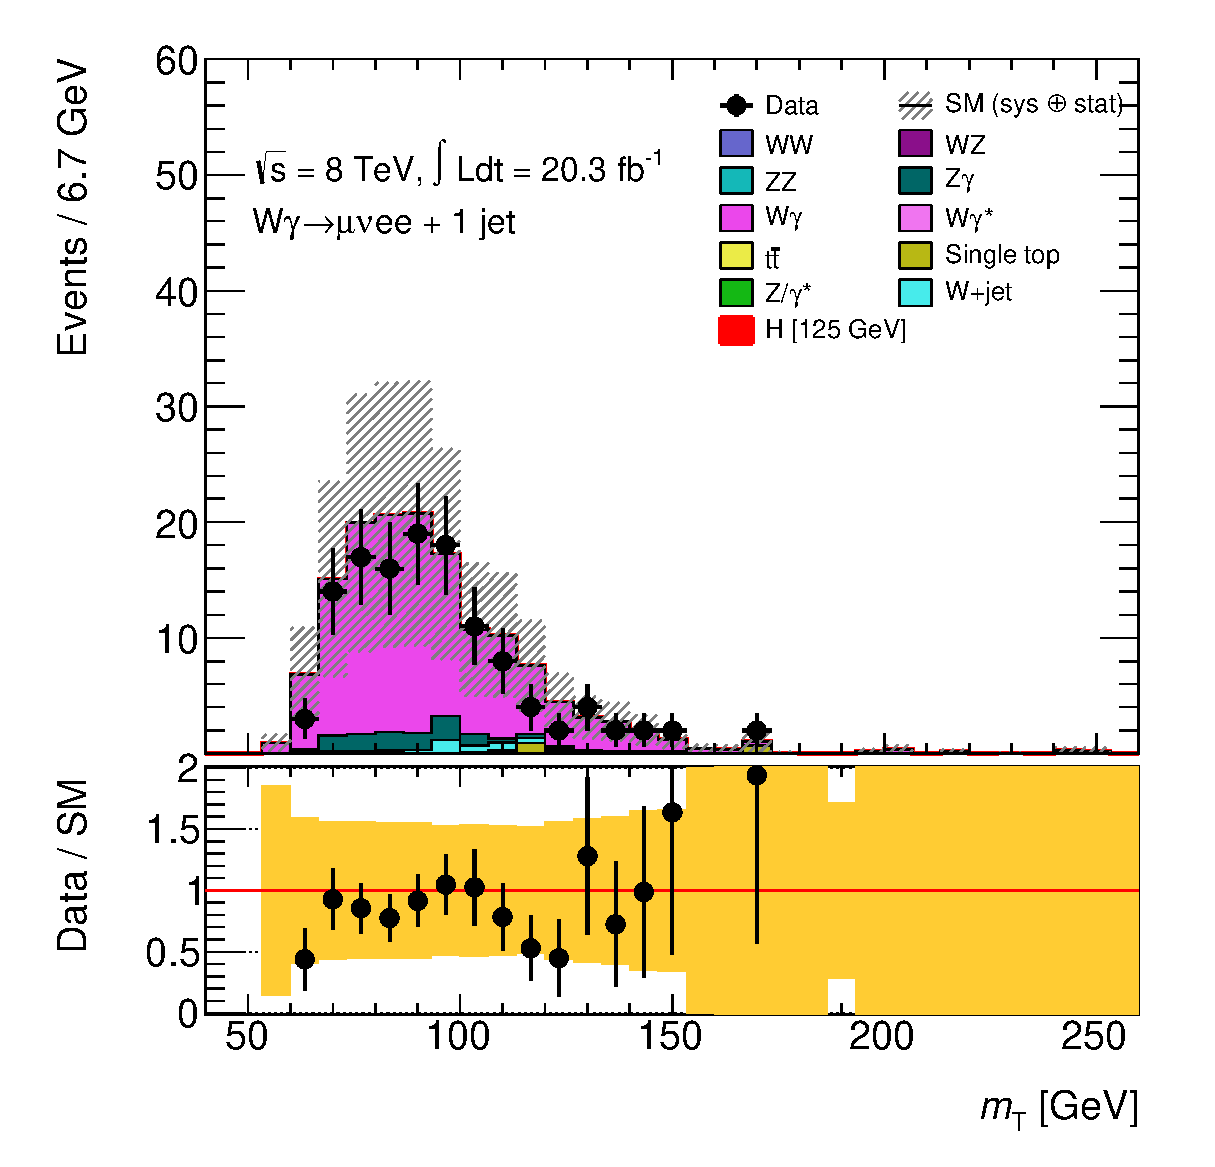
\includegraphics[width=0.48\textwidth]{tex/backgrounds/Wgamma/CutTopoDPhill_1jet_MT_TrackHWW_Clj_mh125_lin}
	\caption{The \mt distribution in the 0-jet (left) and 1-jet (right) \Wgamma validation 
	regions. The shaded error band includes statistical and theoretical uncertainties, in 
	addition to those associated with conversion modelling.}
	\label{fig:wgamma:vr}
\end{figure}

As the conversion and pixel hit criteria are inverted in the VR, their SR modelling is not 
tested in \Figure~\ref{fig:wgamma:vr}. Unfortunately, it is not possible to define a 
high-purity \Wgamma VR when including these criteria. Instead, 
a \HepProcess{\Zgamma \HepTo \Pmu\Pmu\Pphoton} VR is used to test this modelling. 
Events are selected with an OS muon pair with \unit{$p_{\text{T,\Pmu}}^{\text{lead}} > 
22$}{\GeV} and \unit{$p_{\text{T,\Pmu}}^{\text{sublead}} > 10$}{\GeV}, and an additional 
electron with \unit{$p_{\text{T,\Pe}} > 10$}{\GeV}. Low mass resonances are vetoed by 
\unit{$m_{\HepProcess{\Pmu\Pmu}} > 12$}{\GeV}, and events featuring QED FSR are selected by 
\unit{$\mods{m_{\HepProcess{\Pmu\Pmu\Pe}} - \mZ} < 15$}{\GeV}. The selected events are 
\about60\% \Zgamma and \about40\% \Zgstar. The mismodelling is found to depend upon 
$p_{\text{T,\Pe}}$ and so a conversion systematic uncertainty is derived: 25\% for 
\unit{10 -- 15}{\GeV}, 18\% for \unit{15 -- 20}{\GeV} and 5\% for \unit{$>\!20$}{\GeV}.



\subsection{\WZ and \Wgstar}
\label{sec:diboson:wgstar}

Both the \WZ and \Wgstar processes result in a \HepProcess{\Plepton\Pnu\Plepton'\Plepton'} 
final state, peaking in $m_{\HepProcess{\Plepton'\Plepton'}}$ at \mZ and 
$2m_{\Plepton'}$ respectively (due to the different \PZ and \Pphoton propagators). Their 
interference at intermediate $m_{\HepProcess{\Plepton'\Plepton'}}$ is non-negligible, and 
so these processes are generated together.

It is technically difficult to generate MC events with very low 
$m_{\HepProcess{\Plepton'\Plepton'}}$. For this reason, the phase space is generated in two 
parts: high mass ``\WZ'' events with \unit{$m_{\HepProcess{\Plepton'\Plepton'}} > 7$}{\GeV} 
and low mass ``\Wgstar'' events with 
\unit{$m_{\HepProcess{\Plepton'\Plepton'}} < 7$}{\GeV}.\footnote{
	It is these ``\WZ'' and ``\Wgstar''	MC samples that are referred to as the \WZ and 
	\Wgstar backgrounds, though each sample contains both the \WZ and \Wgstar processes.
}
In ambiguous cases ($\Plepton = \Plepton'$), the lowest mass opposite-sign same-flavour 
dilepton pair is used to split the phase space. \WZ is modelled at NLO by 
\meps{\powhegbox}{\pythia{8}}.

\Wgstar is technically difficult to model because it involves integrating over a phase 
space with extremely low mass; the threshold for production is 
$m_{\HepProcess{\Plepton'\Plepton'}} = 2m_{\Plepton'}$, which is \unit{1.022}{\MeV} for 
\HepProcess{\Plepton\Pnu\Pe\Pe}. In previous analysis iterations, \Wgstar was modelled by 
\meps{\madgraph}{\pythia{6}} \cite{HWW-Moriond}. However, this implementation failed to 
produce gauge-invariant results when $m_{\HepProcess{\Plepton'\Plepton'}} \ll \Gamma_{\PW}$ 
\cite{MadGraph:Wgstar}, yielding wildly unphysical events in this region of phase space 
(\eg leptons with \unit{\pt~\about~1}{\TeV}). In an attempt to resolve this problem, events 
with \unit{$m_{\HepProcess{\Plepton'\Plepton'}} < 3$}{\MeV} were removed from the MC 
sample, and events with \unit{3}{\MeV} $< m_{\HepProcess{\Plepton'\Plepton'}} <$ 
\unit{10}{\MeV} were reweighted in order to recover the cross section. Even with this fix, 
this background was associated with a modelling uncertainty of 40\% (evaluated by comparing 
to \sherpa).

\sherpa can produce gauge-invariant results for the full mass range, since it employs a 
complex mass scheme \cite{Sherpa:Wgstar}. A simple LO \sherpa sample underestimates the FSR 
phase space with $p_{\text{T,\HepProcess{\Plepton'\Plepton'}}} > \mW/2$. For this reason, 
\Wgstar is modelled by ME-PS merging with up to one additional parton (see 
\Section~\ref{sec:mc:merging}). It is technically not possible to include further partons 
in the ME-PS merging over the full mass range.

The \sherpa sample is normalised using an NLO $K$-factor of $0.94\pm0.07\,\text{(scale)}$, 
calculated with \mcfm. Due to technical limitations, this is calculated in a high mass 
region \unit{$m_{\HepProcess{\Plepton'\Plepton'}} \in \hardrange{0.5,7}$}{\GeV} and then 
extrapolated down in mass. It is calculated with the \unit{$\ptleadlep > 22$}{\GeV} and 
\unit{$\ptsubleadlep > 10$}{\GeV} criteria.

Since the \Wgstar acceptance of the lepton \pt criteria is strongly related to \njets and 
because the \HWW analysis itself is jet binned, the jet multiplicity distribution must be 
well modelled. For this reason, the \njets distribution is reweighted to that of a \sherpa 
ME-PS merged sample with up to two additional partons, using corrections of 
$0.91\pm0.06\,\text{(scale)}$ in the 0-jet bin, $1.09\pm0.33\,\text{(scale)}$ in the 1-jet 
bin, and $2.0\pm0.5\,\text{(scale)}$ in the \twojet bin. Again, due to technical 
limitations, this was calculated in a high mass region 
\unit{$m_{\HepProcess{\Plepton'\Plepton'}} \in \hardrange{0.5,7}$}{\GeV} and then 
extrapolated down in mass. It was also calculated following the 
\unit{$\ptleadlep > 22$}{\GeV} and \unit{$\ptsubleadlep > 10$}{\GeV} criteria.

Two sources of theoretical uncertainties in the signal region acceptances are considered: 
higher order corrections are estimated by varying \mur and \muf as described elsewhere in 
this thesis, and modelling uncertainties are evaluated by comparing the \sherpa ME-PS 
samples with $\leq\!1$ and $\leq\!2$ partons in a high mass region 
\unit{$m_{\HepProcess{\Plepton'\Plepton'}} \in \hardrange{0.5,7}$}{\GeV}. These are 
negligible compared to the theoretical uncertainties in the $K$-factor and jet bin 
correction. Scale uncertainties in the shape of the \mt distribution are also evaluated.

The \Wgstar modelling is tested in a \HepProcess{\Wgstar \HepTo \Pe\Pnu\Pmu\Pmu} validation 
region (VR). Since $\Delta R\parenths{\Pmu,\Pmu}$ is generally small, the muon isolation 
criteria are altered: tracks associated with other muons are removed from the 
$p_{\text{T}}^{\text{cone}}$ definition, and the calorimeter isolation is loosened to 
$\etcone{0.3}/\pt < 0.4$ for \unit{$\pt < 15$}{\GeV} (\cf \Section~\ref{sec:objects:muons}).
Events are selected with \unit{$p_{\text{T,\Pe}} > 22$}{\GeV}, 
\unit{$p_{\text{T,\Pmu}}^{\text{lead}} > 10$}{\GeV} and 
\unit{$p_{\text{T,\Pmu}}^{\text{sublead}} > 3$}{\GeV}. 
Then, the VR is defined by \unit{$m_{\HepProcess{\Pmu\Pmu}} < 7$}{\GeV}, 
\unit{$\mods{m_{\HepProcess{\Pmu\Pmu}} - m_{\PJpsi}} > 100$}{\MeV}, 
\unit{$\metrel > 20$}{\GeV} and $\max\parenths{\dphill} < 2.8$.
The experimental data in the VR is well described by \sherpa, as seen in 
\Figure~\ref{fig:wgstar:vr}, and supports the normalisation used. It appears that \njets is 
underestimated, though this effect is within theoretical uncertainties (which are not shown 
in \Figure~\ref{fig:wgstar:vr}).

\begin{figure}[t]
	\includegraphics[width=0.48\textwidth]{tex/backgrounds/Wgstar/em_CutDPhiMax_lepPtSublead_zoom_mh125_lin}
	\hfill
	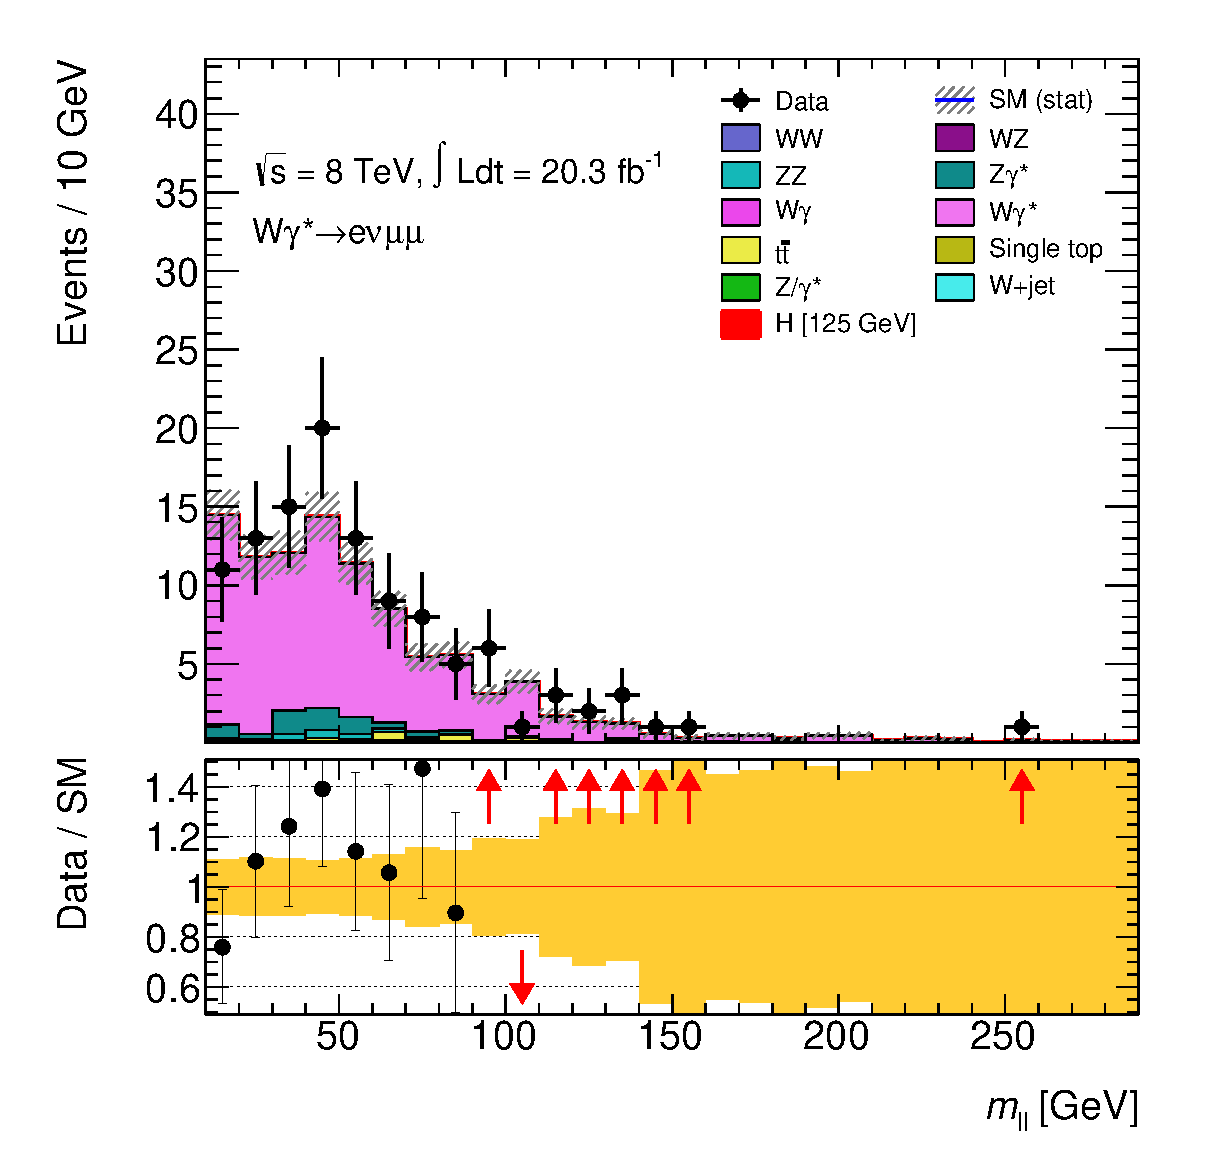
\includegraphics[width=0.48\textwidth]{tex/backgrounds/Wgstar/em_CutDPhiMax_Mll_mh125_lin}
	\\
	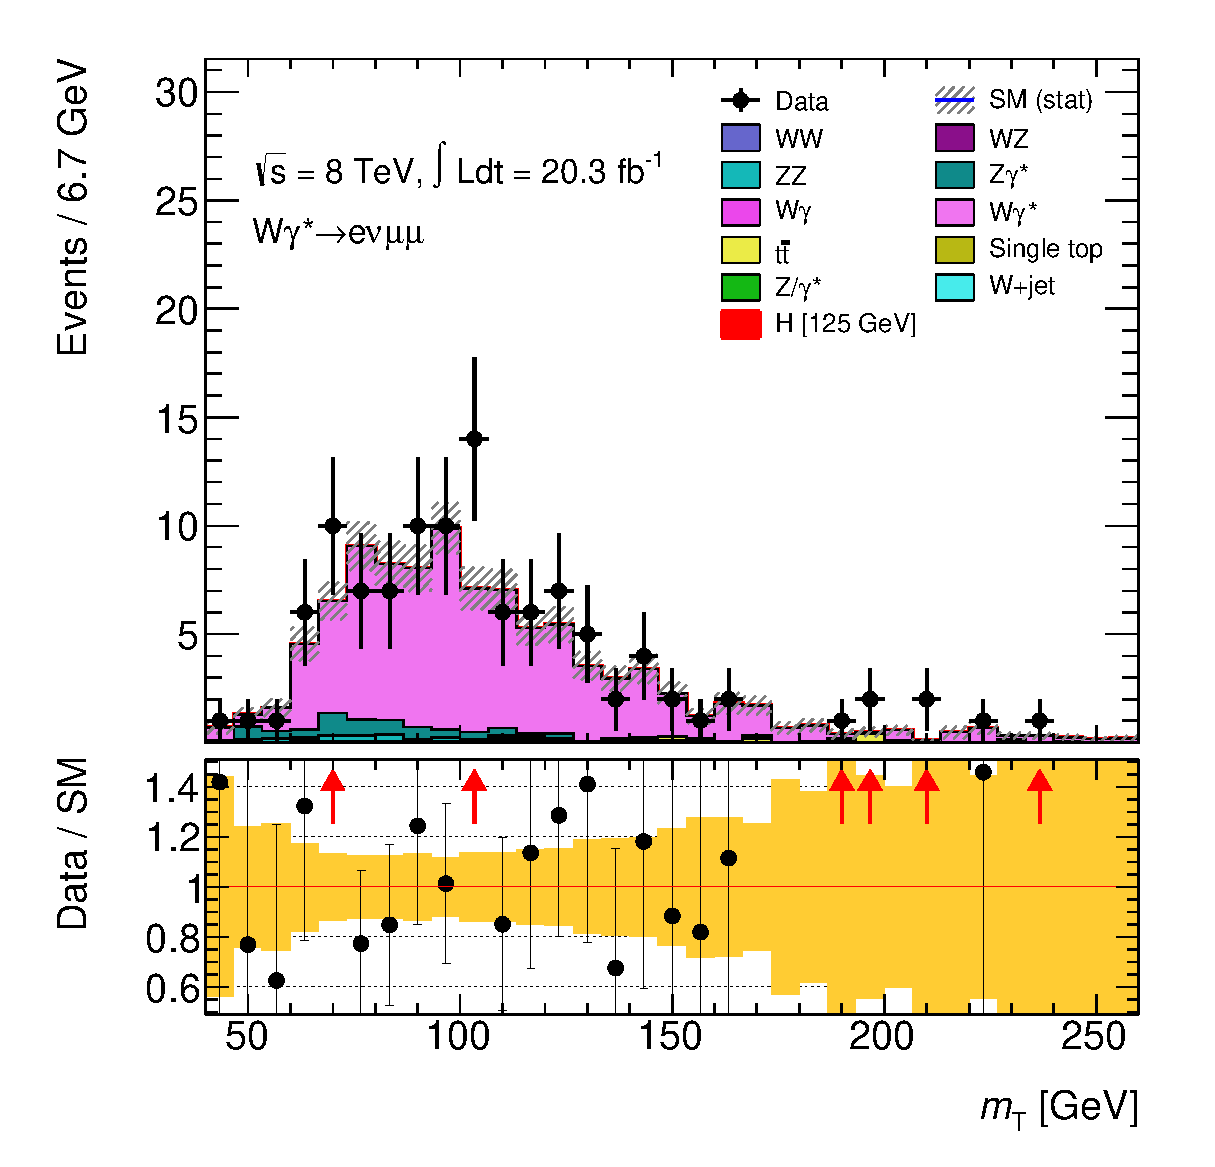
\includegraphics[width=0.48\textwidth]{tex/backgrounds/Wgstar/em_CutDPhiMax_MT_TrackHWW_Clj_mh125_lin}
	\hfill
	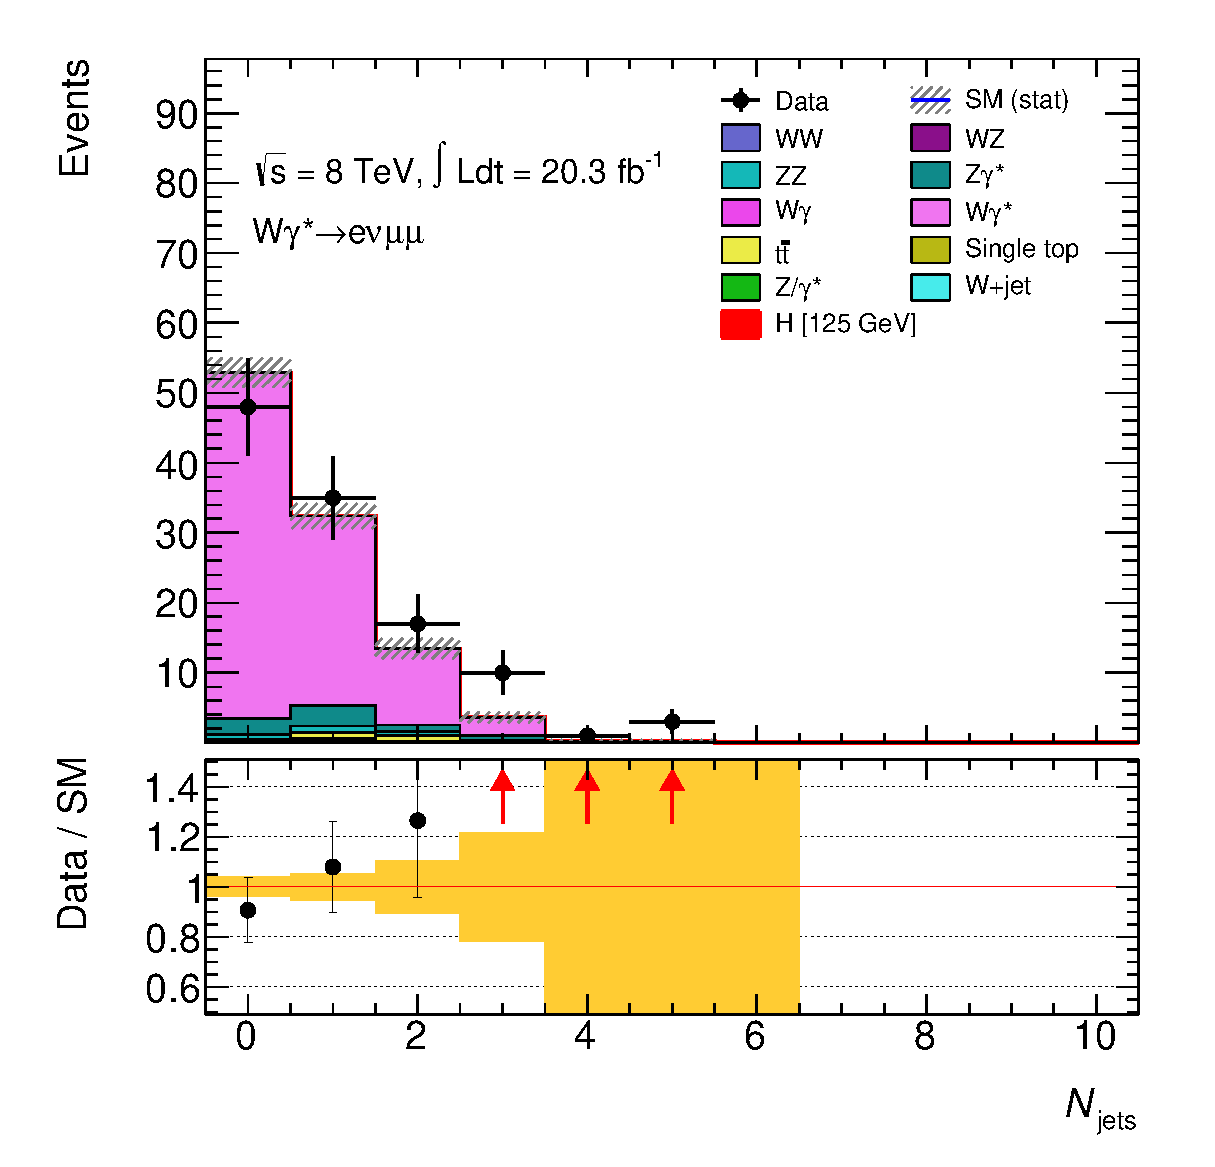
\includegraphics[width=0.48\textwidth]{tex/backgrounds/Wgstar/em_CutDPhiMax_m_jet_n_mh125_lin}
	\caption{The \ptsubleadlep (top left), \mll (top right), \mt (bottom left) and \njets 
	(bottom right) distributions in the \Wgstar validation region. Leptonic observables are 
	defined with the electron and the leading muon.}
	\label{fig:wgstar:vr}
\end{figure}

It should be noted that the \Wgstar VR does not test the modelling of 
\HepProcess{\Wgstar \HepTo \Plepton\Pnu\Pe\Pe}, which can contribute background events via 
an additional mechanism: both electrons can be reconstructed as a single electron when 
$\Delta R\parenths{\Pe,\Pe}$ is very small. However, the good agreement in the same-sign 
control region suggests that this is well modelled.



\subsection{\ZZ and \Zgstar}
\label{sec:diboson:zz}

Similar to \Section~\ref{sec:diboson:wgstar}, the \ZZ and \Zgstar processes share a 
\HepProcess{\Plepton\Plepton\Plepton'\Plepton'} final state, and are modelled together in 
order to include their interference. Again, the phase space is split: high mass 
``\ZZ'' events with \unit{$m_{\HepProcess{\Plepton\Plepton}} > 4$}{\GeV} and 
\unit{$m_{\HepProcess{\Plepton'\Plepton'}} > 4$}{\GeV}, and low mass ``\Zgstar'' events 
with \unit{$m_{\HepProcess{\Plepton\Plepton}} > 4$}{\GeV} and 
\unit{$m_{\HepProcess{\Plepton'\Plepton'}} < 4$}{\GeV}.\footnote{
	It is these ``\ZZ'' and ``\Zgstar''	MC samples that are referred to as the \ZZ and 
	\Zgstar backgrounds, though each sample contains both the \ZZ and \Zgstar processes.
}
The corresponding ``\HepProcess{\Pgammastar\Pgammastar}'' process is not modelled due to 
technical limitations. In ambiguous cases ($\Plepton = \Plepton'$), the lowest mass 
opposite-sign same-flavour dilepton pair is used to split the phase space.

\ZZ is modelled at NLO by \meps{\powhegbox}{\pythia{8}} and the NNLO \ggZZ diagrams are 
also modelled by \meps{\ggtozz}{\fherwig}. \Zgstar is modelled by \sherpa and is normalised 
to the NLO cross section calculated with \mcfm. As in \Section~\ref{sec:diboson:wgstar}, 
this $K$-factor is calculated at high $m_{\HepProcess{\Plepton'\Plepton'}}$ and 
extrapolated to low $m_{\HepProcess{\Plepton'\Plepton'}}$.

Neither background contributes significantly to the signal region. However, it is important 
to model the \Zgstar background in the \Zgamma validation region (see 
\Section~\ref{sec:diboson:wgamma}) and when measuring the \Zjets fake factor (see 
\Section~\ref{sec:wjets:zjet_ff}).


\section{Top}
	\label{sec:top}
	%!TEX root = ../../thesis.tex

The leading and subleading contributions to the top background are the \ttbar and 
\HepProcess{\PW\Ptop} processes, respectively. These are irreducible backgrounds, in that 
they both exhibit the opposite-sign dilepton + \met experimental signature. This occurs via 
top decays $\text{BR}\parenths{\HepProcess{\Ptop \HepTo \PW\Pbottom}} \approx 100\%$ 
(occurs before hadronisation) and leptonic \PW boson decays.

Considering \HepProcess{\ttbar \HepTo \PW\PW\Pbottom\Pbottom} and \HepProcess{\PW\Ptop 
\HepTo \PW\PW\Pbottom}, it is clear that top events feature one or two \Pbottom-jets. This 
motivates the jet binning of the \HWW analysis (see \Figure~\ref{fig:sel:njets}), using 
jets with a \pt threshold of \unit{25(30)}{\GeV} in the central (forward) region (see 
\Section~\ref{sec:objects:jets}). The top background is further discriminated by counting 
the number of \Pbottom-tagged jets with \unit{$\pt > 20$}{\GeV} in the central region, 
using an algorithm with a tagging efficiency of 85\% (see \Section~\ref{sec:objects:bjets}).
In the 1-jet and \twojet bins, the top background is suppressed by vetoing events with 
\Pbottom-tagged jets.

\ttbar, \HepProcess{\PW\Ptop} and $s$-channel single top are modelled by 
\meps{\powhegbox}{\pythia{6}}, while $t$-channel single top is modelled by 
\meps{\acermc}{\pythia{6}}. However, the jet binning and \Pbottom-tagged jet veto 
introduce large modelling uncertainties, and so data-driven techniques are used to 
estimate this background.



\subsection{0-jet bin estimation}
\label{sec:top:0j}

In the 0-jet bin, the top background is very small because both \Pbottom-jets must fail the 
jet selection. It is estimated by the data-driven \textit{jet veto survival probability 
method} since the jet veto efficiency $\epsilon_0$ has large uncertainties.

An extended signal region (ESR) is defined by the pre-selection in 
\Section~\ref{sec:selection:presel}, with an additional $\dphill < 2.8$ criterion to 
suppress the \DYtt background. The aim is to estimate the number of events in the ESR 
passing the jet veto $N_{\text{top}}^{\text{pred,ESR,0j}}$, and then extrapolate to the 
0-jet signal region (SR) with MC
\begin{equation}
	N_{\text{top}}^{\text{pred,SR,0j}} &= \alpha_{\text{top}}^{\text{0j}} \cdot \epsilon_{\text{0,top}}^{\text{pred,ESR}} \cdot \parenths{N^{\text{data,ESR}} - N_{\text{non-top}}^{\text{pred,ESR}}} \\
	\alpha_{\text{top}}^{\text{0j}} &= N_{\text{top}}^{\text{MC,SR,0j}} / N_{\text{top}}^{\text{MC,ESR,0j}}
\end{equation}
where $\epsilon_{0}$ is the jet veto efficiency. \Figure~\ref{fig:sel:njets} shows that, 
after pre-selection, top dominates the \emch/\mech channels, but \DYll dominates the 
\eech/\mmch channels. For this reason, the top normalisation is derived from a combined 
\emch{}+\mech channel and extrapolated to each \emch/\mech/\eech/\mmch SR.

The ESR is dominated by \ttbar events featuring two \Pbottom-jets. Since each 
\Pbottom-quark originates from the decay of a top quark, the kinematic distributions of the 
two jets are similar. Thus, it is possible to make the approximation 
$\epsilon_{\text{0,top}} = \epsilon_{\text{1,top}}^2$, where $\epsilon_{1}$ is the veto 
efficiency of a second jet. This $\epsilon_{\text{1,top}}$ is experimentally measured in a 
high-purity top control region (CR) and is used to correct the $\epsilon_{\text{0,top}}$ 
modelled by MC in the ESR:
\begin{equation}
	\epsilon_{\text{0,top}}^{\text{pred,ESR}} &= \epsilon_{\text{0,top}}^{\text{MC,ESR}} \parenths{\frac{\epsilon_{1}^{\text{data,CR}}}{\epsilon_{\text{1,top}}^{\text{MC,CR}}}}^{\!\!2} \,. \label{eq:jvsp}
\end{equation}
The top CR requires at least one \Pbottom-tagged jet with \unit{$\pt > 25$}{\GeV}, relative 
to the ESR. Then $\epsilon_{\text{1,top}}^{\text{data,CR}}$ is measured by counting the 
fraction of CR events with zero additional jets. These are defined as jets with 
$\Delta R > 1$ from the highest scoring \Pbottom-tagged jet (see \Figure~\ref{fig:top:jvsp}).
It is found that (\ref{eq:jvsp}) is not invalidated by contributions from other top 
processes and jets other than the two \Pbottom-jets.

\begin{figure}[t]
	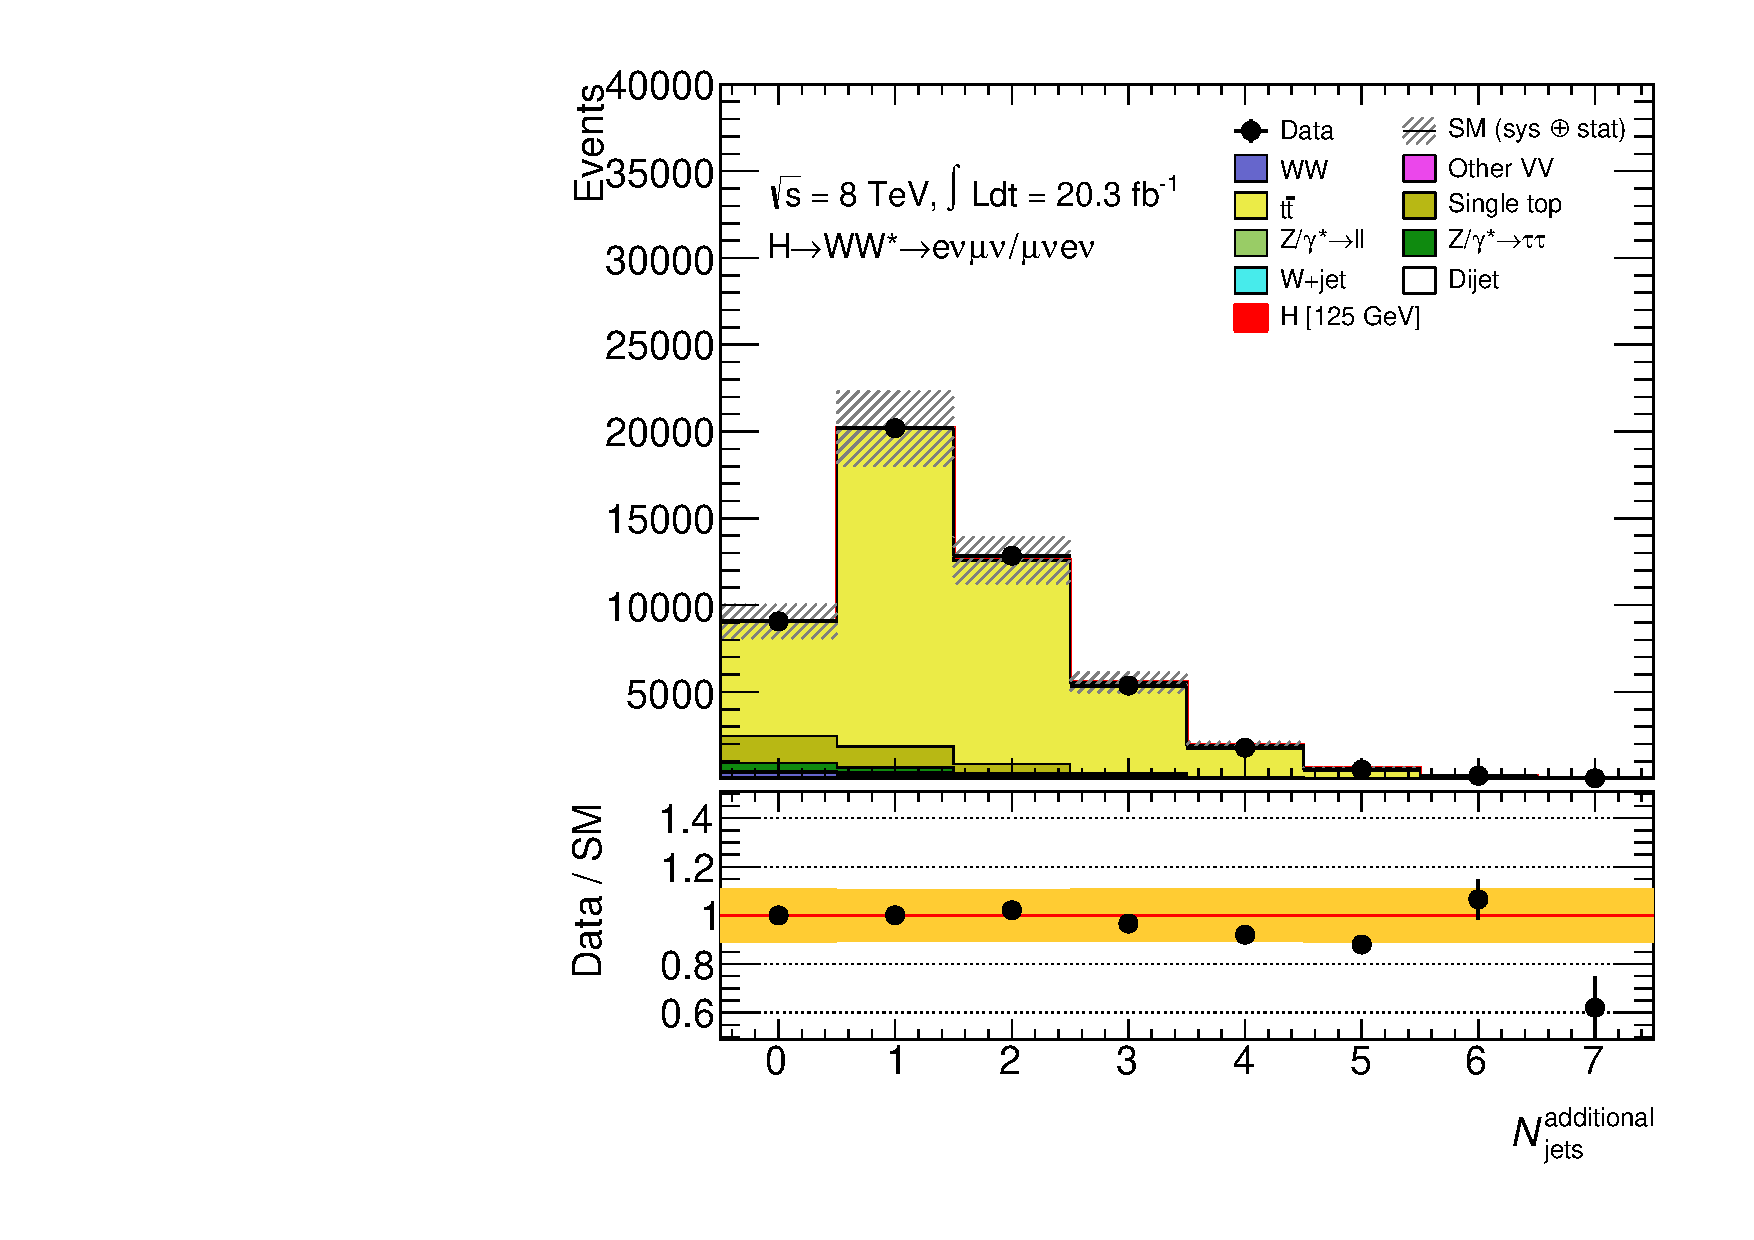
\includegraphics[width=0.495\textwidth]{tex/backgrounds/emme_CutTopControl_AddTrackMET_nJets_probing_mh125_lin}
	\hfill
	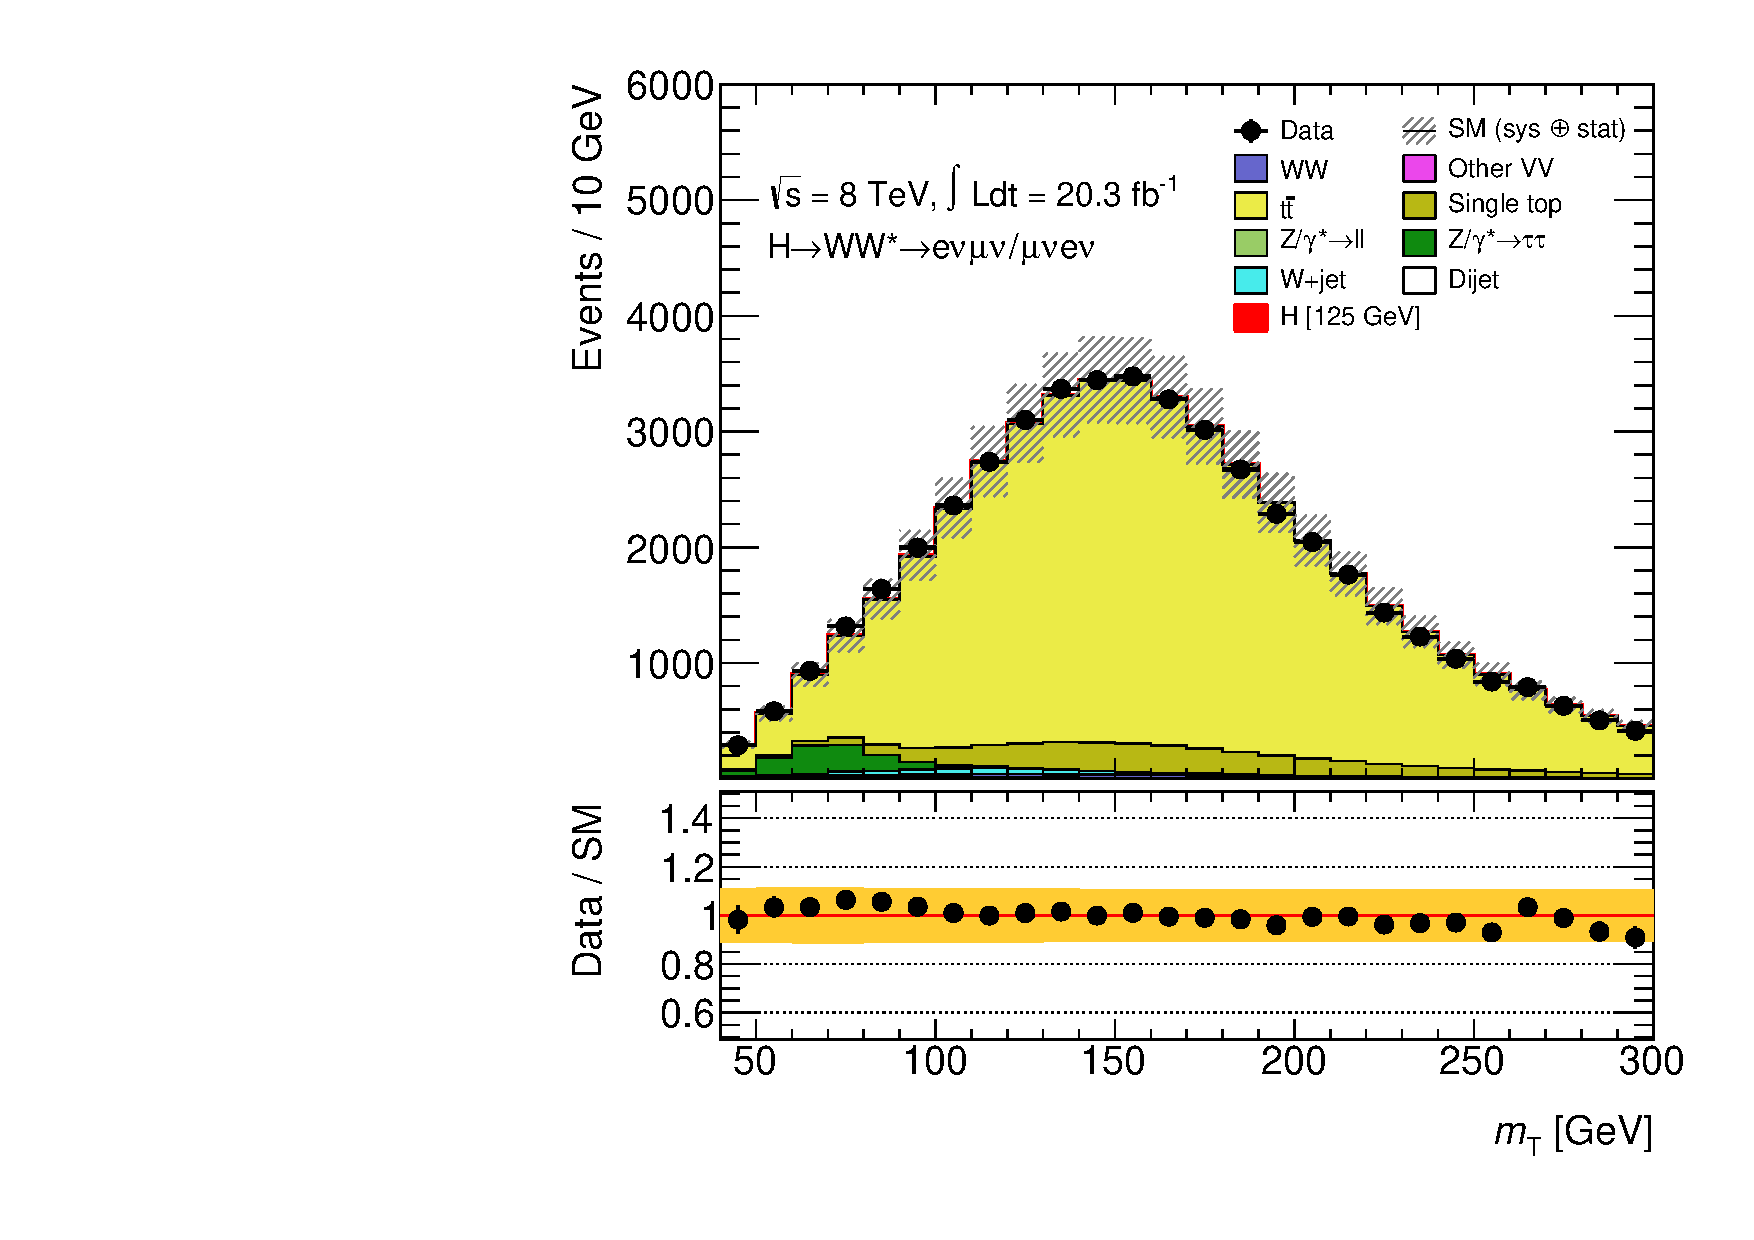
\includegraphics[width=0.495\textwidth]{tex/backgrounds/emme_CutTopControl_AddTrackMET_MT_TrackHWW_Clj_mh125_lin}
	\caption{The number of additional jets (left) and the \mt distribution (right) in the 
	top control region used by the jet veto survival probability method. The fraction of 
	events with zero additional jets is $\epsilon_{\text{1,top}}^{\text{data,CR}}$, as 
	described in the text.}
	\label{fig:top:jvsp}
\end{figure}

The total uncertainties in the expected 0-jet top background is \about8.2\%, dominated by 
theoretical uncertainties in the extrapolation $\alpha_{\text{top}}^{\text{0j}}$ and 
JES/JER uncertainties in the predicted jet veto efficiency 
$\epsilon_{\text{0,top}}^{\text{pred,ESR}}$.

To estimate the top background in 0-jet regions other than the SR, the method is viewed as 
providing a simple data-driven normalisation factor. This is equivalent to neglecting the 
extrapolation uncertainties, but is helpful when plotting observables. The normalisation 
factor is measured to be \stat{1.115}{0.031}\todo{update}.



\subsection{1-jet bin estimation}
\label{sec:top:1j}

In the 1-jet bin, the top background is suppressed by removing events with a 
\Pbottom-tagged jet with \unit{$\pt > 20$}{\GeV}. Since the \Pbottom-tagging efficiency is 
associated with large uncertainties, the data-driven \textit{jet \Pbottom-tagging 
efficiency extrapolation method} is used to estimate this background.

An extended signal region (ESR) is defined by the pre-selection in 
\Section~\ref{sec:selection:presel}. Since it is the $\njets = 1$ selection and the 
\Pbottom-tagged jet veto that introduce the largest uncertainties to this background, the 
aim of the method is to estimate the number of events accepted by these cuts 
$N_{\text{top}}^{\text{pred,ESR,1j0\Pbottom}}$, and then extrapolate to the 1-jet signal 
region (SR) with MC
\begin{equation}
	N_{\text{top}}^{\text{pred,SR,1j0\Pbottom}} &= \alpha_{\text{top}}^{\text{1j}} \cdot N_{\text{top}}^{\text{pred,ESR,1j0\Pbottom}} \\
	\alpha_{\text{top}}^{\text{1j}} &= N_{\text{top}}^{\text{MC,SR,1j0\Pbottom}} / N_{\text{top}}^{\text{MC,ESR,1j0\Pbottom}} \,.
\end{equation}
The top normalisation is derived from a combined \emch{}+\mech channel and extrapolated to 
each \emch/\mech/\eech/\mmch SR.

In order to estimate $N_{\text{top}}^{\text{pred,ESR,1j0\Pbottom}}$, the number of 1-jet 
events in the ESR with a \Pbottom-tagged jet $N^{\text{data,ESR,1j1\Pbottom}}$ is measured, 
which is highly pure in top events (see \Figure~\ref{fig:top:jbee})\todo{Add systematics to 
error band}. Then the non-top contamination is subtracted, and the \Pbottom-tagged jet 
selection is inverted using the expected \Pbottom-tagging efficiency 
$\varepsilon_{\Pbottom}^{\text{pred,ESR,1j}}$:
\begin{equation}
	N_{\text{top}}^{\text{pred,SR,1j0\Pbottom}} &= \alpha_{\text{top}}^{\text{1j}} \cdot \frac{1 - \varepsilon_{\Pbottom}^{\text{pred,ESR,1j}}}{\varepsilon_{\Pbottom}^{\text{pred,ESR,1j}}} \cdot \parenths{N^{\text{data,ESR,1j1\Pbottom}} - N_{\text{non-top}}^{\text{pred,ESR,1j1\Pbottom}}} \,.
\end{equation}
It should be emphasised that $\varepsilon_{\Pbottom}$ is a per-jet efficiency, rather than 
a per-event efficiency (\cf $\epsilon_0$). Also, $\varepsilon_{\Pbottom}$ is the average 
\Pbottom-tagging efficiency for a jet in a top event, and will include non-\Pbottom-jets 
(\ie it is a mixture of tagged \Pbottom-jets and mis-tagged other jets).

\begin{figure}[t]
	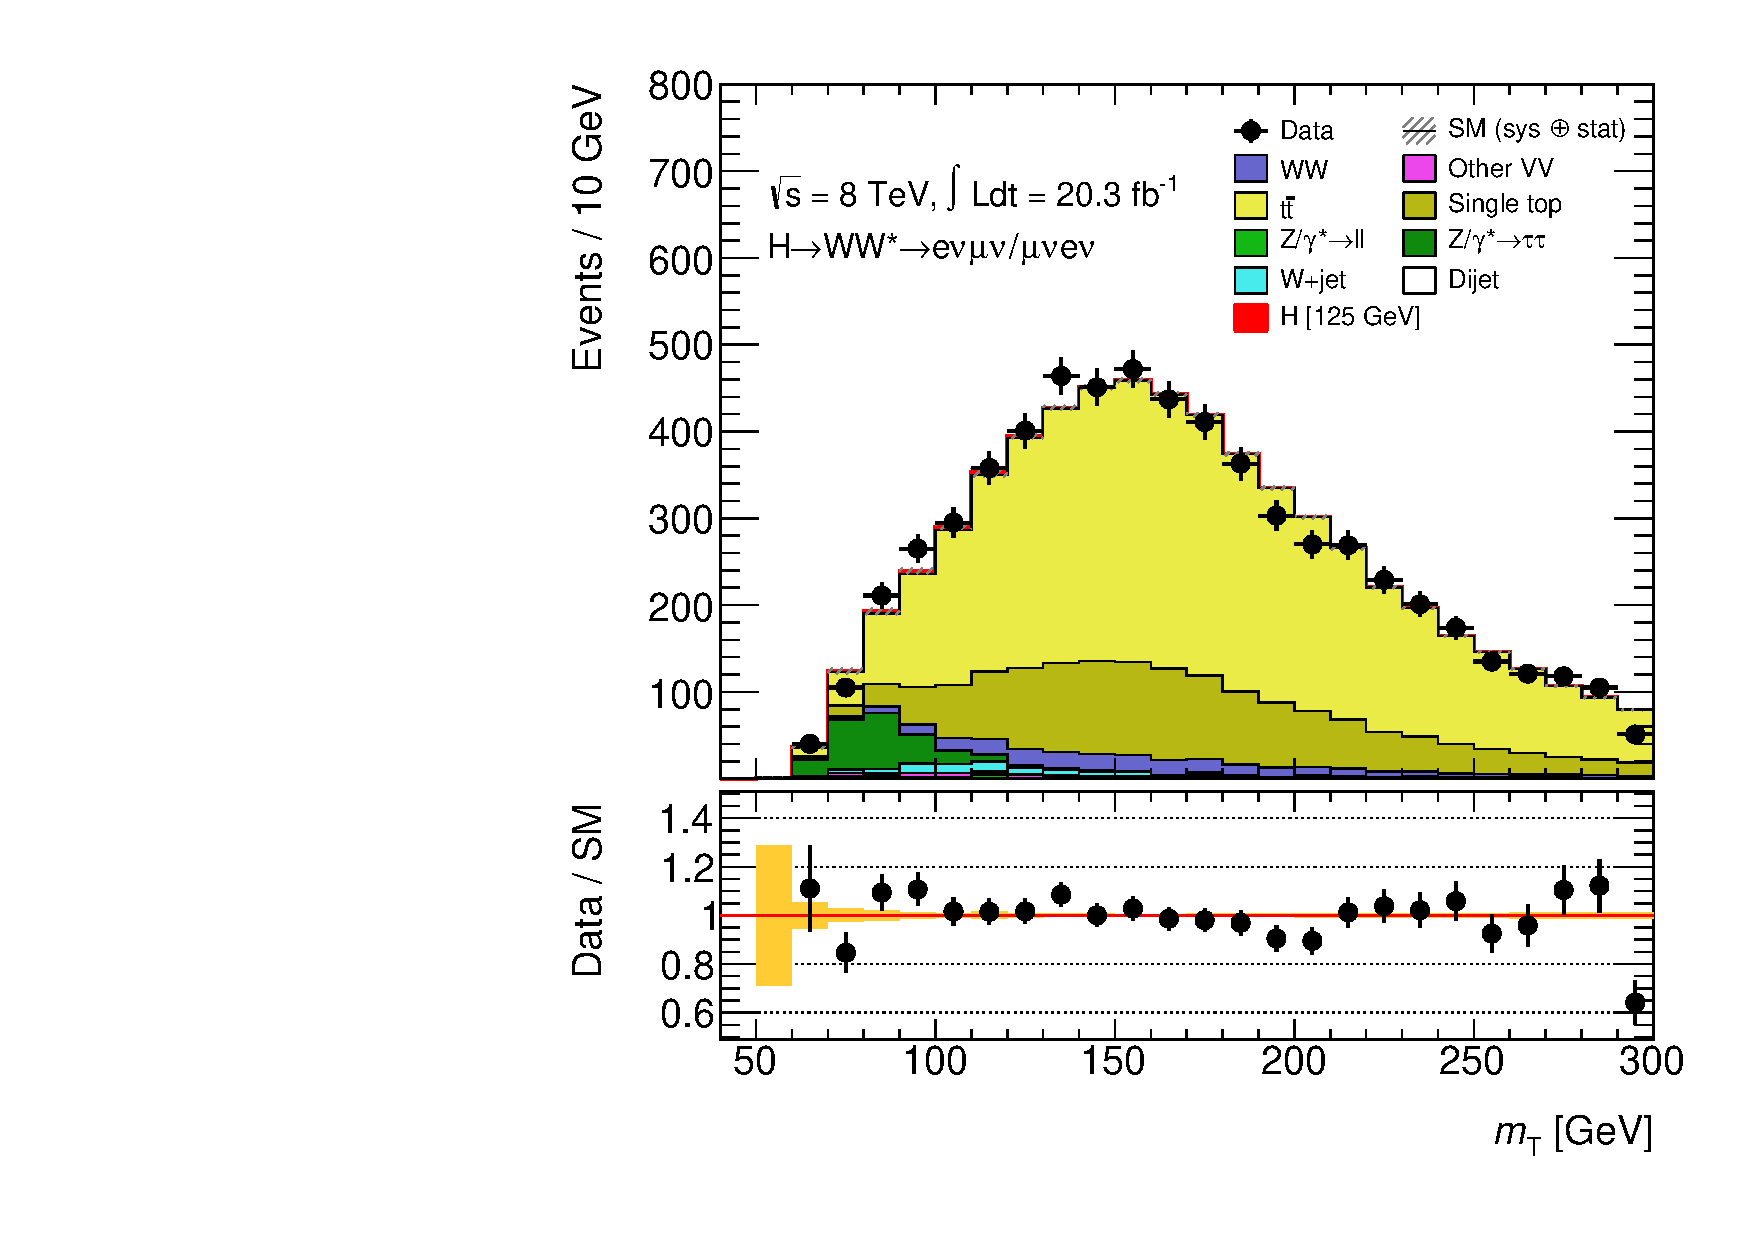
\includegraphics[width=0.495\textwidth]{tex/backgrounds/emme_CutMTW_1j_noSubBjet_Btagged_MT_TrackHWW_Clj_mh125_lin}
	\hfill
	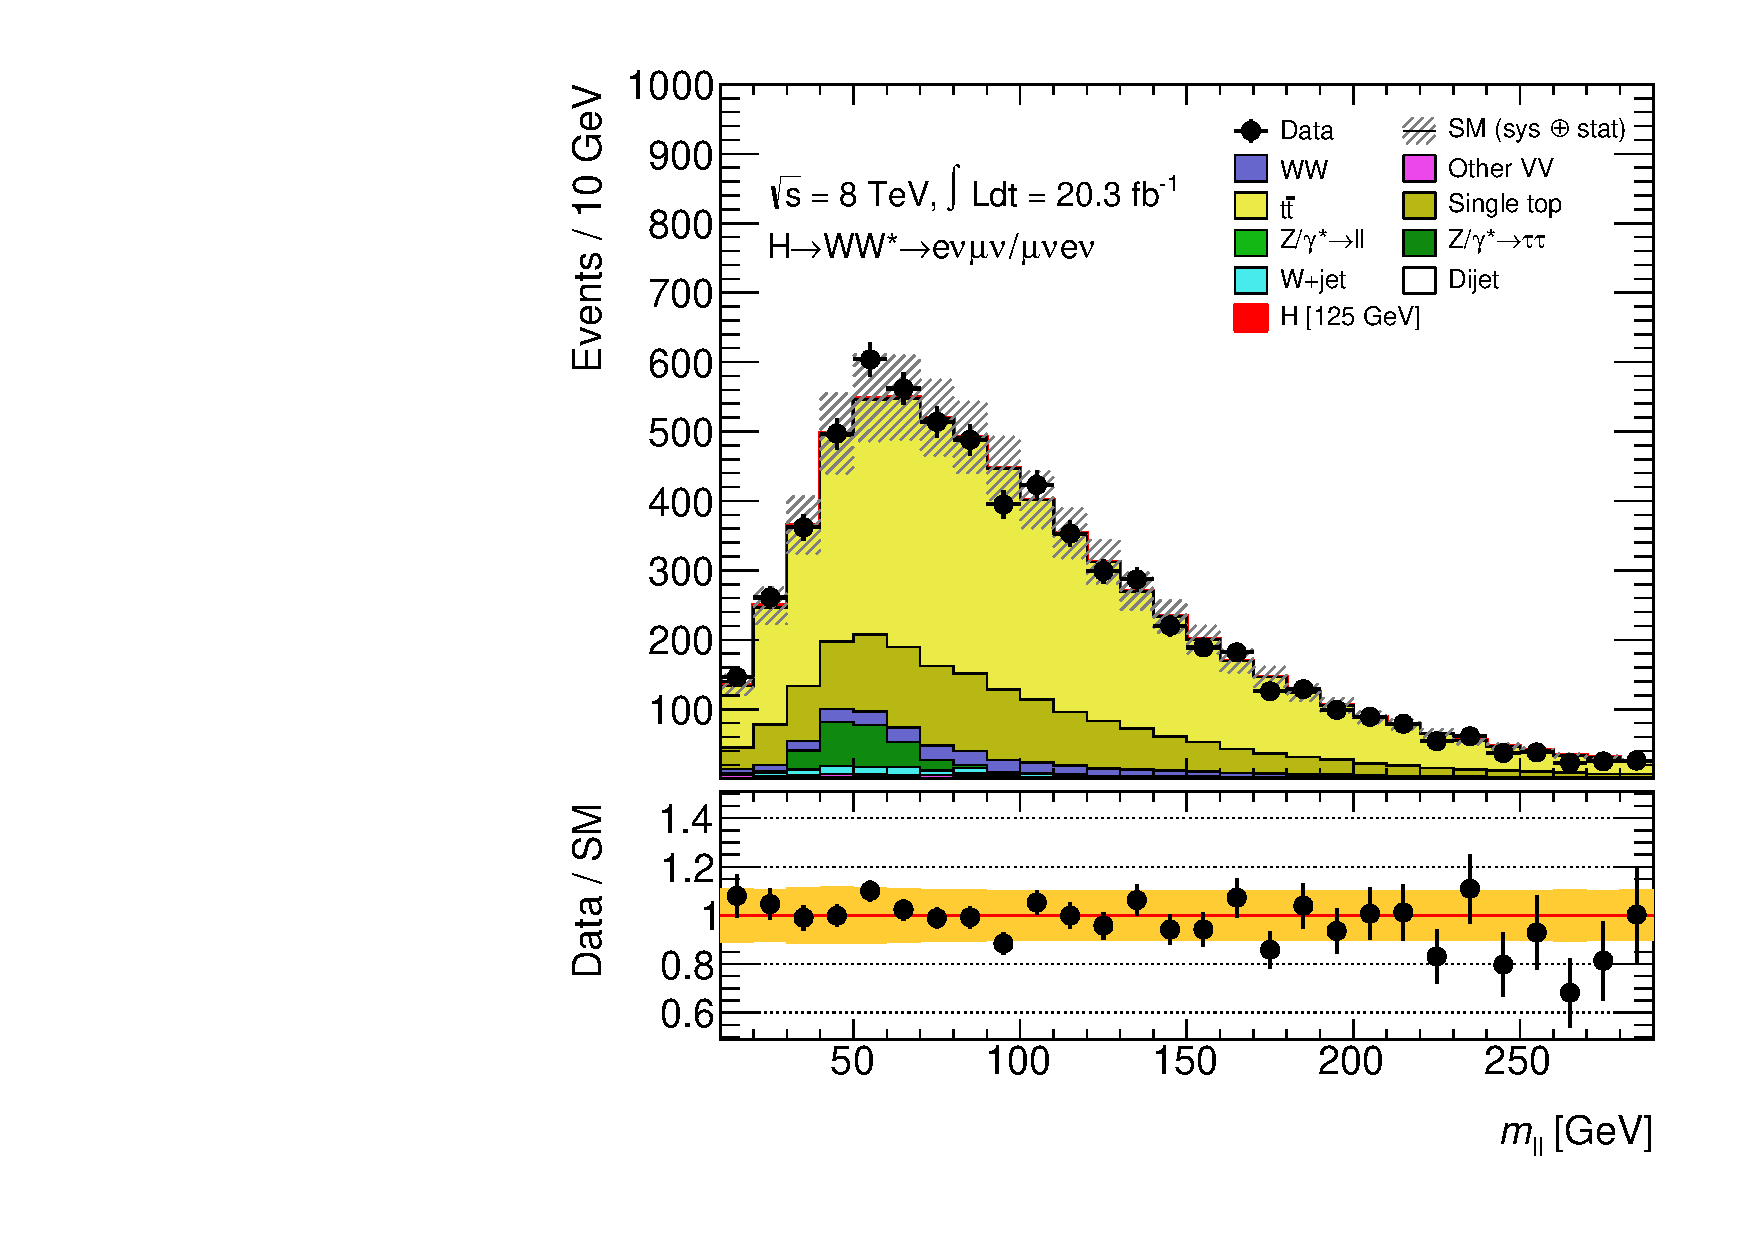
\includegraphics[width=0.495\textwidth]{tex/backgrounds/emme_CutMTW_1j_noSubBjet_Btagged_Mll_mh125_lin}
	\caption{The \mt (left) and \mll (right) distributions for events passing the 
	pre-selection and containing 1 jet and 1 \Pbottom-tagged jet. The jet \Pbottom-tagging 
	efficiency extrapolation method uses the top normalisation in this region and 
	extrapolates to events with 0 \Pbottom-tagged jets. Normalisation factors are applied.}
	\label{fig:top:jbee}
\end{figure}

The \Pbottom-tagging efficiency of jets in top events $\varepsilon_{\Pbottom}$ is measured 
in a high-purity top control region (CR). These events pass the pre-selection (minus the 
\corrtrackmet cut) and feature two jets, at least one of which is \Pbottom-tagged. 
$\varepsilon_{\Pbottom}$ is then measured using a tag-and-probe method, where the tag is a 
\Pbottom-tagged jet and the probe is the other jet. Since $\varepsilon_{\Pbottom}$ is 
measured in 2-jet events but applied to 1-jet events, an MC-based correction is applied to 
the measured \Pbottom-tagging efficiency
\begin{equation}
	\varepsilon_{\Pbottom}^{\text{pred,ESR,1j}} = \frac{\varepsilon_{\Pbottom}^{\text{MC,ESR,1j}}}{\varepsilon_{\Pbottom}^{\text{MC,CR,2j}}} \cdot \varepsilon_{\Pbottom}^{\text{data,CR,2j}} \,.
	\label{eq:top:jbee}
\end{equation}

The total uncertainty in the expected 1-jet top background is \about6.8\%, dominated by 
theoretical uncertainties in the MC-based correction to $\varepsilon_{\Pbottom}$ in 
(\ref{eq:top:jbee}).

To estimate the top background in 1-jet regions other than the SR, the method is viewed as 
providing a simple data-driven normalisation factor. This is equivalent to neglecting the 
extrapolation uncertainties, but is helpful when plotting observables. The normalisation 
factor is measured to be \stat{1.042}{0.025}\todo{update}.



\subsection{\twojet bin estimation}
\label{sec:top:2j}

As in the 1-jet bin, a veto on \Pbottom-tagged jets rejects the majority of the top 
background. However, even after this veto, top remains the largest background in the 
\twojet bin. Fortunately, this enables a top control region (CR) to be defined which 
includes the \Pbottom-tagged jet veto, greatly reducing the uncertainties due to 
\Pbottom-tagging efficiencies.

The top CR is defined in a high-\mll region, similarly to the \WW CRs in the 0-jet and 
1-jet bins. It is defined by the same criteria as the \twojet SR (minus the \mtautau, 
\dphill and \VH cuts), but the \mll cut is changed to \unit{$\mll > 80$}{\GeV}. The 
observed number of events is then extrapolated to the signal region (SR) using MC
\begin{equation}
	N_{\text{top}}^{\text{pred,SR}} &= \alpha_{\text{top}}^{\geq2\text{j}} \parenths{N^{\text{data,CR}} - N_{\text{non-top}}^{\text{pred,CR}}} \\
	\alpha_{\text{top}}^{\geq2\text{j}} &= N_{\text{top}}^{\text{MC,SR}} / N_{\text{top}}^{\text{MC,CR}} \,.
\end{equation}
The uncertainty is dominated by theoretical uncertainties in the extrapolation 
$\alpha_{\text{top}}^{\geq2\text{j}}$.

\begin{figure}[t]
	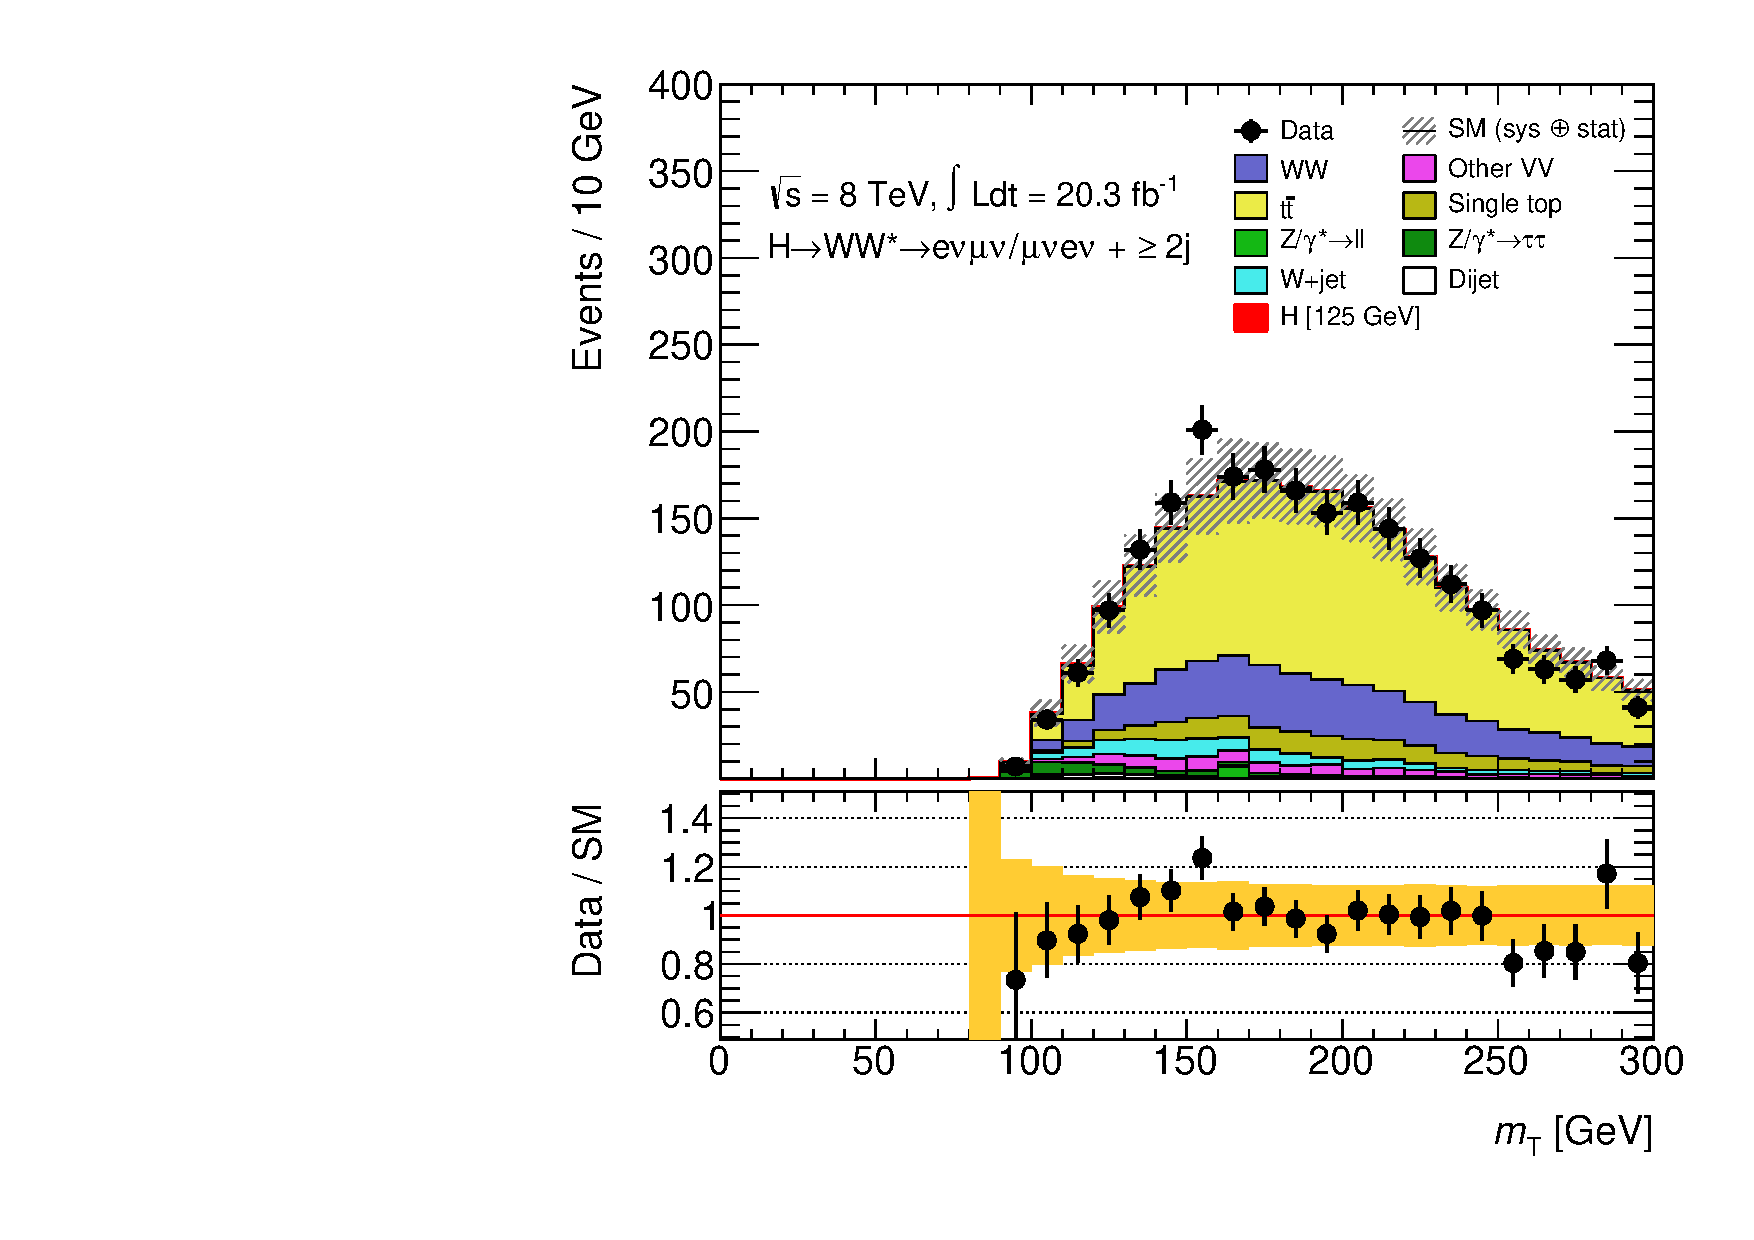
\includegraphics[width=0.495\textwidth]{tex/backgrounds/emme_CutFailVBFHighMllTopCR_2jetincl_MT_TrackHWW_Clj_mh125_lin}
	\hfill
	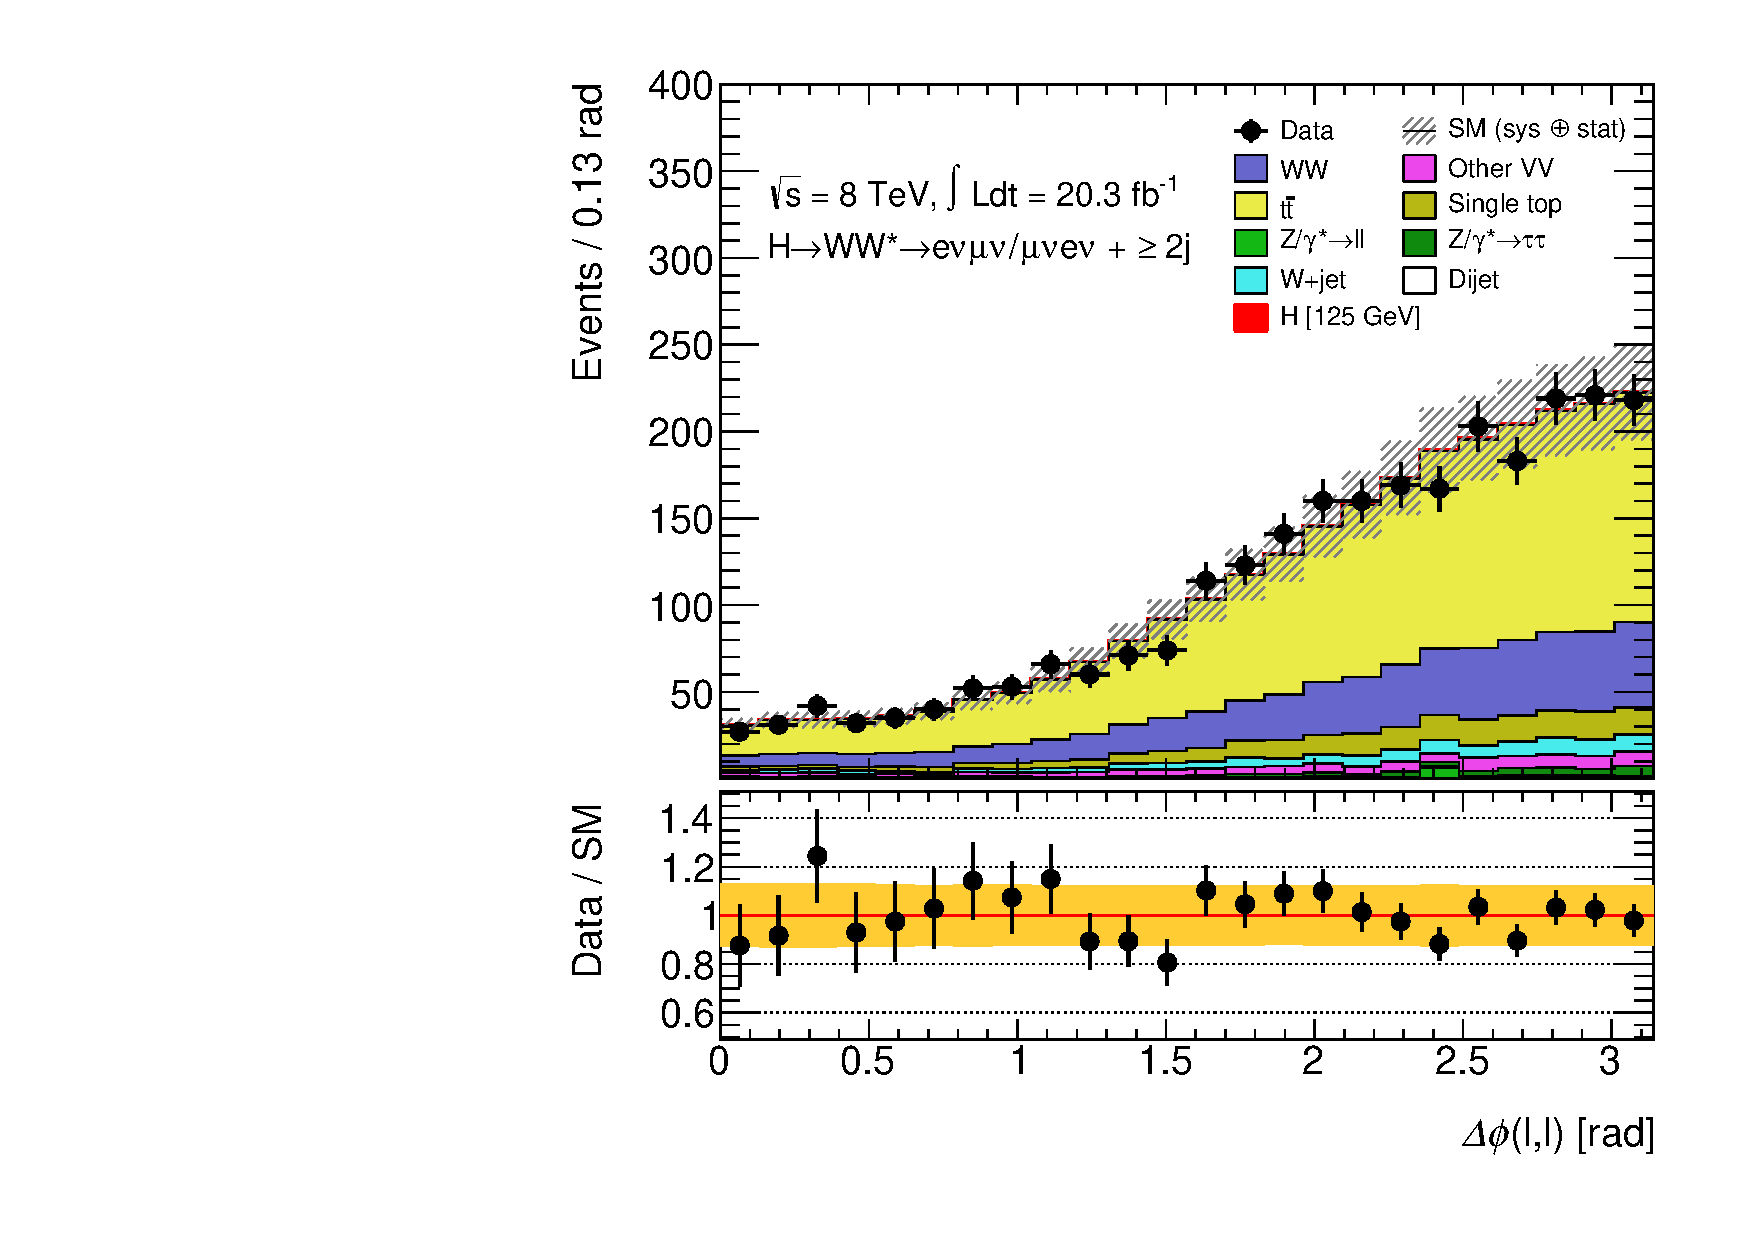
\includegraphics[width=0.495\textwidth]{tex/backgrounds/emme_CutFailVBFHighMllTopCR_2jetincl_DPhill_mh125_lin}
	\caption{The \mt (left) and \dphill (right) distributions in the top control region of 
	the \twojet bin. Normalisation factors are applied.}
	\label{fig:top:2j}
\end{figure}

To estimate the top background in \twojet regions other than the SR, the method is viewed 
as providing a simple data-driven normalisation factor. This is equivalent to neglecting 
the extrapolation uncertainties, but is helpful when plotting observables. The 
normalisation factor is measured to be \stat{1.078}{0.030}\todo{update}. 
\Figure~\ref{fig:top:2j} shows the good description of experimental data in the CR, 
after application of the normalisation factors.


\section{\DY}
	\label{sec:dy}
	%!TEX root = ../../thesis.tex

The \DY background is naturally split into \DYll and \DYtt processes. The former 
contributes almost exclusively to the \eech/\mmch channels,\footnote{
	In rare cases, \DYll events can enter the \emch/\mech channels. For example 
	\HepProcess{\DY \HepTo \Pmu\Pmu\Pphoton}, where a muon radiates a photon which 
	subsequently converts and is reconstructed as an electron.
}
where it is the dominant background. The latter can contribute to any channel since the 
two \HepProcess{\Ptau \HepTo \Plepton\Pnulepton\Pnut} decays are independent, though is 
doubly suppressed by the small $\text{BR}\parenths{\HepProcess{\Ptau \HepTo 
\Plepton\Pnulepton\Pnut}} = 17.6\%$ \cite{PDG:2012}.

Although \DYll does not feature prompt neutrinos, degradation of the \met resolution due 
to high pile-up can cause some \DYll events to exhibit significant \met. Since this is a 
difficult effect to model and \DYll is the dominant background to the \eech/\mmch 
channels, a high threshold of \unit{$\metrel > 40$}{\GeV} is used in the pre-selection. 
This is further tightened by tracker-based \trackmetrel cuts. On the other hand, \DYtt 
does feature prompt neutrinos and is suppressed by other cuts, such as the \mtautau veto.

The \DY backgrounds are estimated by data-driven techniques, in combination with MC 
modelling provided by \meps{\alpgen}{\fherwig}. Overlap between the \DY MC and the 
\Zgamma MC is removed through careful consideration of the MC event records.



\subsection{\DY boson transverse momentum}
\label{sec:dy:pt}

Selecting \eech/\mmch events with \unit{$\mods{\mll - \mZ} < 15$}{\GeV} results in a very 
pure sample of \DYll events, enabling the MC to be validated. In doing so, the \ptll 
distribution is found to be poorly modelled at \unit{$\ptll > 30$}{\GeV} in the 0-jet 
bin (see \Figure~\ref{fig:dy:ptZ_reweight}), despite being well modelled inclusively. 
This is unsurprising since a difficult phase space, sensitive to soft hadronic activity 
and jet shapes, has been selected: requiring a highly boosted \DY boson whilst vetoing 
events with jets. It is important to model \ptll accurately, as other observables such as 
\dphill and \ptleadlep are correlated.

For this reason, a data-driven correction to the \ptZ distribution is employed. It is 
derived in \mmch 0-jet events with \unit{$\mods{\mll - \mZ} < 15$}{\GeV}, by 
comparing the \ptll distribution observed in experimental data to that predicted by 
uncorrected MC. Each 0-jet MC event is then weighted according to its hadron-level \ptZ. 
This is found to improve the modelling of detector-level observables such as \ptll, 
\dphill and \ptleadlep (see \Figure~\ref{fig:dy:ptZ_reweight}). This correction is 
applied to the \HepProcess{\DY \HepTo \Pe\Pe/\Pmu\Pmu/\Ptau\Ptau} processes, though only 
to the 0-jet bin.

\begin{figure}[p]
	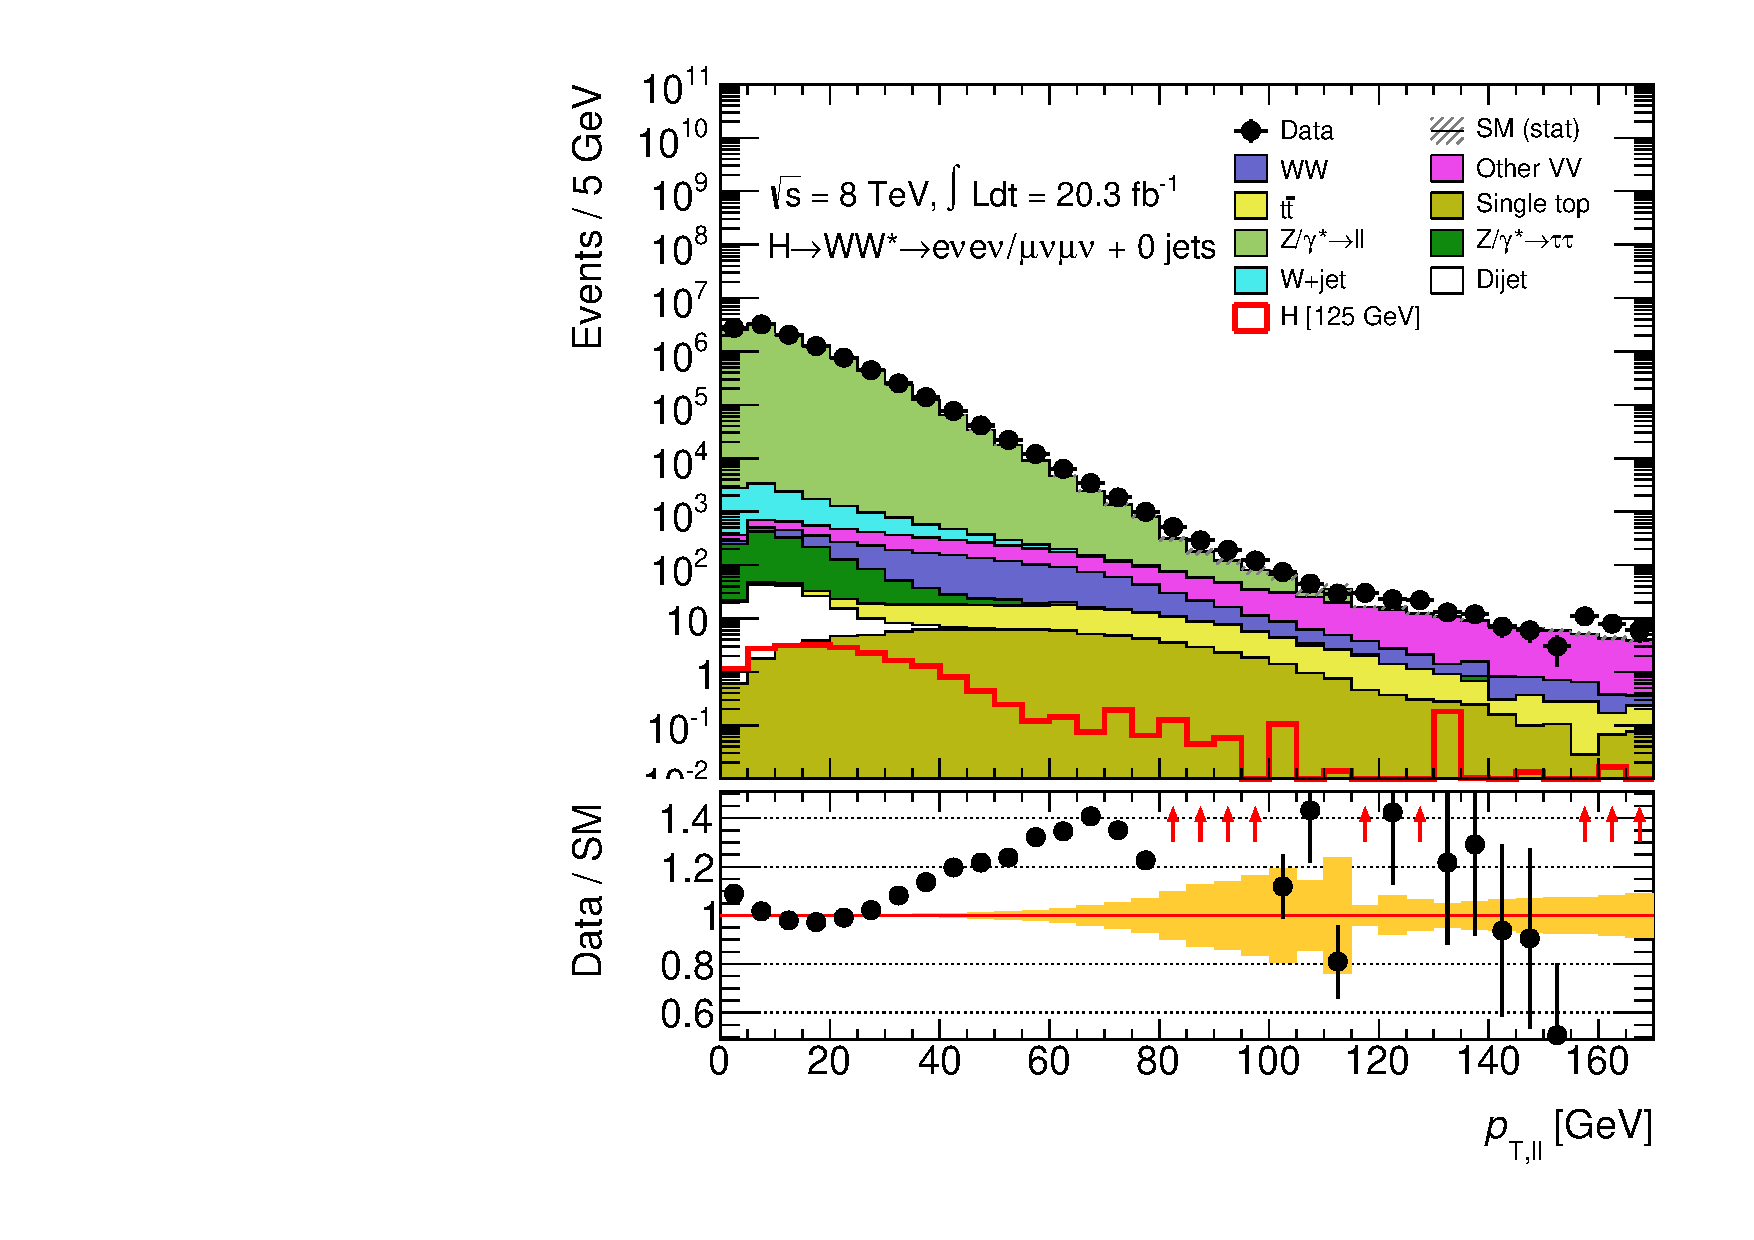
\includegraphics[width=0.48\textwidth]{tex/backgrounds/ZpT-off/eemm_CutZControl_0jet_Ptll_mh125_log}
	\hfill
	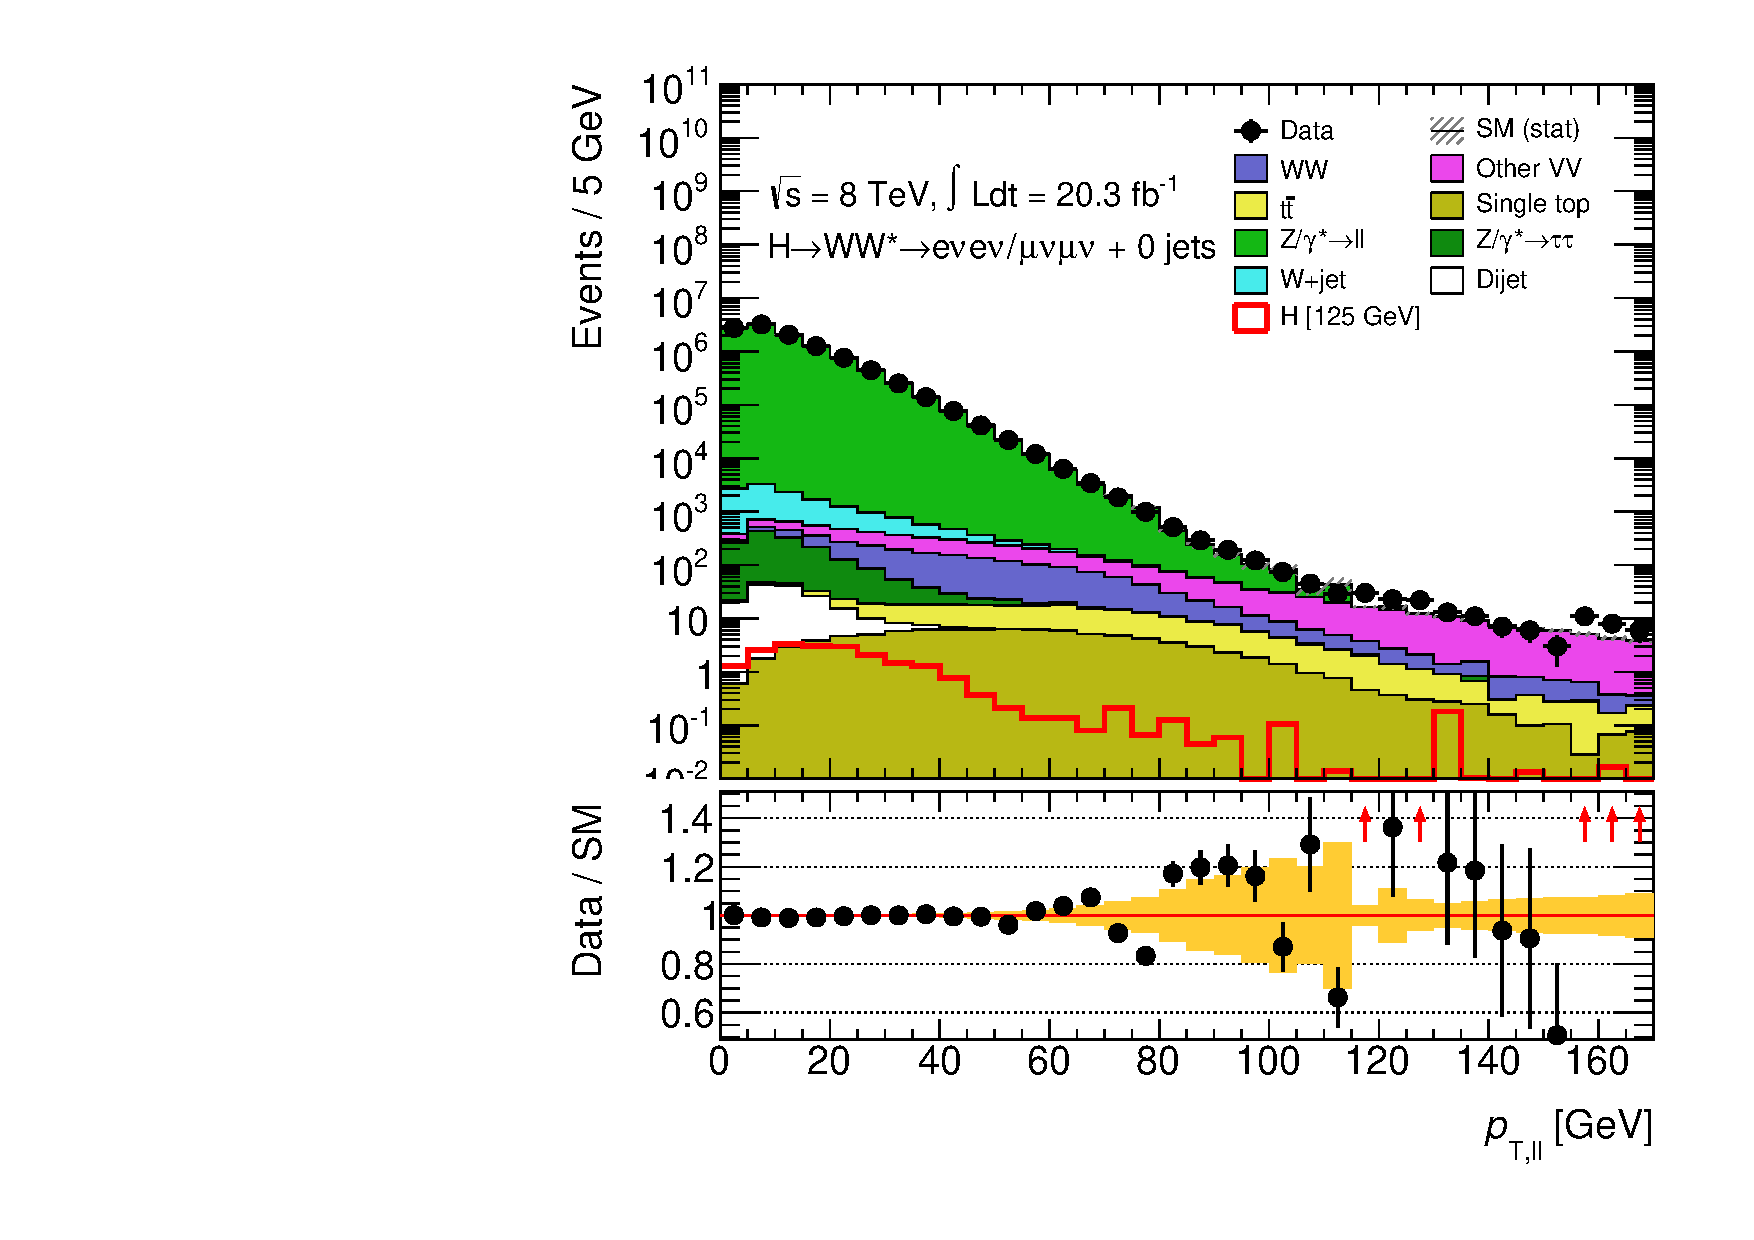
\includegraphics[width=0.48\textwidth]{tex/backgrounds/ZpT-on/eemm_CutZControl_0jet_Ptll_mh125_log}
	\\
	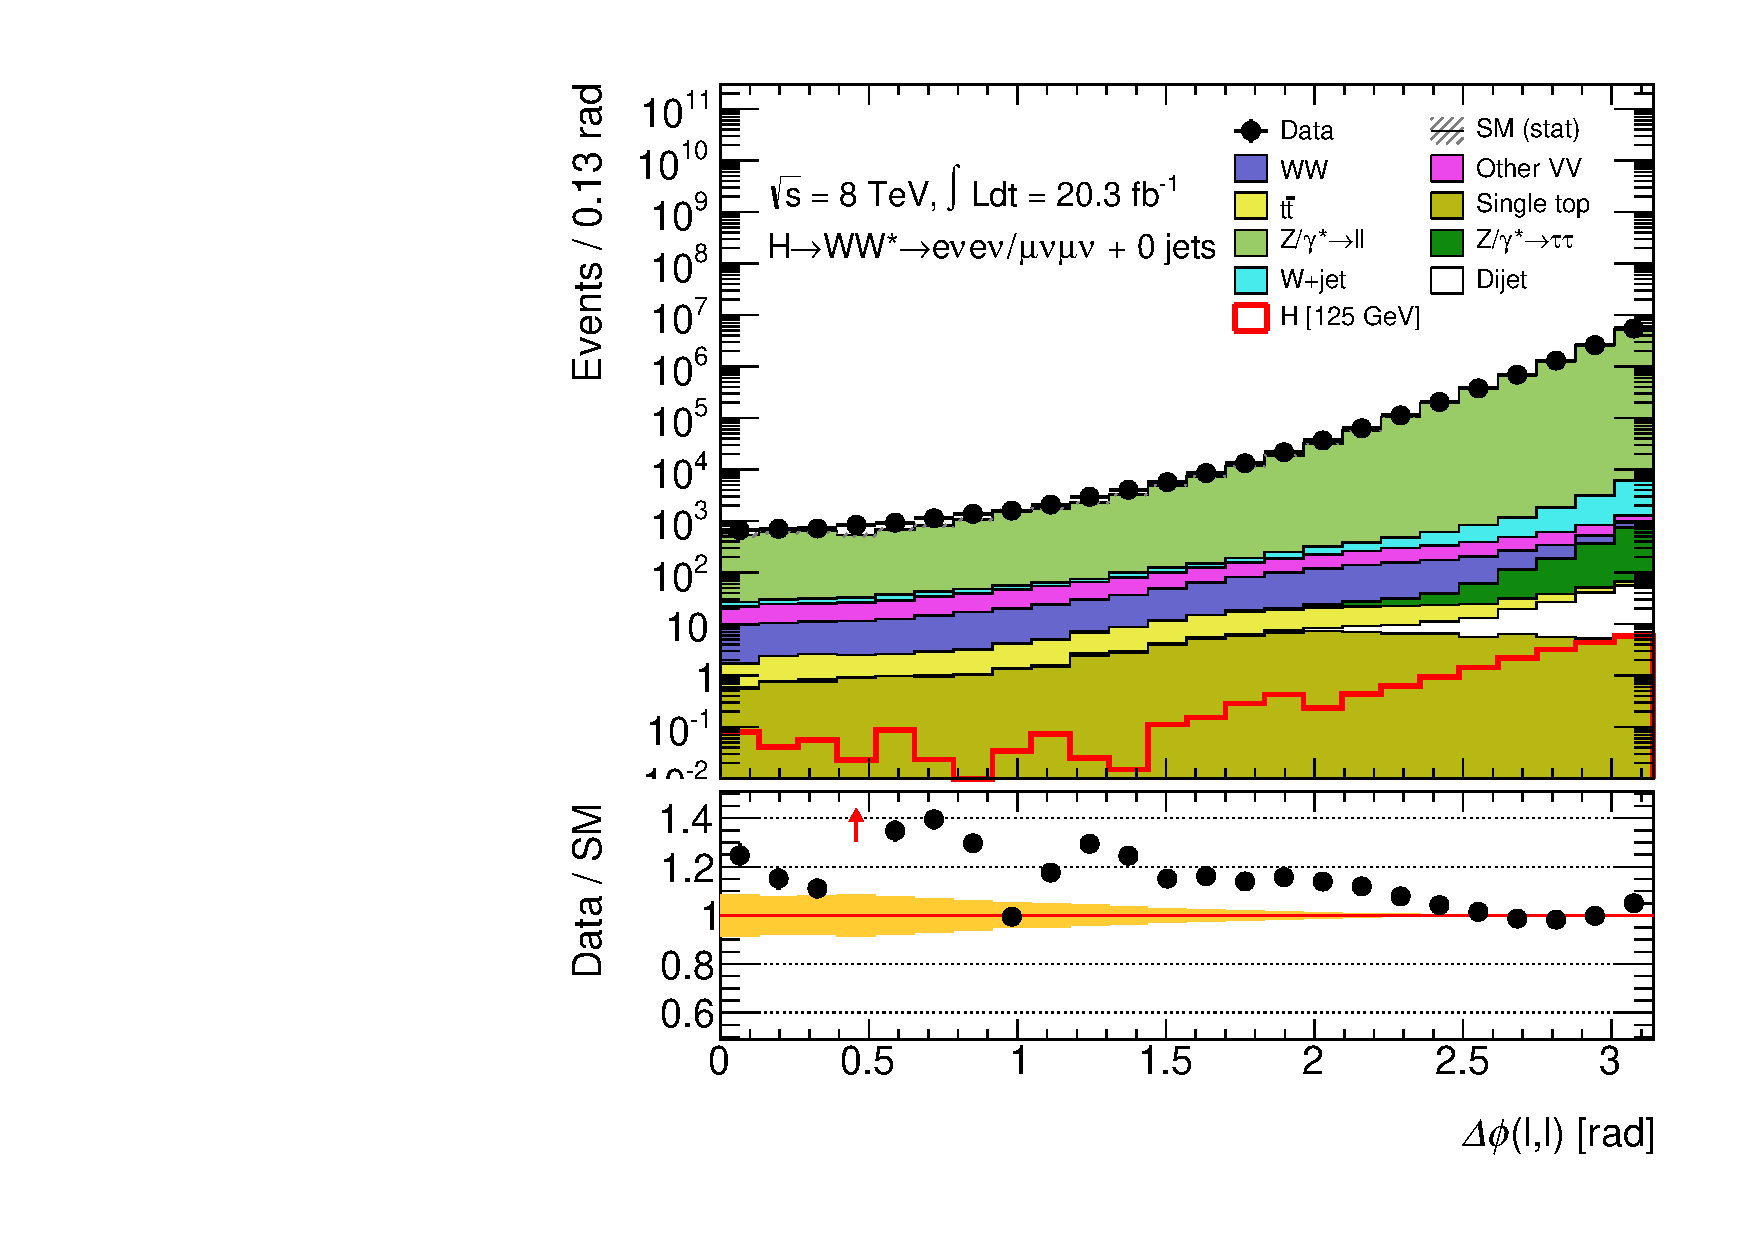
\includegraphics[width=0.48\textwidth]{tex/backgrounds/ZpT-off/eemm_CutZControl_0jet_DPhill_mh125_log}
	\hfill
	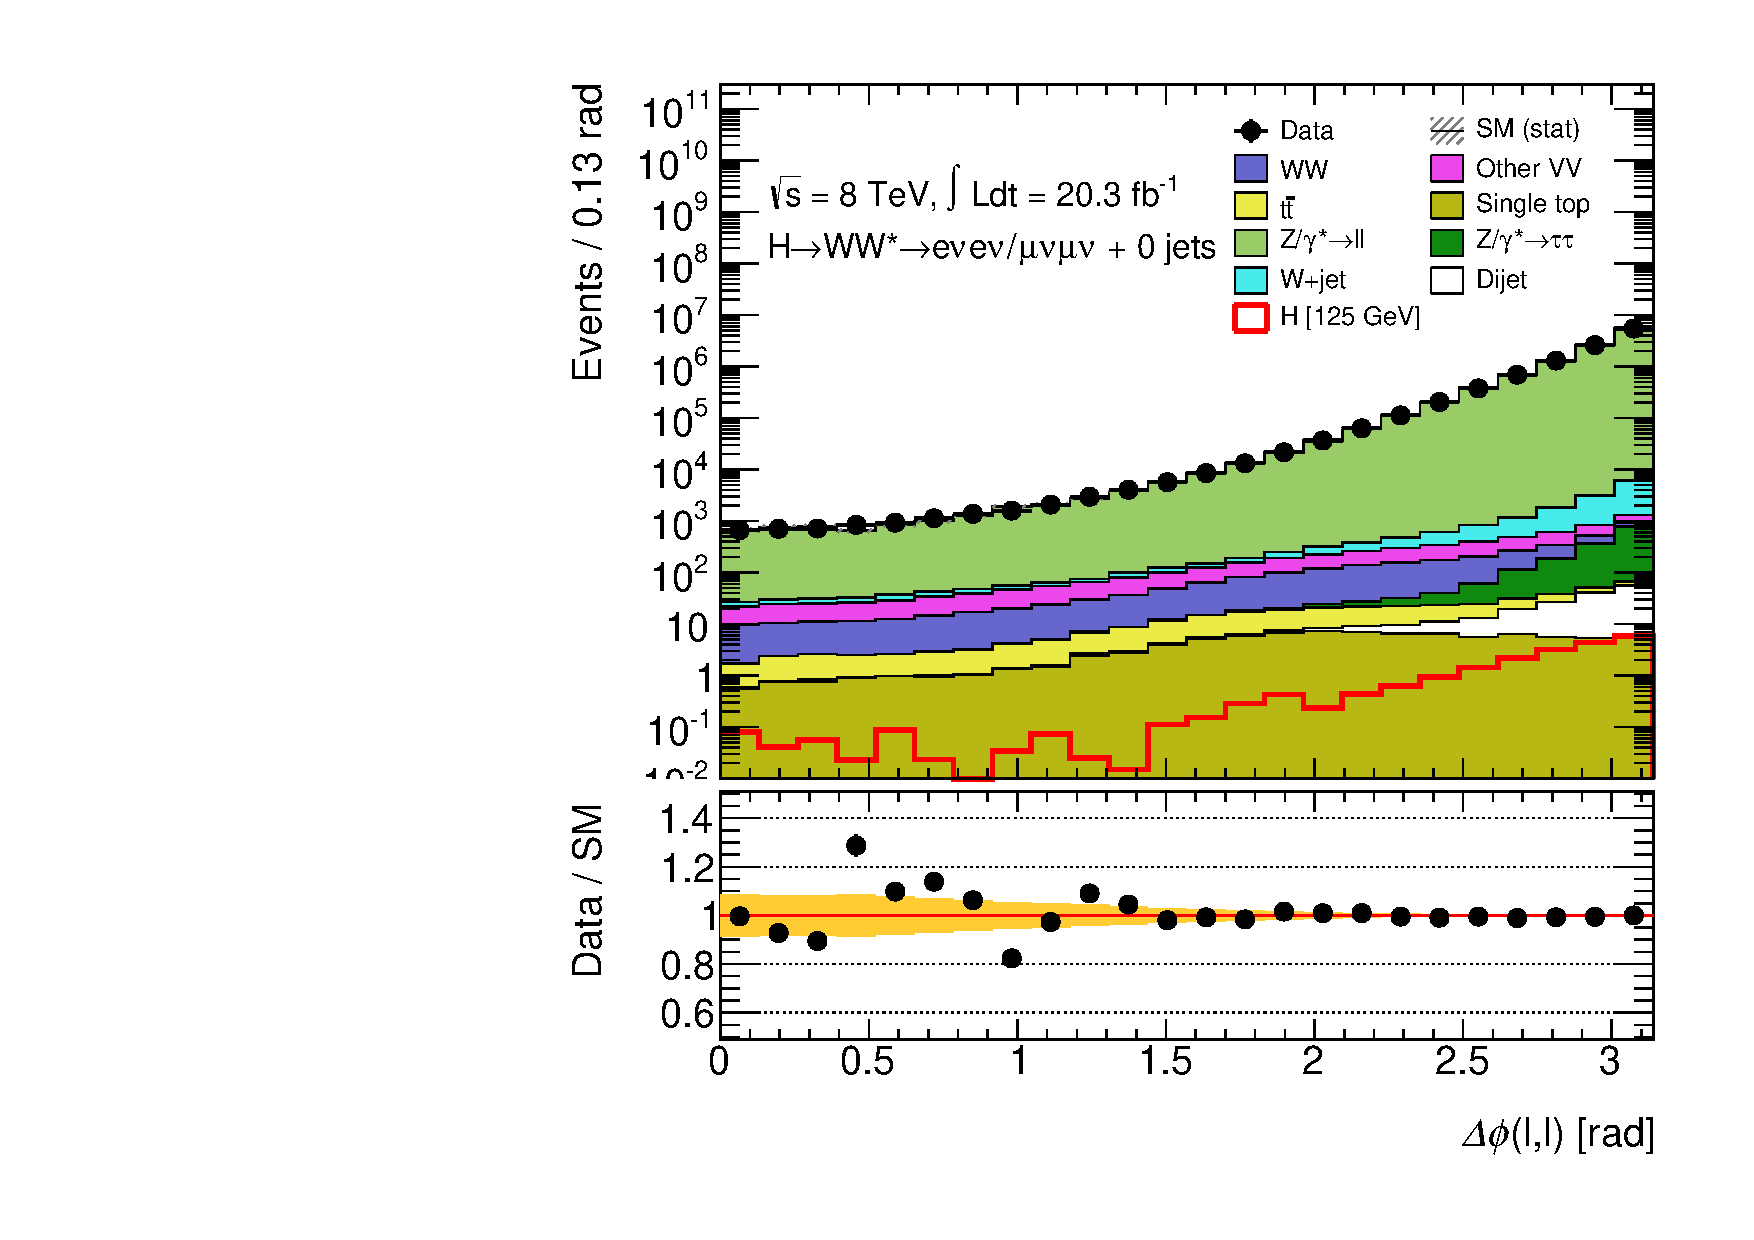
\includegraphics[width=0.48\textwidth]{tex/backgrounds/ZpT-on/eemm_CutZControl_0jet_DPhill_mh125_log}
	\\
	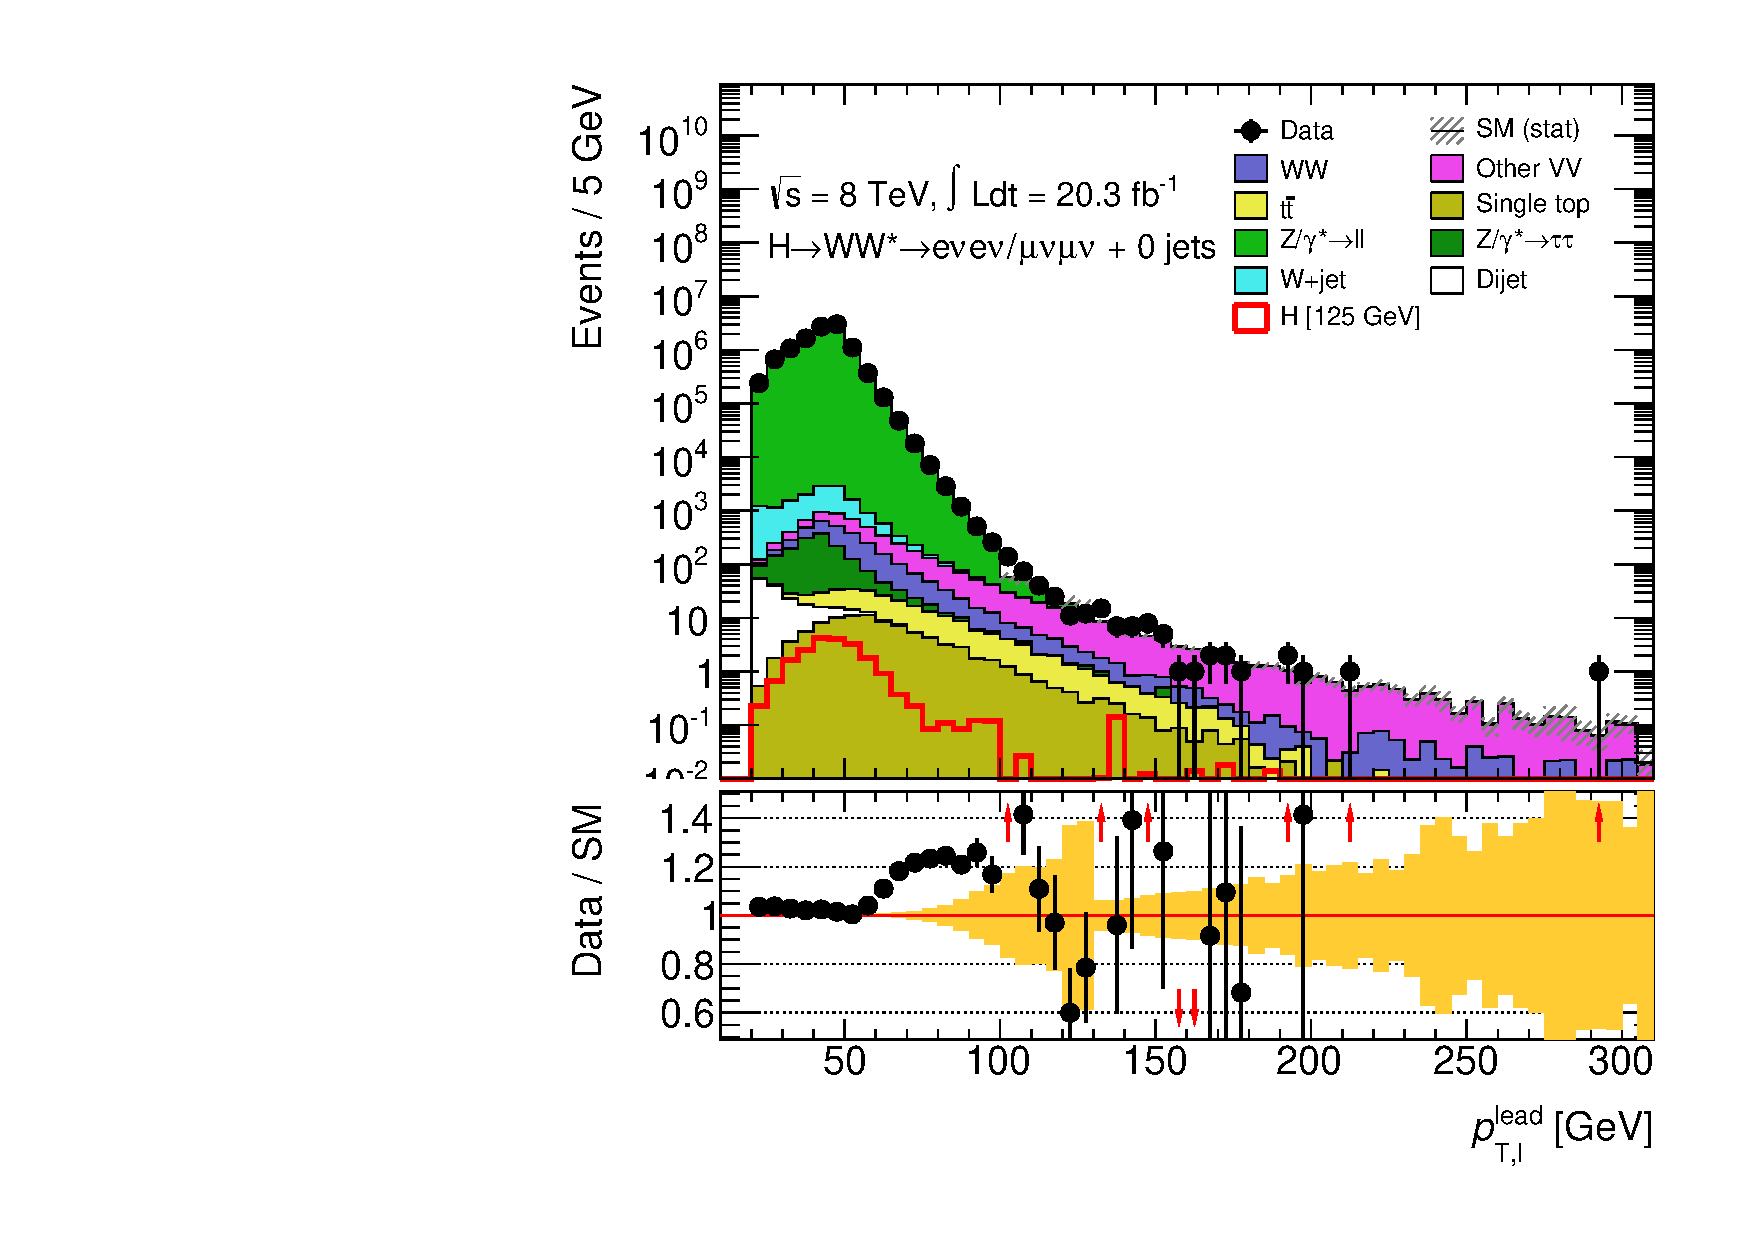
\includegraphics[width=0.48\textwidth]{tex/backgrounds/ZpT-off/eemm_CutZControl_0jet_lepPtLead_mh125_log}
	\hfill
	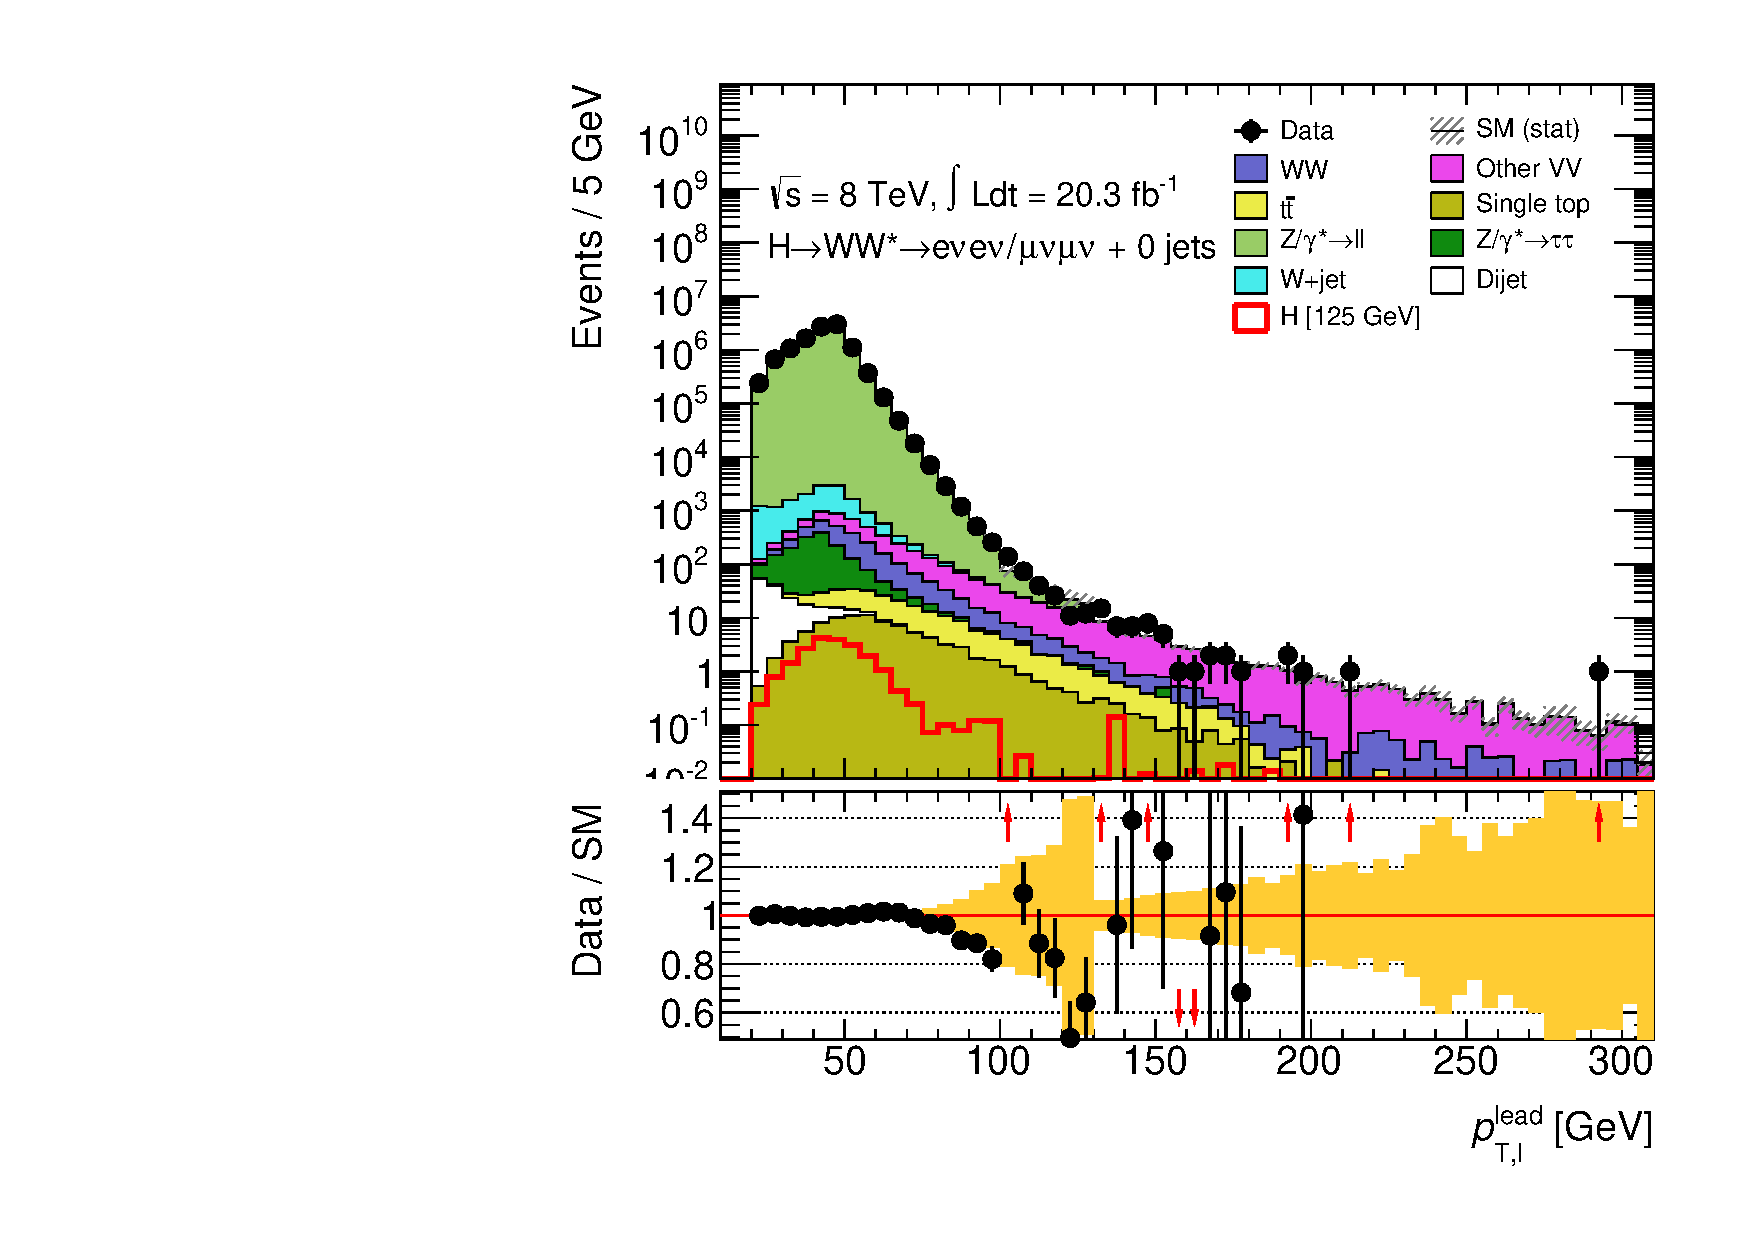
\includegraphics[width=0.48\textwidth]{tex/backgrounds/ZpT-on/eemm_CutZControl_0jet_lepPtLead_mh125_log}
	\caption{Leptonic distributions in the 0-jet \DYll control region, before (left) and 
	after (right) the \ptZ correction is applied.}
	\label{fig:dy:ptZ_reweight}
\end{figure}

The \ptZ mismodelling might be different in the signal region to the \PZ control region 
where it is derived. The validity of this extrapolation of the correction was tested by 
deriving similar corrections to \sherpa (instead of experimental data). This indicated 
there is a correlation between the correction and the \met requirement. Thus, another 
correction is derived with an additional \unit{$\corrtrackmet > 20$}{\GeV} cut, which is 
used to estimate the uncertainty in the correction.



\subsection{\DYtt estimation}
\label{sec:dy:tautau}

The \DYtt background is measured in a dedicated control region (CR), and then 
extrapolated to the signal region (SR) using MC
\begin{equation}
	N_{\HepProcess{\PZ\HepTo\Ptau\Ptau}}^{\text{pred,SR}} &= \alpha_{\HepProcess{\PZ\HepTo\Ptau\Ptau}} \cdot \parenths{N^{\text{data,CR}} - N_{\text{non-}\HepProcess{\PZ\HepTo\Ptau\Ptau}}^{\text{pred,CR}}} \\
	\alpha_{\HepProcess{\PZ\HepTo\Ptau\Ptau}} &= N_{\HepProcess{\PZ\HepTo\Ptau\Ptau}}^{\text{MC,SR}} / N_{\HepProcess{\PZ\HepTo\Ptau\Ptau}}^{\text{MC,CR}} \,.
\end{equation}
A control region is defined for each jet bin in the \emch/\mech channels, as shown in 
\Table~\ref{tab:dytt_cr_sel}. These are used to extrapolate to the respective signal 
regions, for all channels.

\todo[inline]{Plot CR}

\begin{table}[t]
	\begin{tabularx}{0.7\textwidth}{YYY}
		\toprule
		\multicolumn{3}{c}{\emch/\mech} \\
		\midrule
		\multicolumn{3}{c}{$\ptleadlep > 22$ and $\ptsubleadlep > 10$} \\
		\multicolumn{3}{c}{$\mll > 12$} \\
		\multicolumn{3}{c}{$\corrtrackmet > 20$} \\
		\cmidrule(lr){1-3}
		0-jet bin & 1-jet bin & \twojet bin \\
		\cmidrule(lr){1-3}
		-- & $\nbjets = 0$ & $\nbjets = 0$ \\
		-- & $\maxmtw > 50$ & -- \\
		-- & $\mtautau > \mZ - 25$ & -- \\
		-- & -- & Fail CJV or OLV \\
		$\mll < 80$ & $\mll < 80$ & $\mll < 70$ \\
		$\dphill > 2.8$ & -- & $\dphill > 2.8$ \\
		\bottomrule
	\end{tabularx}
	\caption{Event selection criteria of the \DYtt control regions. Cuts on energy, 
	momentum and mass are given in \GeV, and angular cuts are given in radians. The 
	relevant variables are described in 
	\Chapter~\ref{chap:selection}.}
	\label{tab:dytt_cr_sel}
\end{table}

The corresponding normalisation factors are \stat{1.01}{0.02} in the 0-jet bin, 
\stat{1.08}{0.04} in the 1-jet bin, and \stat{1.05}{0.10} in the \twojet bin.



\subsection{\DYll estimation}
\label{sec:dy:ll}

\DYll is the dominant background to the \eech/\mmch channels, and this section will 
describe how it is estimated in the corresponding 0-jet and 1-jet bins (the \twojet bin 
is unused in the \eech/\mmch channels).

\DYll is largely rejected by the \PZ boson mass veto, 
\unit{$\mods{\mll - \mZ} > 15$}{\GeV}, and the requirement of large missing transverse 
momentum, \unit{$\metrel > 40 (40)$}{\GeV} and \unit{$\trackmetrel > 40 (35)$}{\GeV} in 
the 0-jet (1-jet) bin. Although the \met resolution is broadened by pile-up, for 
surviving events to possess such high \metrel and \trackmetrel suggests some mismeasured 
hadronic activity recoiling against the dilepton (+ jet) system. This is also enhanced 
by the \unit{$\ptll > 30$}{\GeV} cut in the 0-jet bin.

This hadronic recoil must be soft and broad in order to avoid passing the jet 
reconstruction, and might not be modelled accurately. It is therefore preferable to use 
a data-driven estimation of this background. Fortunately, the \frecoil observable 
(described below) can discriminate \DYll from other processes in this phase space, and 
can simultaneously be used to suppress and estimate the \DYll background.

First, soft jets with \unit{$\pt > 10$}{\GeV} and $\mods{\eta} < 4.5$ are found, 
following the jet selection detailed in \Section~\ref{sec:objects:jets} minus the JVF 
cut. In the 0-jet bin, \frecoil is defined by
\begin{equation}
	\frecoil = \left. \mods{\sum\limits_{j\text{ in }\wedge} \text{JVF}_{j} \cdot \bvec{p}_{\text{T,}j}} \, \middle/ \ptll \right.
	\label{eq:dy:frecoil}
\end{equation}
where $\wedge$ is the detector quadrant centred on $-\ptllvec$. This is the fraction of 
\ptll that can be balanced by soft hadronic activity in the opposing quadrant. 
In the 1-jet bin, it is the dilepton + jet system that must be balanced, and thus the 
quadrant $\wedge$ is centred upon $-\ptlljvec$ and the denominator becomes \ptllj.

The tight \met criteria sculpt \frecoil in \DYll towards higher values, whereas the other 
background processes (and signal) feature high-\pt neutrinos and peak at lower values 
(see \Figure~\ref{fig:dy:frecoil_shape}). A \textit{template method} exploits the 
markedly different \frecoil shape of the \DYll background to estimate its contribution to 
the \eech/\mmch signal regions.

\begin{figure}[t]
	
\includegraphics[width=0.495\textwidth]{tex/motivation/sombrero_comical}
	\hfill
	
\includegraphics[width=0.495\textwidth]{tex/motivation/sombrero_comical}
	\caption{\frecoil shape in the 0-jet (left) and 1-jet (right) signal regions of the 
	\eech/\mmch channels, excluding the \frecoil cut itself. The non-\DYll backgrounds 
	are modelled by data-driven methods described elsewhere, while the \DYll and signal 
	processes are described by MC.}
	\label{fig:dy:frecoil_shape}
\end{figure}

In the template method, the signal region (SR) is defined by the full event selection of 
the \eech/\mmch channels, excluding the \frecoil cut (whose efficiency shall be predicted 
by the method). The \frecoil distribution $\mathcal{T}$ in the SR of the same-flavour 
(SF) channels, \ie the \eech/\mmch channels, has two components with distinct shapes: 
\DYll and other processes (including signal). If the shape of both components are 
predicted, then their relative contributions can be fit using the observed \frecoil 
distribution in the SR
\begin{equation}
	\mathcal{T}^{\text{data,SR,SF}} = K^{\text{fit}}_{\text{non-}\HepProcess{\PZ\HepTo\Plepton\Plepton}} \cdot \mathcal{T}^{\text{pred,SR,SF}}_{\text{non-}\HepProcess{\PZ\HepTo\Plepton\Plepton}} + K^{\text{fit}}_{\HepProcess{\PZ\HepTo\Plepton\Plepton}} \cdot \mathcal{T}^{\text{pred,SR,SF}}_{\HepProcess{\PZ\HepTo\Plepton\Plepton}}
	\label{eq:dy:pacman_basic}
\end{equation}
where $K^{\text{fit}}_{i}$ are prefactors determined by the fitting procedure, and the 
input distributions $\mathcal{T}^{\text{pred,SR,SF}}_{i}$ are determined by data-driven 
methods described below.

$\mathcal{T}^{\text{pred,SR,SF}}_{\text{non-}\HepProcess{\PZ\HepTo\Plepton\Plepton}}$ 
is determined from the observed distribution in different-flavour (DF) events, \ie the 
\emch/\mech channels, $\mathcal{T}^{\text{data,SR,DF}}$. Note that this DF distribution 
is measured in the SR defined by SF event selection criteria. In doing this, the 
normalisation factor $K^{\text{fit}}_{\text{non-}\HepProcess{\PZ\HepTo\Plepton\Plepton}}$ 
becomes an extrapolation parameter 
$\alpha_{\text{non-}\HepProcess{\PZ\HepTo\Plepton\Plepton}}^{\text{fit}}$ from DF to SF. 
This method is valid because the \DYll background to the SF channels is negligible, and 
the composition of the other processes is consistent between DF and SF events.

$\mathcal{T}^{\text{pred,SR,SF}}_{\HepProcess{\PZ\HepTo\Plepton\Plepton}}$ is determined 
from the SF distribution measured in a \DYll control region (CR) 
$\mathcal{T}^{\text{data,SR,DF}}$. The CR is defined by the same selection criteria as 
the SR, except that the \unit{$\mll < 55$}{\GeV} criteria becomes 
\unit{$\mods{\mll - \mZ} < 15$}{\GeV}. As the \met and \ptll criteria remain in the CR 
definition, \frecoil is sculpted similarly to the SR. However, this also means that the 
contribution of other processes in the CR is non-negligible and must be subtracted. This 
contamination is estimated from the distribution measured in DF events passing the same 
CR selection $\mathcal{T}^{\text{data,CR,DF}}$, with the extrapolation from DF to SF 
predicted by dedicated data-driven methods described elsewhere or by MC.

Thus, (\ref{eq:dy:pacman_basic}) becomes
\begin{equation}
	\mathcal{T}^{\text{data,SR,SF}} = \alpha_{\text{non-}\HepProcess{\PZ\HepTo\Plepton\Plepton}}^{\text{fit}} \cdot \mathcal{T}^{\text{data,SR,DF}} + \alpha_{\HepProcess{\PZ\HepTo\Plepton\Plepton}}^{\text{fit}} \cdot \parenths{\mathcal{T}^{\text{data,CR,SF}} - \alpha_{\text{non-}\HepProcess{\PZ\HepTo\Plepton\Plepton}}^{\text{pred}} \cdot \mathcal{T}^{\text{data,CR,DF}}}
	\label{eq:dy:pacman_full}
\end{equation}
where $\alpha_{\text{non-}\HepProcess{\PZ\HepTo\Plepton\Plepton}}^{\text{fit}}$ and 
$\alpha_{\text{non-}\HepProcess{\PZ\HepTo\Plepton\Plepton}}^{\text{pred}}$ are 
extrapolations from DF to SF, and 
$\alpha_{\HepProcess{\PZ\HepTo\Plepton\Plepton}}^{\text{fit}}$ is an extrapolation in 
\mll. Note that the $\alpha_i$ are prefactors and leave template shapes unchanged. The 
sensitivity of this method to the signal strength is tested and found to be negligible. 

The final event selection criterion in the \eech/\mmch channels is $\frecoil < 0.1$. The 
efficiency of this cut for both \DYll and other processes is inherently predicted by the 
template method. To simplify matters, the templates are reduced to two bins: 
$\frecoil < 0.1$ and $\frecoil > 0.1$. With two bins and two free parameters 
$\alpha^{\text{fit}}_i$, the system can be solved exactly. The dominant uncertainty in 
the 0-jet \DYll estimation arises from correlations between \frecoil and \mll, and is 
evaluated with MC to be 32\%. The 1-jet bin is dominated by statistical uncertainties.


\section{Summary of normalisation factors}
	\label{sec:NFs}
	%!TEX root = ../../thesis.tex

It is helpful to express the data-driven estimations of several backgrounds in terms of a 
normalisation factor, which is the ratio of the data-driven predicted yield to the MC-only 
predicted yield. Their pre-fit and post-fit values are summarised in 
\Table~\ref{tab:bkg:NFs}, where the fit can change the values due to the pull of nuisance 
parameters (see \Section~\ref{sec:stat:likelihood}).

These can also be used to improve the background estimations in regions other than the signal 
region; however, this does neglect theoretical uncertainties in the extrapolation from the 
corresponding control region. Plotted distributions in 
Chapters~\ref{chap:selection}--\ref{chap:backgrounds} use pre-fit normalisation factors in 
this way.

\begin{table}[t]
	\begin{tabularx}{0.75\textwidth}{l@{\hskip 0.3in}YYY}
		\toprule
		\multirow{2}{*}{Process} & \multicolumn{3}{c}{Pre-fit (post-fit) normalisation factor} \\
		& 0-jet & 1-jet & \twojet \\
		\midrule
		\WW             & 1.22 (1.22) & 1.06 (1.12) & -- \\
		Non-\WW diboson & 0.91 (0.95) & 0.95 (0.84) & -- \\
		Top             & 1.09 (1.09) & 1.04 (1.03) & 1.00 (1.00) \\
		\DYtt           & 1.00 (0.99) & 1.05 (1.05) & 0.96 (0.97) \\
		\bottomrule
	\end{tabularx}
	\caption{The data-driven normalisation factor used to scale the MC description of each 
	background process. These can change in the fit due to the pull of nuisance parameters 
	(see \Section~\ref{sec:stat:likelihood}). The \Wjets and dijet processes are fully 
	data-driven.}
	\label{tab:bkg:NFs}
\end{table}


\bibliographystyle{thesis}
\bibliography{theory,pheno,mc,experiment}
